%!TEX TS-program = xelatex
%---------------------------------------------------------------------------%
%->> 深圳大学毕业论文模板
%---------------------------------------------------------------------------%
%- 载入模板类
\documentclass{szuthesis}% 默认形式
% \documentclass[print]{szuthesis}% 打印预览版本,可以自动生成额外的空白页用于打印
% \documentclass[fontset=windows|adobe|mac|ubuntu]{szuthesis}% 选择字库
%---------------------------------------------------------------------------%
% - 载入配置信息,包含论文封面信息、必要的package
%---------------------------------------------------------------------------%
%->> Cover information 封面信息
%---------------------------------------------------------------------------%
\classid{\ TP39\;}% 分类号
\udc{\ \ \ 004\ \ }
\confidential{\ \ \ \ \ 公开}% 密级
%- 注:\title包含两个参数
% \title{深圳大学\LaTeX{}模板}{}% 单行题目,第二个参数为空
\title{基于深度学习的亚奈奎斯特速率采样信号调制识别}{与解调技术研究}% 多行题目
%- 注:英文题目用于生成Abstract的页眉,只有一个参数
\TITLE{Study of Modulation Recognition and Demodulation Technology for Sub-Nyquist Sampled Signals Based on Deep Learning}
\author{\ \ \ \ \ \ \ \ 朱浩}% 论文作者
\idnumber{\ \ \ \ \ \ \ \ 2110436240}
\major{\ \ \ \ \ \ \ \ 电子信息}% 学科专业名称
\dtype{\ \ \ \ \ \ \ \ 工学}% 学科门类名称
%- 注:以下两个类型支持多行
\institute{\ \ \ \ \ \ \ \ 电子与信息工程学院}% 院系名称单行
% \institute{某某学院\\某某实验室}% 院系名称多行
\advisor{\ \ \ \ \ \ \ \ 马嫄}% 指导教师单行
% \advisor{张老师\ 教授\\王老师\ 研究员}% 指导教师多行
% !!! 记得切换学硕专硕
% \DEGREE{MasterXS}% 学术硕士
\DEGREE{MasterZY}% 专业硕士
%---------------------------------------------------------------------------%
%->> other config
%---------------------------------------------------------------------------%
%- 添加两个命令方便输出
\DeclareRobustCommand\cs[1]{\texttt{\char`\\#1}}
\providecommand\pkg[1]{{\sffamily#1}}
%-
\addbibresource{Biblio/ref.bib}% 参考文献路径
\setlength\bibitemsep{0.0ex plus 0.2ex minus 0.2ex}% set distance between bib entrie
%-
\setcounter{tocdepth}{2}% depth for the table of contents,设为2可不显示subsubsection
\setcounter{secnumdepth}{3}% depth for section numbering, default is 2
%-
%- 某些小语种会超出版面边界,提示Overfull \hbox{}...,中英日韩无需使用(或使用宏包microtype)
% \setlength\emergencystretch{1em}
%-
%- 重新设置 equation, figure, table 的序号
%\numberwithin{equation}{section}% set enumeration level
%\renewcommand{\theequation}{\thesection\arabic{equation}}% configure the label style
%\numberwithin{figure}{section}% set enumeration level
%\renewcommand{\thefigure}{\thesection\arabic{figure}}% configure the label style
%\numberwithin{table}{section}% set enumeration level
%\renewcommand{\thetable}{\thesection\arabic{table}}% configure the label style
\counterwithout{footnote}{chapter}% footnote编号全局连续
%-
%---------------------------------------------------------------------------%
%->> Package
%---------------------------------------------------------------------------%
% -> szuthesis.cls中已经导入的包
% - etoolbox, a toolbox of programming facilities
% - geometry, for layout
% - expl3, LaTeX3 programming environment
% - array
% - ulem, underline
% - xeCJKfntef, underline for CJK
% - fancyhdr, header and footer
% - biblatex
%-

\usepackage{biblatex}
\usepackage{multirow}
\usepackage{graphicx}
\DeclareGraphicsExtensions{.pdf,.jpg,.png,.eps,.tif,.bmp}% 默认图片格式
\graphicspath{{Image/}}% 默认图片检索路径
%-
\usepackage[format=plain,hangindent=2.0em,font={small},skip=8pt,labelsep=space,labelfont=bf,textfont=bf]{caption}
%-


%调整图表标题为1-1的形式,如果编号和标题直接间隔过小请在每个图表标题前手动添加空格
\renewcommand{\thefigure}{\thechapter-\arabic{figure}} % 重新定义图的编号格式
\renewcommand{\thetable}{\thechapter-\arabic{table}} % 重新定义表的编号格式
\renewcommand{\theequation}{\thechapter-\arabic{equation}} % 重新定义公式的编号格式

\usepackage{subcaption}% 处理子图
%-
% \usepackage[list=off]{bicaption} % 双语caption
% \DeclareCaptionOption{bi-second}[]{
%     \def\tablename{Table}%
%     \def\figurename{Figure}%
% }
% \captionsetup[bi-second]{bi-second}
%-
\usepackage[section]{placeins}% 阻止图片浮动超出当前section
%-
\usepackage{enumitem}% 列表环境功能提升
\setlist{nosep}% 默认文本行间距
% \setlist[enumerate]{wide=\parindent}% 是否悬挂对齐,不建议全局修改
% \setlist[itemize]{wide=\parindent}
%-
% \usepackage{verbatim}
%-
% \usepackage{chemfig}% draw 2D chemical structures
% \usepackage[version=4]{mhchem}% typeset chemical formulae [mhchem|chemformula]
%-
% \usepackage{microtype}% improves general appearance of the text, 启用后降低编译效率
%-
% \usepackage{pdflscape}% landscape environment, \begin{landscape} ... \end{landscape}
%-
% \usepackage[usenames,dvipsnames,svgnames,table]{xcolor}% color support
%-
% \usepackage{tikz}% automatically load pgf package, plot with tex
% \usetikzlibrary{positioning, arrows, calc, trees }%
%-
\usepackage{booktabs}% 三线表
%-
\usepackage{listings}% 代码片段
\def\lstlistingname{代码}
\lstset{%
    basicstyle=\linespread{1.2}\small, % 字体
    breaklines=true,                   % 自动换行
    frame=lines,                       % 上下的边框,可选none|single|shadowbox等
    keepspaces=true,
    showstringspaces=false,            % string的空格添加标记,defaul:true
    tabsize=2,                         % tab长度
    % stringstyle=\color{DarkViolet},
    % backgroundcolor=\color{gray!10},
    % commentstyle=\color{ForestGreen},
    % keywordstyle=\color{blue},
}
%-
%%%%%%%%%%%%%%%%%%%%%%%%%%%%%%%%%%%%%%%%%%%%%%%%%%%%%%%%%%%%%%%%%%%%%%%%%%%%%%%%%%%%%%%%%%%%%%%%%%%%%%%%%%%%%%%%
% 自用package建议注释掉没有用的包,有些包会产生冲突,但不建议全部注释,有一些可能是通用的。如果不知道要不要注释可以全部注释重新添加需要的包,或者全部保留编译有问题再排除。
% \usepackage{multirow}
% \usepackage{hyperref}
% \usepackage{makecell}
% \usepackage{adjustbox}
% \usepackage{amsmath,amssymb}
% \usepackage{array}
% \usepackage{booktabs}
% % \usepackage{longtable},amsfonts
% \usepackage{tabularx}
% \usepackage{algorithmic}
% \usepackage{diagbox}
%%%%%%%%%%%%%%%%%%%%%%%%%%%%%%%%%%%%%%%%%%%%%%%%%%%%%%%%%%%%%%%%%%%%%%%%%%%%%%%%%%%%%%%%%%%%%%%%%%%%%%%%%%%%%%%%

\usepackage[ruled,vlined,linesnumbered]{algorithm2e} % 算法描述
\SetAlgorithmName{算法}{算法}{}
\SetArgSty{textit}
\renewcommand{\thealgocf}{\thechapter-\arabic{algocf}}%重新定义算法编号
%---------------------------------------------------------------------------%
%->> 配置数学环境
%---------------------------------------------------------------------------%
\usepackage{amsmath,amssymb}
% \usepackage{pifont}
\newcommand*{\dif}{\mathop{}\!\mathrm{d}}
%- 符号表,参考 http://milde.users.sourceforge.net/LUCR/Math/mathpackages/amssymb-symbols.pdf
\usepackage{amsthm} % 定理引理等环境
\theoremstyle{plain}% for theorems, lemmas, propositions, etc
\newtheorem{theorem}              {定理} [chapter]
\newtheorem{axiom}      [theorem] {公理}
\newtheorem{lemma}      [theorem] {引理}
\newtheorem{corollary}  [theorem] {推论}
\newtheorem{assertion}  [theorem] {断言}
\newtheorem{proposition}[theorem] {命题}
\newtheorem{conjecture} [theorem] {猜想}
\newtheorem{assumption} [theorem] {假设}
\theoremstyle{definition}% for definitions and examples
\newtheorem{definition}           {定义} [chapter]
\newtheorem{example}              {例}   [chapter]
\newtheorem{problem}              {问题} [chapter]
\newtheorem{exercise}             {练习} [chapter]
\theoremstyle{remark}% for remarks and notes
\newtheorem*{remark}              {注}
\newtheorem*{solution}            {解}
% \usepackage{mathtools}
\usepackage{unicode-math}
%- 注:unicode-math可以配置数学公式字体,注意包冲突!
%- 已知可能存在冲突的包:amscd,amsfonts,bbm,bm,eucal,eufrak,mathrsfs
\setmathfont{XITSMath-Regular}[
    Extension=.otf, BoldFont=XITSMath-Bold, Ligatures=TeX, StylisticSet = 1,
]
\setmathfont{XITSMath-Regular}[
    Extension=.otf, range={scr,bfscr}, Ligatures=TeX, StylisticSet = 2,
]
\setmathfont{XITSMath-Regular}[
    Extension=.otf, range={cal,bfcal}, Ligatures=TeX, StylisticSet = 1,
]
% \setmathfont{XITS Math Bold}[version=bold]% for bold version % 不兼容StylisticSet=2
% \newenvironment{szumathbf}{\bfseries\mathversion{bold}}{}
\def\XITSMathFontOptions{
    Extension=.otf, BoldFont=XITSMath-Bold, Ligatures=TeX, StylisticSet = 1
}
\setmathrm{XITSMath-Regular}[\XITSMathFontOptions]
\setmathsf{XITSMath-Regular}[\XITSMathFontOptions]
\setmathtt{XITSMath-Regular}[\XITSMathFontOptions]
%-
\def\boldsymbol#1{\symbfit{#1}}
\providecommand{\Vector}[1]{\symbfit{#1}}
\providecommand{\Matrix}[1]{\symbfit{#1}}
\providecommand{\Tensor}[1]{\symbfit{#1}}
\providecommand{\Dif}{\symrm{d}}
\providecommand{\Const}[1]{\symrm{#1}}
\providecommand{\deltarm}{\symrm{\delta}}
\providecommand{\Div}{\operatorname{div}}
\providecommand{\Trace}{\operatorname{tr}}
%---------------------------------------------------------------------------%
%->> 链接,生成书签,在最后
%---------------------------------------------------------------------------%
\usepackage{hyperref}% 超链接,生成书签,[注:放在最后]
\hypersetup{% set hyperlinks
    pdfencoding=auto,% allows non-Latin based languages in bookmarks
    psdextra=true,% extra support for math symbols in bookmarks
    bookmarksnumbered=true,% put section numbers in bookmarks
    pdftitle={\szutitle},% title
    pdfauthor={\szuauthor},% author
    pdfsubject={\szutitle},% subject
    pdfstartview={FitH},% fits the width of the page to the window
    % colorlinks=true,% false: boxed links; true: colored links
    % linkcolor=black,% color of internal links
    % citecolor=blue,% color of links to bibliography
    % filecolor=blue,% color of file links
    % urlcolor=blue,% color of external links
    hidelinks,% hide links color and box
}
%---------------------------------------------------------------------------%
%->> END
%---------------------------------------------------------------------------%

%---------------------------------------------------------------------------%
%- 辅助命令,后文中的所有\include均可在此单独列出,用逗号隔开,
%- 以此只编译必要的章节,加快编译速度,待全文完成后可注释本命令,即可编译全文。
%- 也可注释部分内容,正文中所有的内容均可注释后避免其参与编译,包含maketitle等命令,
%- 执行此命令或注释后可能导致章节序号发生错误,无需担心,全文编译后即可恢复
% \includeonly{Tex/Abstract,Tex/Appendix}
% %---------------------------------------------------------------------------%
\begin{document}
%-
\maketitle% 制作封面
%-
%- 声明包含两种形式,
%- 如果参数为空则可自动生成默认声明页,也可设置参数导入签字后的扫描版PDF文件
% \makedeclaration{declaration}% 制作声明,参数为扫描版文件名,默认在Image下
\makedeclaration{}% 制作声明,自动生成
%-
\frontmatter% 初始化摘要页环境,不建议注释
%-
%---------------------------------------------------------------------------%
%->> Abstract
%---------------------------------------------------------------------------%
%-
%-> 中文摘要
%-
\begin{abstract}
% 随着无线通信技术的迅猛发展,尤其是在5G和6G技术的推动下,我们进入了一个宽带信号处理日益重要的时代。在这样的背景下,自动调制识别(Automatic Modulation Recognition, AMR)成为通信领域的关键技术,尤其在认知无线电、频谱感知、信号监视等方面发挥着至关重要的作用。然而,随着频谱环境的日益复杂化,传统的AMR技术面临着越来越多的挑战,特别是在低信噪比和多径衰落等恶劣环境下的准确性和鲁棒性问题。这些挑战迫切需要新的技术解决方案。

% 本论文针对这一问题,引入了基于深度学习的方法来提升AMR技术。深度学习,作为一种强大的特征提取和模式识别工具,为AMR领域带来了新的研究方向。本研究主要集中在三个方面:提升低信噪比环境下的调制识别准确率、宽带信号调制识别以及宽带信号的解调技术。
    
% 首先,针对低信噪比环境下的调制识别问题,本研究提出了一种创新的自适应噪声矫正模块。这一模块通过动态调整机制,能够根据环境噪声水平的实时变化自动调节矫正强度,显著提升了系统在复杂噪声背景下的性能。这一技术的引入不仅提高了识别的准确率,而且增强了系统的鲁棒性。其次,本研究在宽带信号调制识别方面取得了显著成果。随着宽带通信技术的发展,对于宽带信号的处理需求日益增长。在这方面,本研究不仅关注于识别信号的调制模式,还包括了确定信号占用的子带位置。这一研究的意义在于,它不仅拓展了AMR的应用范围,还对解决宽带信号处理中的新挑战至关重要。最后,本研究还着眼于宽带信号的调制解调过程。本研究提出了一套综合性的解调框架,能够有效地从宽带信号中提取出有用信息,并进行准确的解调。这包括识别子带位置、调制模式,以及符号长度,最终输出宽带调制信号解调后的比特流。这一研究的意义在于,它不仅提高了调制识别的准确性和效率,还实现了从信号检测到信息恢复的完整流程。

在当前的通信技术飞速发展时代,尤其是随着第五代(5G)和预期中的第六代(6G)无线通信技术的推进,宽带信号处理变得尤为关键。自动调制识别(Automatic Modulation Recognition, AMR)作为一项至关重要的技术,不仅在认知无线电、频谱感知和信号监视等领域中起到了核心作用,而且对于提高通信效率和网络管理的智能化程度具有重大意义。尽管如此,随着频谱环境的不断复杂化,特别是在低信噪比和多径衰落等恶劣条件下,现有的自动调制识别技术面临着严峻挑战,这些挑战包括识别准确性的降低和系统鲁棒性的不足,迫切需要采用新的技术手段来解决。本论文通过引入深度学习技术在自动调制识别中的应用,提出了一系列创新性解决方案,旨在克服现有技术的局限并推动自动调制识别技术的发展。本论文的贡献主要集中在以下三个方面:

1.提高低信噪比环境下的调制识别准确性:本论文提出了一种自适应噪声矫正模块,该模块采用创新的动态调整机制,能够根据环境噪声水平的实时变化自动调整矫正策略,从而显著提升系统在复杂噪声背景下的性能。

2.宽带信号调制识别:本论文在宽带信号调制识别方面取得一定进展,不仅关注于识别信号的调制模式,还创新性地涉及到确定信号所占用的子带位置。这一研究拓展了自动调制识别技术的应用范围,并应对宽带信号处理的新挑战。

3.基于深度学习的宽带信号调制解调:本论文提出了一整套创新的解调框架,能够高效从宽带信号中提取关键信息并进行解调。该框架不仅包括识别子带位置、调制模式和符号长度,还能够输出解调后的比特流,实现了从信号的检测到信息恢复的完整流程,为宽带信号处理提出了一套完整的框架。

综上所述,本论文通过深度学习技术的应用,为解决自动调制识别技术在复杂环境下面临的挑战提供了有效的技术途径,对于推动无线通信技术的进步和提高通信网络的智能化水平具有重要的理论和实践意义。


    \keywords{无线通信、自动调制识别、深度学习}% 中文关键词
\end{abstract}
%-
%-> 英文摘要
%-
\begin{ABSTRACT}
% With the rapid advancement of wireless communication technology, especially driven by 5G and 6G innovations, we have entered an era where wideband signal processing is increasingly crucial. Against this backdrop, Automatic Modulation Recognition (AMR) has become a key technology in the field of communication, particularly vital in cognitive radio, spectrum sensing, and signal monitoring. However, traditional AMR techniques are facing growing challenges, especially in terms of accuracy and robustness in low signal-to-noise ratio (SNR) and multipath fading environments. These challenges urgently require new technological solutions.

% This thesis introduces a deep learning-based approach to enhance AMR technology. As a powerful tool for feature extraction and pattern recognition, deep learning opens new research directions in the field of AMR. This study focuses on three main areas: improving modulation recognition accuracy in low SNR environments, recognizing modulation in wideband signals, and demodulating wideband signals.
    
% Firstly, addressing modulation recognition in low SNR environments, this research proposes an innovative adaptive noise correction module. This module, through a dynamic adjustment mechanism, can automatically adjust correction intensity based on real-time changes in noise levels, significantly enhancing system performance in complex noise backgrounds. This technique not only improves recognition accuracy but also enhances the system's robustness. Secondly, significant progress has been made in wideband signal modulation recognition. With the development of wideband communication technology, there is an increasing need to process wideband signals. This research not only focuses on recognizing modulation patterns but also on identifying the occupied sub-band positions in wideband signals. This aspect of the study is crucial for expanding the application range of AMR and addressing new challenges in wideband signal processing. Lastly, the research focuses on the demodulation process of wideband signals. A comprehensive demodulation framework has been proposed, capable of effectively extracting useful information from wideband signals and accurately demodulating them. This includes identifying sub-band positions, modulation patterns, and symbol lengths, ultimately outputting the bitstream of the demodulated wideband modulation signal. This research is significant as it not only enhances the accuracy and efficiency of modulation recognition but also achieves a complete process from signal detection to information recovery.
In the current era of rapid development in communication technology, especially with the advancement of the fifth-generation (5G) and the anticipated sixth-generation (6G) wireless communication technologies, wideband signal processing has become particularly crucial. Automatic Modulation Recognition (AMR), as a vitally important technology, not only plays a central role in fields such as cognitive radio, spectrum sensing, and signal monitoring but also has significant implications for improving communication efficiency and the level of intelligence in network management. Nonetheless, as the spectrum environment becomes increasingly complex, especially under adverse conditions such as low signal-to-noise ratio and multipath fading, existing automatic modulation recognition technology faces severe challenges. These challenges include reduced recognition accuracy and insufficient system robustness, urgently necessitating the adoption of new technical solutions.

This thesis introduces and deepens the application of deep learning technology in automatic modulation recognition, proposing a series of innovative solutions aimed at overcoming the limitations of existing technologies and advancing the development of automatic modulation recognition. The contributions of this thesis are mainly focused on the following three aspects:

1. Improving modulation recognition accuracy in low signal-to-noise ratio environments: This thesis proposes an adaptive noise correction module that uses an innovative dynamic adjustment mechanism. This module can automatically adjust its correction strategy based on real-time changes in environmental noise levels, significantly enhancing the system's performance in complex noise backgrounds.

2. Wideband signal modulation recognition: This thesis has made certain advancements in wideband signal modulation recognition, focusing not only on identifying the modulation patterns of signals but also innovatively determining the occupied sub-band positions. This research expands the application range of automatic modulation recognition technology and addresses the new challenges of wideband signal processing.

3. Deep learning-based wideband signal modulation and demodulation: This thesis proposes a comprehensive demodulation framework capable of efficiently extracting key information from wideband signals and performing demodulation. The framework includes identifying sub-band positions, modulation patterns, and symbol lengths, and can output the demodulated bitstream, achieving a complete process from signal detection to information recovery, presenting a complete framework for wideband signal processing.

In summary, by applying deep learning technology, this thesis provides an effective technical approach to solving the challenges faced by automatic modulation recognition technology in complex environments. It holds significant theoretical and practical implications for advancing wireless communication technology and enhancing the level of intelligence in communication networks.

    \KEYWORDS{wireless communication, automatic modulation recognition, deep learning}% 英文关键词
\end{ABSTRACT}
%---------------------------------------------------------------------------%
%-
\tableofcontents% 目录
%-
\mainmatter% 初始化正文环境,不建议注释
%-
\chapter{绪论}\label{chap:intro}
\markboth{第一章\ \ 绪论}{}

\section{背景和意义}\label{sec:background}

\subsection{研究背景}\label{sec:background}

自动调制识别(Automatic Modulation Recognition, AMR)是一种用于识别无线电信号尤其是非合作信号的调制模式的技术。其目的是在缺少先验信息的情况下,自动检测无线通信信号的调制方式。这一技术在认知无线电、频谱感知、信号监视、干扰识别等多个领域中发挥着关键作用,并且近年来吸引了研究者的广泛关注。随着频谱环境日益复杂,认知无线电被视为解决严重频谱拥堵问题的有前途的方案,它依赖于自动调制识别技术来缓解共享频谱环境中的低效率问题\cite{ghasemzadeh2022gs}。在动态频谱接入(Dynamic Spectrum Access, DSA)中,对附近发射器的感知至关重要,以避免无线电干扰和优化频谱分配。获取无线信号的调制方式是获取通信模式和发射机类型的重要步骤。自动调制识别在检测调制方案中提供了不可或缺的功能。

传统的自动调制识别研究主要分为两类:基于似然理论(Likelihood Based, LB)\cite{zhu2014phase}的自动调制识别和基于特征(Feature Based, FB)\cite{al2019performance}的自动调制识别。似然比法在贝叶斯估计意义上通常能获得最佳的识别准确率,但计算复杂度高,且要求接收方有完美的信道状态信息\cite{dulek2017online}\cite{wei2000maximum}\cite{xu2010likelihood}。特征提取方法侧重于从训练样本中学习代表性特征,并利用训练后的模型对输入信号进行分类\cite{hazza2013overview}。与似然比法相比,特征提取方法通常产生次优解,但计算复杂度较低。然而,由于硬件设计不当或晶体振荡器漂移等因素,信号在传输过程中可能受到噪声、多径衰落、阴影衰落、频偏和采样速率偏移等不利因素的影响,使得不同调制方式难以区分。为满足日益复杂的通信场景需求,迫切需要设计有效的抗干扰调制模式识别模型,使其在恶劣的无线电环境中具有鲁棒性,同时具有高识别准确率和低复杂度特性。近年来,深度学习(Deep Learning, DL)\cite{lecun2015deep}已经在自然语言处理和图像处理等挑战性应用中取得了突破,多层人工神经元的堆叠增强了神经网络模型的特征提取能力,激发了对调制识别的扩展研究,其中一些开创性的基于深度学习的方法被提出,通常优于传统的似然比法和特征提取方法。

深度学习技术近年来在各个领域取得了显著的进展和应用,其在图像识别、自然语言处理、游戏智能等方面的成功,充分展示了深度学习强大的数据处理和特征学习能力。深度学习通过利用深层神经网络来模拟人脑处理信息的方式,能够自动提取和学习数据中的复杂特征,这种从大量数据中学习的能力使得深度学习成为解决高度复杂问题的有力工具。随着计算能力的不断增强和大规模数据集的可获取性,深度学习技术的研究和应用逐渐拓展到了信号处理领域。在自动调制识别、频谱分析、信号分类等任务中,深度学习模型已经显示出其比传统方法更优的性能\cite{meng2018automatic}。特别是在自动调制识别方面,深度学习能够有效处理信号的非线性和高维特性,提高了在复杂环境下的识别准确率和鲁棒性。

在深度学习的发展过程中,研究者对网络结构进行了广泛的探索,尝试通过结合多层感知机、卷积神经网络\cite{o2016convolutional}、循环神经网络\cite{rajendran2018deep}等不同模型来优化网络的性能。这些努力涵盖了对模型复杂度和性能影响的细致研究,推动了深度学习技术的前进。然而,这一研究方向虽富有成效,但在某种程度上存在局限。主要局限在于,这种研究方法倾向于追求技术上的创新和性能提升,有时可能未能充分考虑特定应用场景下的具体需求和信号特性。这不意味着现有方法不足,而是提示我们在追求模型优化的同时,也应关注模型应用的针对性和适应性。

针对这一点,本文采取了一种不同的视角,着重考虑在复杂环境下,如何根据信号本身的特性及面临的具体问题来设计和调整神经网络结构。通过这种方法,我们旨在实现更为精细化的模型定制,以提高模型在特定信号处理任务中的有效性和鲁棒性。

对于无线领域,采取这种基于信号特性和任务需求定制网络结构的方法,有助于更精确地解决无线信号处理中的挑战,如自动调制识别、宽带信号调制识别、宽带信号调制解调等。这种针对性的网络设计不仅可以提高性能,还能在处理复杂、动态变化的无线环境中,提供更为可靠和高效的解决方案。简而言之,本文通过关注信号特性和任务需求来指导神经网络的设计,为深度学习在无线信号处理应用中开辟了新的道路。

\begin{figure}
    \centering
    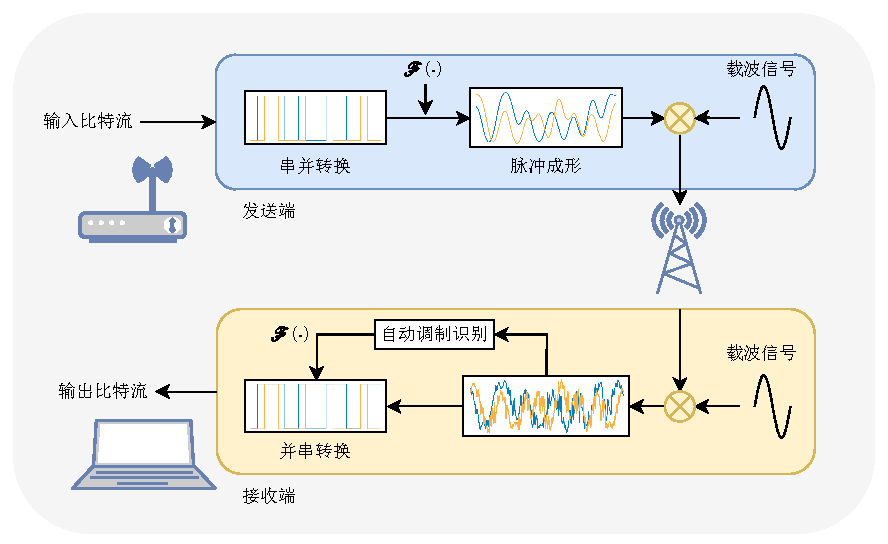
\includegraphics[width=\textwidth]{Image/AMC.pdf}
    \caption{自动调制识别在调制解调过程中的定位}
    \label{fig:AMR}
\end{figure}

随着无线通信技术的快速发展,尤其是在5G和即将到来的6G时代,通信技术正面临着更宽频段的拓展,以获取更多可用的频谱资源\cite{jdid2021machine}。这种需求促进了宽带信号采集技术的进步,特别是对宽频带电磁信号的瞬时采样。这种技术通过捕获宽频带电磁信号的瞬时状态,显著提高了空间电磁信号的捕获概率。然而,要保证信号的完整性,采样频率必须大于信号最高频率的两倍,这根据奈奎斯特采样定理而定。因此,满足宽带电磁频谱感知需求的同时,也带来了更高的硬件代价,如更大的采样速率和更高分辨率的模数转换器,同时也增加了数据处理的复杂性。

在这一背景下,如何在有限的能量和通信资源条件下,有效采集和处理宽带电磁频谱数据,成为了当前通信领域面临的一个重要挑战。自动调制识别作为解决这一挑战的关键技术之一,需同时应对信号的频道检测和调制方式识别,尤其在宽带信号的环境下面临更为复杂的挑战。因此,研究如何提高自动调制识别在宽带通信环境下的性能显得尤为重要。

\subsection{研究意义}\label{sec:background}

在当前的通信技术研究中,自动调制识别技术的重要性日益凸显。传统的自动调制识别算法,尽管在特定情况下有效,却常常受限于低识别准确率和高复杂度。这些局限性源于这些算法对信噪比的高依赖性,以及在处理高维数据时的计算负担。近年来,随着深度学习技术的快速发展和广泛应用,其在自动调制识别领域的应用展示出显著的优势,特别是在提高识别准确性和处理复杂信号方面。

然而,尽管深度学习方法在自动调制识别中取得了显著成果,但仍存在一些挑战和限制。首先,深度学习模型在低信噪比环境下的性能仍然受限。这一问题的根源在于深度学习模型通常需要大量的高质量数据来训练,而在实际应用中,尤其是在复杂或干扰环境中,高质量数据的获取可能非常困难。此外,深度学习模型的复杂性往往较高,这不仅增加了计算资源的需求,也限制了其在资源受限环境中的应用。

目前,自动调制识别领域的研究主要集中在窄带信号的识别上,即仅仅识别信号的调制模式。虽然这在一定程度上提高了通信系统的效率和可靠性,但对于现代通信系统而言,这远远不够。随着5G和预期中的6G技术的发展,宽带通信变得越来越普遍,对宽带信号的处理需求日益增长。在宽带信号的处理中,不仅需要识别信号的调制模式,还需要确定信号占用的子带位置。因此,基于宽带信号的自动调制识别,能够同时识别信号占用的子带位置及其对应的调制模式,成为了一个迫切需要解决的问题。

此外,从更具体的任务角度来看,基于深度学习的宽带调制信号的解调也需要一个更为完善的框架。这不仅涉及到识别子带位置和调制模式,还包括确定符号长度以确认最终调制结果的长度,最终输出宽带调制信号解调后的比特流。这一任务对于提高通信系统的数据传输效率和可靠性至关重要,尤其是在数据量巨大的宽带通信系统中。

结合目前学术界的研究进展,可以看到,虽然深度学习技术已经在自动调制识别领域取得了显著成果,但是在宽带信号处理和解调方面的研究仍处于起步阶段。未来的研究需要关注深度学习模型在低信噪比环境下的性能提升,以及如何减少对大量训练数据的依赖,同时降低模型的复杂度。此外,研究应当更加关注于宽带信号的处理,特别是在确定信号占用的子带位置及其调制模式方面的研究。这不仅将推动自动调制识别技术的发展,也将为未来的宽带通信技术提供重要的技术支撑,从而在更广泛的应用领域中发挥作用。

综上所述,深度学习在自动调制识别领域的应用前景广阔,但仍面临诸多挑战。随着通信技术的不断进步和深度学习技术的持续发展,我们有理由相信这些挑战将被逐步克服,深度学习将在自动调制识别领域发挥更加关键的作用。

% 随着无线通信技术的迅速发展,无线通信设备数量呈指数级增长。据统计预测,未来十年内,无线通信设备数量将增长1000倍。这些设备需时刻传输大量数据,使得频谱资源稀缺的状况更为紧迫。未来的网络中,无线通信系统需要在容量、频谱使用率和能耗效率方面实现10到1000倍的提升。为满足信息时代的万物互联及频谱资源高效利用等应用需求,电磁频谱感知成为信息时代可持续发展的关键。

% 当前,复杂的无线电磁环境对无线通信带来巨大挑战,信号在传输中容易扭曲和畸变,不利于解调。为提高频带利用率和通信速率,出现多种数字调制方式。这增加了接收端解调的难度,尤其在半协同或非协同通信中,接收端需在不知道先验信息的情况下判断调制方式。信号自动调制识别(Automatic Modulation Recognition, AMR)技术研究缓解了这一问题,为信号解调与处理奠定基础,对民用和军用领域都具有高研究价值。

% 信号自动调制识别技术的研究极大缓解了上述问题,自动调制识别介于信号检测与信号解调之间,为后续信号的解调与处理奠定基础。无论在民用还是军用领域都具有很高的研究价值。在民用方面,调制识别可以用于频谱检测和管理,以及识别干扰信号等。在军用领域常用于电子对抗,信息战中需要在截取无线电信息后快速检测其调制方式才能对信息进一步进行解密,也可用于对敌方通信进行干扰以掌握战争对主动权。此外,在主流通信技术中如果能够减少调制方式等先验信息的发送,不仅可以减少额外的频谱资源占用,还可以提高解码效率,降低通信时延。

% 现代5G和6G通信迎来更高更宽的频段拓展,以获取更多可用频谱资源。宽带信号采集技术通过对宽频带电磁信号的瞬时采样抓取,有效提高了空间电磁信号的捕获概率。然而,为保证信号完整性,根据奈奎斯特采样定理,采样频率必须大于信号最高频率的两倍。在满足空间宽带电磁频谱感知需求的同时,采样过程中需投入更高的硬件代价,如更大采样速率和更高分辨率的模数转换器,同时带来更复杂的数据处理。在有限的能量和通信资源下,有效采集宽带电磁频谱数据并在有限资源下实现高效信息压缩与传输,解决大范围下宽带信号的检测识别,是当前亟需解决的基础难题之一。宽带上的自动调制识别面临更为复杂的挑战,需要同时检测信号占用的信道和信号的调制方式。

% 近年来,随着计算机硬件水平的提升,深度学习技术成为焦点。作为机器学习的分支,深度学习以其层次结构和从浅层提取高阶特征的能力在多个领域取得成功。专家开始将深度学习引入通信领域,并发现其在自动调制识别方面表现卓越。

% \dots

% 自动调制识别是复杂电磁环境下信号感知和识别领域中的重要技术。传统的电磁认知识别方法依赖信号采集系统,但由于奈奎斯特采样定理,大数据量采集、传输、存储和处理成为挑战。压缩感知通过使用较小数据量的压缩信号取代奈奎斯特采样信号,极大缓解了信号处理中的瓶颈问题。深度神经网络通过从海量数据中自动提取信号特征,并进行后续识别,为复杂多变的电磁环境中的信号识别问题提供了新的解决方案。因此,基于压缩感知的智能宽带调制识别技术将成为未来研究的关键领域,涵盖宽带信号的压缩采样和调制识别两个方面。

\section{国内外研究现状}
技术领域内,特别是在通讯技术方面,信号调制识别的概念自20世纪初期就开始萌芽。这一时期,通信技术的专家们逐渐认识到,要想解读和理解目标信号中蕴含的关键信息,掌握其调制方式便成了一个不可或缺的步骤。因此,他们开启了针对信号调制方式识别的探索之旅。在最初阶段,这一工作主要依赖于从业人员根据个人经验进行手动识别。这个过程通常包括先对接收到的信号进行降频处理,以将高频信号转化为低频,随后依据信号波形的特定特征或特征组合来推断其调制方式。这种依靠个人判断的方法不仅容易出错,而且极度依赖于从业者的专业经验积累,尤其是在信号的信噪比较低的情况下,通过肉眼观察进行识别显得尤为困难。

随着移动通信技术的发展和现代战争模式的变化,信号调制识别的重要性日益凸显,促使更多的专业人士投入到这一领域的研究中,从而加速了相关技术的进步。特别是在20世纪60年代末期,斯坦福大学的Weaver与其研究团队发表的关键技术文档,代表了自动调制识别领域的一个重要进展。在该文档中,首次对外揭示了采用模式识别方法来快速自动辨认高频无线电信号调制方式的可能性,这一成果为自动调制分类技术带来了划时代的发展\cite{weaver1969automatic}。通过对信号频谱的数字化分析及利用最近邻模式识别器进行分类,实现了高精度的调制方式识别,这一研究成果奠定了自动调制识别研究的基础。

% 自那以后,自动调制识别技术的研究主要围绕两大核心方向展开:一方面是基于决策理论的最大似然假设检验方法;另一方面是采用基于特征提取的统计模式识别算法。此外,随着深度学习技术的快速发展,基于深度学习的调制识别算法也正受到广泛关注并处于积极研究阶段。这些技术的进步不仅极大提升了信号解调的速度和准确性,也为通信技术领域的发展开辟了新的道路。
\subsection{传统方法}
\subsubsection{似然比法}

基于决策理论的似然比假设检验方法,是植根于概率论领域的一种技术,它将调制方式的识别转换成了多重假设检验的问题。在这个过程中,接收到信号后立即对信号内的未知参数进行建模,以确定这些参数的概率分布特征。接下来,依据特定的似然准则,形成似然函数,并为各种可能的调制方式计算出相应的似然值。最后,通过应用贝叶斯信息准则(Bayesian Information Criterion, BIC)并设置适当的阈值,选择似然值最大的调制方式,作为对信号调制类型的预测。这一过程的关键步骤在图\ref{fig:likelihood}中以直观方式展示,以便更好地理解似然比假设检验在调制识别领域的实际应用。

\begin{figure}
    \centering
    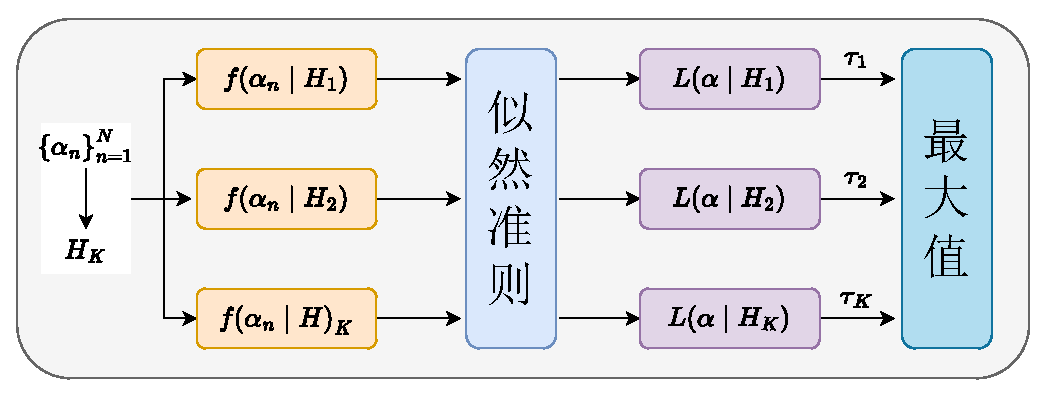
\includegraphics[width=\textwidth]{Image/likelihood.pdf}
    \caption{基于似然比检验的调制识别过程}
    \label{fig:likelihood}
\end{figure}

在基于似然比检验的调制识别方法的早期尝试中,尽管研究者们努力寻找最佳的分类规则,但长时间内成效有限。然而,在1988年,Kim和Polydoros的工作带来了一次飞跃,他们提出了一种名为平均似然比检验(Average Likelihood Ratio Test, ALRT)的算法\cite{kim1988digital}。此算法在高斯信道条件下,以调制信号的相位信息为基础,通过平均化处理构建似然函数,对BPSK和QPSK信号展现出优异的分类性能。1995年,Huang和Polydoros在ALRT算法的基础上进行了优化\cite{huan1995likelihood},提出了一种新型的准对数似然比(Quasi Log Likelihood Ratio, QLLR)分类器,不仅提高了MPSK信号的识别准确率,还扩展了算法的应用范围,覆盖了所有二维信号类型。通过对MQAM信号的研究,Yang等人\cite{yang1998log}证明了在信噪比高于12dB的条件下,ALRT算法能够实现100\%的识别率。进一步地,文献\cite{sills1999maximum}通过利用最大似然算法,成功实现了MPSK和MQAM信号的联合分类,并探究了在相干与非相干条件下分类性能的差异。

1998年,Boiteau等人引入了一种新的算法框架,即广义似然比检验(Generalized Likelihood Ratio Test, GLRT)\cite{boiteau1998general}。与ALRT算法相比,GLRT算法处理信号参数作为确定性未知变量,无需对信号或信道参数进行任何假设,减少了算法对信号先验知识的依赖,从而适用于更广泛的环境,并简化了算法复杂度。2000年,Panagiotou和Anastasopoulos在ALRT和GLRT的基础上,提出了混合似然比检验(Hierarchical Likelihood Ratio Test, HLRT)算法\cite{panagiotou2000likelihood},该算法能够根据多个未知参数进行建模,并根据不同参数采用不同的判决标准来构建似然函数,显示出对非恒包络调制信号有更高的识别性能。

近年来,决策理论下的调制识别算法研究持续深入。2013年,靳晓燕等研究人员提出一种新颖的通过查表方式简化最大似然算法的计算过程\cite{靳晓艳2013一种最大似然调制识别的快速算法},显著降低计算复杂度,使之适用于接收机进行实时信号处理。2015年,一项基于压缩感知框架的最大似然调制识别算法被提出\cite{童年2015非重构压缩样值的},能够在较少的数据量下实现更精确的识别结果。2016年,吴斌等人\cite{吴斌2016基于记忆因子的连续相位调制信号最大似然调制识别}利用最大似然算法构建记忆因子,应用于连续相位调制信号的识别中。最新的研究进展中,一种适用于多输入多输出(Multiple Input Multiple Output, MIMO)通信系统的最大似然识别算法被开发,该算法基于ALRT准则,构建了独立于天线数目和信道状况的似然函数,展现了增加天线数目有助于提升识别精度。在未知载波频率和符号速率的情况下,文献\cite{zhu2018likelihood}成功实现了MPSK和MQAM信号的有效分类。此外,一种在平坦衰落信道中有效工作的最大似然估计器也在文献\cite{chen2019faster}中提出。

\subsubsection{特征提取法}

基于特征提取的统计模式识别算法由于其强大的实用价值和相对简单的工程部署能力而受到广泛关注。这种方法的应用主要遵循三个核心步骤:信号预处理、特征提取、以及最终的分类器识别,其中特征提取阶段是整个过程中的关键。在信号预处理阶段,通过对信号执行一系列简单变换,例如滤波和降频处理,使信号规范化,降低了后续数据处理的复杂性。这个过程还包括清洗和筛选信号数据,以确保去除那些可能干扰识别准确性的非理想数据元素。图\ref{fig:feature_based}展示了基于特征提取的调制识别过程的主要步骤。

\begin{figure}
    \centering
    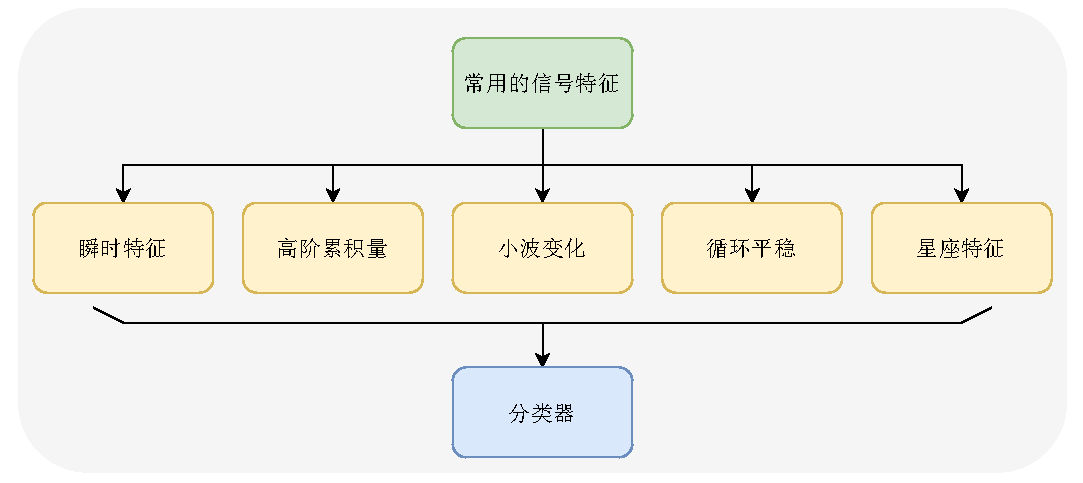
\includegraphics[width=\textwidth]{Image/feature.pdf}
    \caption{基于特征提取的调制识别过程}
    \label{fig:feature_based}
\end{figure}

特征提取阶段致力于在多个维度中发掘出不同调制方式之间的显著差异,由于不同特征可能反映出同一调制方式的不同调制信息,因此特征选择对于优化识别结果具有决定性影响。进而,在分类器识别阶段,通过利用精心挑选的特征,分类器能够有效区分不同的调制信号,这对于通信系统的效率和可靠性至关重要。

\subsubsection{瞬时特征法}
瞬时特征作为信号分析领域中的一种常用特征表示方法,因其获取便利性而广泛应用于信号调制识别。这些特征主要涵盖信号的幅度、相位和频率等方面。Nandi等人\cite{nandi1995automatic}开发出了多种基于瞬时特征的新方法,以实现对各种模拟信号的有效分类,并且在特定信噪比下达到了高达90\%的识别成功率。此外,在文献\cite{陈怀新2004基于统计特征主分量的信号调制识别}中主成分分析法等技术被用来对瞬时特征进行压缩,减少特征的维度,从而提升了调制识别的效率和精度。
\subsubsection{高阶累积量法}

高阶累积量作为一种反映信号统计特性的重要方法,特别是在抵抗高斯有色噪声方面显示出其独特的优势。信号的高阶统计特征被作为一种创新的特征参数用于信号调制识别,这一方法在低信噪比条件下也能实现可靠的识别性能。

\subsubsection{小波变换法}
小波变换技术因其在处理非平稳信号方面的有效性而在调制识别中占据了一席之地。通过小波变换得到的信号特征,尤其是那些能够揭示信号时频信息的特征,被文献\cite{刘明骞2018认知无线电}证明能够成功识别出不同的信号调制类型。此外,文献\cite{li2019wavelet}使用小波变换结合主成分分析和神经网络等先进技术在数字信号识别的准确度方面取得了显著提升。

\subsubsection{循环平稳特征法}
循环平稳特征利用信号的循环谱特性来区分不同的调制方式,有效地抑制了高斯噪声并揭示了调制相关的相位和频率信息。这些特征在处理多径信道条件下的信号识别问题时显示出了良好的性能。

\subsubsection{星座图特征}
星座图特征通过分析信号的星座图来直观地展现不同调制类型之间的差异,为调制识别提供了一个有效的途径。通过从星座图中提取的特定特征,结合先进的算法和技术,能够在不同信噪比条件下准确区分不同的调制信号。

\subsubsection{分类器选择}
最后,在选择合适的分类器方面,不同的机器学习算法可以根据其特点和应用场景的需求来优化调制识别过程。支持向量机、决策树、随机森林、最近邻分类器以及神经网络等,都是在不同数据规模和分类任务中常见的选择。神经网络特别适用于大规模数据训练,通过复杂的网络结构和大量的参数调整,可以建立复杂数据和分类结果之间的深层次联系,从而在分类任务中取得优异的表现。

\subsection{深度学习方法}
深度学习技术的快速发展为通信领域带来了创新的研究方向和解决方案,尤其在信号调制识别任务中表现出巨大的潜力和优势。不同于传统调制识别方法那样依赖于手工特征提取,深度学习算法通过其深层网络结构自动探索和学习数据中的复杂特征,无需人工干预即可挖掘出信号的本质特性。得益于大数据时代的到来,深度学习算法能够处理大量数据,通过这些数据训练出性能优异的识别模型。随着多个调制识别相关开源数据集的公开\cite{o2016convolutional}\cite{o2018over}及自动调制识别技术在军事及民用通信领域的广泛部署,近年来,深度学习驱动的自动调制识别技术受到了广泛关注。本节将对近年来深度学习在自动调制识别领域的研究进展进行综述。

卷积神经网络(Convolution Neural Network, CNN)模型展现了在处理具备空间属性数据(如图像分割、目标检测及分类)方面的显著优势。自动调制识别研究亦纳入CNN,借助其卓越的空间特征提取能力识别信号调制类型。根据输入数据的不同,基于CNN的自动调制识别模型分为两大类:一类是直接以原始I/Q数据为输入的CNN模型,另一类则处理经过预先处理的输入。除此此外,还有针对高效CNN架构的研究,旨在满足现代通信系统对延迟和复杂性的严格要求。

使用原始I/Q信号作为输入数据的CNN模型:2016年,采用简易四层CNN模型处理I/Q数据的方法初次被探讨,显示出超越多数传统方法的识别准确性\cite{o2016convolutional}。随后,Tekbıyık等人通过调整层数或超参数,提出了改进版CNN模型\cite{tekbiyik2020robust}。鉴于简单CNN架构可能未能充分提取I/Q信号中的代表性特征,进一步采用了复杂层次结构或变换操作的改进CNN模型,Liu等人受ImageNet 2015赛事获奖架构启发,提出基于残差网络(ResNet)和密集连接网络(DenseNet)的新型DL-AMR模型,以有效传递多层次学习特征至分类模块\cite{liu2017deep}。Zhang等人开发了一种实时信号调制分类模型,采用三级跳转残差网络识别调制信号,尽管识别准确性有所提高,但计算复杂性亦显著增加\cite{zhang2021real}。由于许多神经网络基模型直接借鉴于计算机视觉任务,这忽视了通信信号的固有属性。为解决此限制,Yashashwi等人提出在输入CNN模型前,估算接收信号的载波频率偏移和相位噪声,通过训练可调函数计算相位和频率偏移(校正参数),以减少偏移影响\cite{yashashwi2018learnable}。

使用预处理后的I/Q信号作为输入数据的CNN模型:由于原始信号经射频链路多环节处理及信道影响会丧失一些重要特性,如高阶累积量、频谱图和星座图等,直接使用原始I/Q信号作为输入的CNN模型的性能有限。而结合传统特征提取方法与CNN模型将有效地解决这一痛点,如Zeng等人通过短时离散傅立叶变换将一维无线电信号转化为频谱图像,进而通过高斯滤波降低噪声,提出的谱卷积网络模型实现了优于基准模型的识别准确率\cite{zeng2019spectrum}。Li等人提出的双谱-AlexNet方法将双谱的幅值谱输入CNN,有效抑制白噪声影响\cite{li2019automatic}。为提高非高斯噪声下识别性能,Ma等人引入循环相关熵谱,采用ResNet进行分类\cite{ma2019automatic}。此外,星座图作为AMR中另一广泛使用信号表示方法,可以从中直接提取特征确定调制方案。Peng等人将星座图转为3通道图像\cite{peng2018modulation},利用CNN模型处理彩色图像的能力进行分类。需要注意的是,正交幅度调制(QAM)模式间的混淆问题十分严重,为解决此问题,Wang等人采用两个CNN模型提升识别准确率,并分别以I/Q数据和星座图为训练数据\cite{wang2019data}。其中,基于星座图的CNN主要用于区分16QAM与64QAM的混淆问题。为充分利用循环谱图像的抗噪性和星座图提供的高阶调制识别能力,Wu等人设计了双分支CNN,提取多种特征后进行融合分类\cite{wu2019convolutional}。采用特征融合理念,Zhang等人实施了一种多模态融合模型,该模型结合了神经网络提取的不同图像特征与8个手工提取特征,以获得更区分度高的特征\cite{zhang2019automatic}。其他如眼图\cite{wang2017modulation}、特征点图像\cite{lee2019feature}及方形特征矩阵\cite{chen2021signet}等不同的输入信号表示形式也被尝试应用于自动调制识别模型中。

高效CNN架构设计:为满足超五代通信系统的预期延迟要求,Hermawan等人通过在每层中使用较少滤波器且减少可训练参数总数,开发了改进的基于CNN的自动调制识别模型\cite{hermawan2020cnn}。该模型处理时间低于0.01ms,符合超五代通信要求,尽管可训练参数数量减少,但仍保持较高的识别准确率。为应对5G业务对超高可靠性和低延迟的需求,Huynh-The等人提出了一种高效CNN模型,该模型在每个卷积块中并行采用多种非对称卷积核,并在网络中采用残差连接\cite{huynh2020mcnet}。Shi等人通过采用挤压-激励(Squeeze-and-Excitation, SE)块引入通道注意机制,实现了另一种更轻量级的模型\cite{shi2022combining}。

循环神经网络(Recurrent Neural Network, RNN)模型:无线通信信号除携带空间相关特性外,通常还包含时间相关特征,RNN模型则能很好捕捉序列中的时间关系。近年来,基于RNN的模型结构在自动调制识别领域取得良好性能,如Hong等人提出的基于RNN的AMR方法,利用GRU实现了优于部分CNN模型的识别准确率\cite{hong2017automatic}。Rajendran等人将I/Q信号转换为幅值和相位后输入到长短期记忆(LSTM)网络,实现高识别准确率\cite{rajendran2018deep}。以上仅使用两层RNN的模型已展现出在自动调制识别任务中的优异性能,证明了RNN在提取通信信号时间特征方面的能力。Ke等人设计了一个LSTM去噪自编码器,采用紧凑的RNN架构获取信号调制方案,在低成本计算平台上易于实现,同时达到了先进水平\cite{ke2021real}。

除了CNN和RNN模型外,近年来,随着Transfomer在自然语言处理领域的成功应用,也有研究者尝试将其应用于自动调制识别任务中。\cite{hamidi2021mcformer}提出了一种新颖的,基于Transformer的自动调制识别,利用其自注意力机制来捕捉信号中的长距离依赖关系,并于卷积神经网络所提取的特征进行对比和研究。文献\cite{tonchev2022automatic}中,作者利用图卷积神经网络(Graph Convolutional Network, GCN)探讨了各种调制模式之间的时间频域特征。

\section{本文主要贡献与创新}\label{sec:background}

\subsection{本文研究内容}\label{sec:background}

本论文延伸并深化了自动调制识别领域的研究,特别是在基于深度学习的宽带信号调制识别和调制解调技术方面。研究的意义可以从以下三个方面进行阐述:

1. 基于深度学习的自动调制识别:本论文致力于进一步提高调制识别的准确率和降低计算复杂度。通过应用深度学习模型,本文旨在更有效处理复杂的信号特征,提升在复杂无线电环境中的调制识别性能。这对于高效的通信技术发展提供了重要的技术支持。

2. 基于深度学习的宽带信号调制识别:本论文专注于宽带信号中占用的子带位置及其对应的调制模式的识别。这一研究不仅拓宽了自动调制识别的应用范围,也对于解决宽带信号处理中的新挑战,如频谱感知和频谱分配优化,具有至关重要的意义。通过深度学习技术的应用,能够有效识别并处理宽带信号中的多种调制模式,从而提升通信系统的灵活性和效率。

3. 基于深度学习的宽带信号调制解调:本论文还研究了宽带信号的调制解调过程,包括识别子带位置、调制模式和符号长度,进而输出宽带调制信号解调后的比特流。这一部分的研究不仅提升了调制识别的准确性和效率,而且实现了从信号检测到信息恢复的完整流程,极大提升了宽带信号处理的实用性和灵活性。

总体来说,本论文在基于深度学习的自动调制识别技术的基础上,通过拓展到宽带信号的识别和解调,开辟了通信技术在更广阔领域内应用的新视角,为未来通信系统的发展提供了新的可能性和解决方案。

\subsection{本文研究创新点}\label{sec:background}

本研究致力于解决宽带信号处理中的几个关键问题,主要集中在信号调制识别、宽带信号的信道识别与调制识别、以及宽带信号的解调三个方面。研究内容包括自适应噪声矫正模块的开发,多陪集采样的应用,以及利用神经网络进行宽带信号解调的创新性工作。

1. 提升自动调制识别在低信噪比下的准确率

在信号调制识别方面,本研究引入了一种先进的自适应噪声矫正模块,旨在缓解噪声对信号识别准确性的负面影响。该模块采用动态调整机制,根据环境噪声水平的实时变化,自动调节矫正强度,从而提高信号调制识别的鲁棒性。这一模块的引入,显著提升了在多变和复杂噪声环境下的信号调制识别系统性能,提高了不同调制模式的区分能力。

2. 实现宽带信号调制识别与信道识别

针对宽带信号处理中的采样挑战,本研究采用了多陪集采样策略,目的是提升宽带信号的采样效率,并全面捕捉其频谱信息。此外,本研究采用了基于神经网络的方法,实现了对宽带信号的信道识别与调制识别的高效处理。所提出的神经网络模型能够同时处理信号的信道占用和调制模式识别任务,为宽带信号的高效分析提供了一种新的途径。

3. 为宽带信号解调提供一个完整的框架

在宽带信号的解调阶段,本研究提出了一套综合性解决方案。在完成信道与调制识别的基础上,研究重点转向如何有效提取信号对应的比特流。经过深入的研究和创新设计,我们开发了一种有效的宽带信号解调算法,使系统能够准确而高效地重构原始信号的信息,满足现实世界应用中对数据准确性和传输效率的严格要求。

总体而言,本文通过研发自适应噪声矫正模块、应用多陪集采样技术对宽带信号进行采样和利用神经网络进行信号识别解调,全面探索了宽带信号处理的关键问题,并在信号调制识别、信道与调制识别、以及宽带信号解调等多个方面取得了较好成果。未来,我们计划深化这些研究,进一步优化这些技术,以适应日益发展的通信技术和不断变化的通信环境。同时,我们鼓励对这些技术在实际应用场景中进行更广泛的验证和探索,以确保它们在真实环境中的有效性和可靠性。

\section{论文结构}\label{sec:background}
本论文共分为五章,各章节内容安排如下:

本论文深入研究了自动调制识别与解调技术,在六个章节中系统地阐述了相关理论、实践方法及其创新点。以下为每个章节的简介:

第一章:绪论

本章介绍了研究的背景和意义,着重指出了自动调制识别技术在现代通信系统中的重要性。论文概述了自动调制识别与解调技术的研究现状,包括传统方法和近年来兴起的深度学习方法。此外,本章还阐明了本文的主要研究内容和结构安排,为读者提供了研究的总体框架和研究方向。

第二章:调制识别的理论基础

本章详细介绍了调制识别的理论基础,包括基本的调制原理、信号模型及其特性。本章还讨论了传统的调制识别技术,如特征提取法和似然比法,以及这些技术的局限性。此章节为理解后续章节中提出的方法奠定了坚实的理论基础。

第三章:窄带信号调制识别

本章中,提出了一种创新的自适应噪声矫正的针对窄带信号的调制识别网络。该章节详细介绍了网络的设计思想、结构以及工作原理。此外,还阐述了如何通过自适应调整来优化噪声矫正效果,从而在复杂噪声环境下提高调制识别的准确性和鲁棒性。

第四章:宽带信号调制识别与信道识别及解调

本章专注于宽带信号的处理,特别是调制识别与信道识别的问题。本章探讨了宽带信号特有的挑战,如高采样率和数据处理的复杂性,并介绍了采用多陪集采样等技术应对这些挑战的方法。深入研究了宽带信号的识别与解调过程。本章详细描述了如何从宽带信号中提取有效信息并进行准确的解调,以得到原始信号的比特流。此外,本章还讨论了神经网络在宽带信号解调中的应用及其优势。

第五章:总结与展望

在最后一章中,本文总结了整个研究的主要成果和贡献。同时,对研究中存在的局限性和未来可能的研究方向进行了讨论。本章为整个研究提供了一个全面的回顾,并对未来自动调制识别技术的发展趋势提出了展望。

\begin{figure}[htbp]
    \centering
    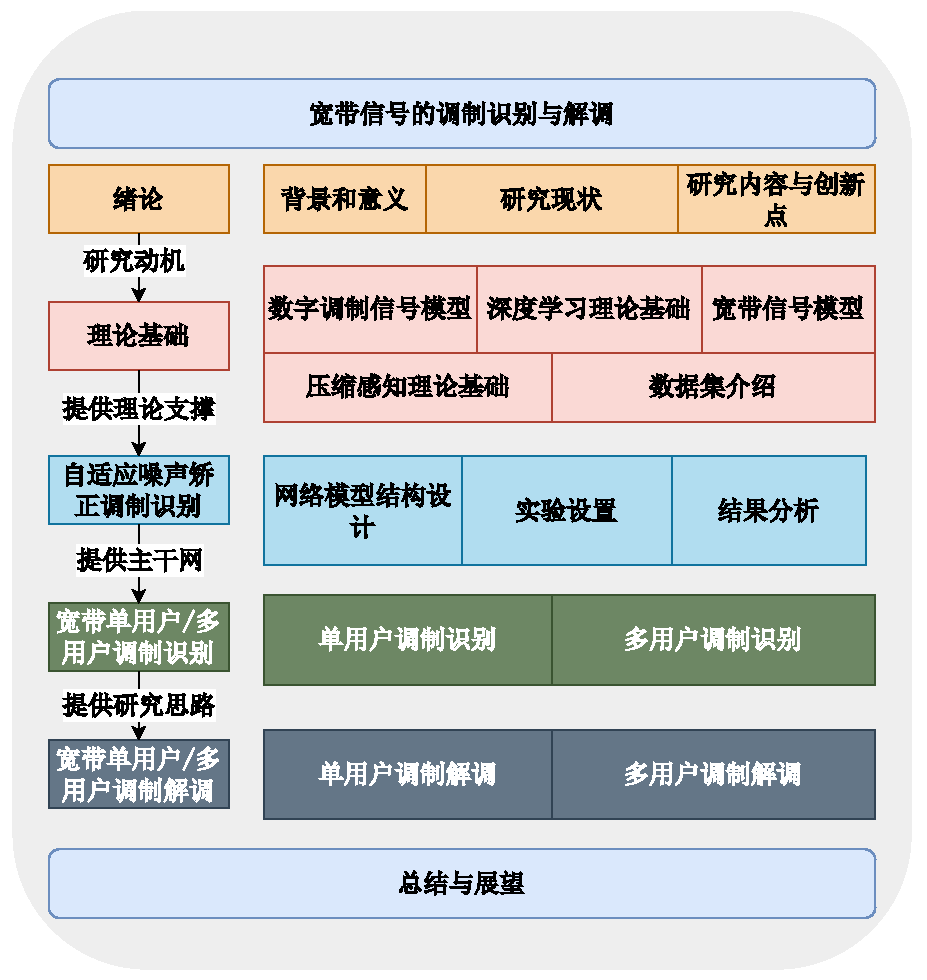
\includegraphics[width=\textwidth]{Image/chap1_overallstructure.pdf}
    \caption{论文结构}
    \label{fig:thesis_structure}
\end{figure}

\chapter{调制识别的理论基础}\label{chap:intro}
\markboth{第二章\ \ 调制识别的理论基础}{}
% ### 章节大纲

% 1. **引言**
%    - 研究背景与目的
%    - 章节内容概述

% 2. **数字调制信号模型**
%    - 数字调制的基本原理
%    - 常见数字调制类型及其数学模型
%    - 调制信号的图形表示

% 3. **传统调制识别方法分析**
%    - 传统方法概述
%    - 各种传统方法的优势与局限性
%    - 传统方法的历史贡献

% 4. **深度学习在调制识别中的应用**
%    - 深度学习方法概述
%    - 特征提取能力与应用优势
%    - 深度学习方法的实际应用案例

% 5. **宽带信号处理的挑战与解决方案**
%    - 宽带信号处理的问题阐述
%    - 多陪集采样原理及应用
%    - 压缩感知理论在调制识别中的应用

% 6. **数据集介绍与评估方法**
%    - 常用数据集的介绍
%    - 数据集在调制识别评估中的作用
%    - 实验设计与性能评估标准

% 7. **总结**
%    - 本章重点回顾
%    - 对后续研究章节的铺垫

% 通过本章的详细介绍,读者将能够全面理解调制识别领域的理论基础,为深入了解后续的具体研究方法和实验设置打下坚实的基础。



\section{引言}\label{sec:background}
% 本章旨在为调制识别领域的理论基础提供全面的介绍。首先,我们将对数字调制信号模型进行详细阐述,通过数学公式和图像两个角度对常见的数字调制模式进行全面描述,为后续调制识别任务建立主观认知基础。传统调制识别方法是研究的重要组成部分,本章将从多个角度对传统方法进行分析,深入挖掘其优缺点,为后续工作提供深刻启发,突显传统方法在调制识别领域的历史贡献。通过对传统方法的全面了解,我们能更好地把握调制识别问题的本质,为提出更创新、更高效的解决方案奠定坚实基础。

% 随后,我们将重点介绍目前主流的深度学习方法在调制识别中的应用。深度学习在自动调制识别领域取得显著进展,其强大的特征提取能力为调制识别任务带来新的视角。通过深入学习深度学习理论,我们能更好地理解并应用这一跨学科领域的理论,为实际问题的解决提供新的思路。本课题的创新点之一是宽带调制信号的识别与解调,为了解决采样与存储的难题,我们引入了压缩感知理论,这部分将详细阐述多陪集采样的基本原理及其在宽带调制信号处理中的应用,为后续章节的具体方法和算法提供理论支持。最后,我们将介绍一些常用的数据集,这些数据集将为后续内容提供坚实的实验基础。通过对这些数据集的了解,我们能更全面地评估不同方法在真实场景中的性能,并为调制识别领域的实证研究提供可靠的数据支持。在理论基础的系统构建后,我们将深入探讨调制识别方法的设计与实现,为该领域的进一步研究奠定扎实基础。

本章旨在全面介绍调制识别领域的理论基础,既包括数字调制信号模型的深入阐述,也包括对传统调制识别方法和当前的深度学习方法的详尽分析。通过这一综合性的理论框架,本研究为后续工作建立了坚实的基础,特别是针对宽带调制信号的识别与解调所面临的挑战。

首先,本章将详细描述数字调制信号模型,通过精确的数学公式和直观的图像展示来全面描述常见的数字调制模式。这一部分的目的是为读者建立关于不同调制类型的清晰认识,为理解调制信号的复杂性和多样性提供必要的背景。
% 接着,本章将深入探讨传统调制识别方法。这些方法的历史和发展对于理解调制识别问题至关重要。我们将从多个角度分析这些方法,深入挖掘它们的优势和局限,从而为后续工作提供深刻的见解。此外,通过突出传统方法在调制识别领域的历史贡献,本章将展示这些技术是如何为现代方法铺平道路的。
在第一章中已经详细地介绍了传统调制识别方法的基础以及相应的弊端,本章将转向目前主流的深度学习方法在调制识别中的应用。深度学习的引入在自动调制识别领域引发了一场变革,特别是其在特征提取方面的强大能力。我们将探讨深度学习如何为解决复杂的调制识别问题提供新的思路和方法。为了解决宽带调制信号处理中的采样和存储挑战,本章将详细阐述多陪集采样的基本原理及其在宽带信号处理中的应用。通过引入压缩感知理论,本研究为高效处理宽带信号提供了理论支持。这一创新点是本研究的重要组成部分,将在后续章节中进一步发展。最后,本章将介绍一些常用的数据集,并解释这些数据集在评估不同调制识别方法中的作用。这些数据集不仅为实证研究提供了坚实的基础,也使我们能够全面评估各种方法在实际应用中的性能。

通过这些内容的系统介绍,本章为探讨调制识别方法的设计与实现奠定了坚实的理论基础,并为该领域的进一步研究提供了必要的背景和知识。

\begin{figure}
    \centering
    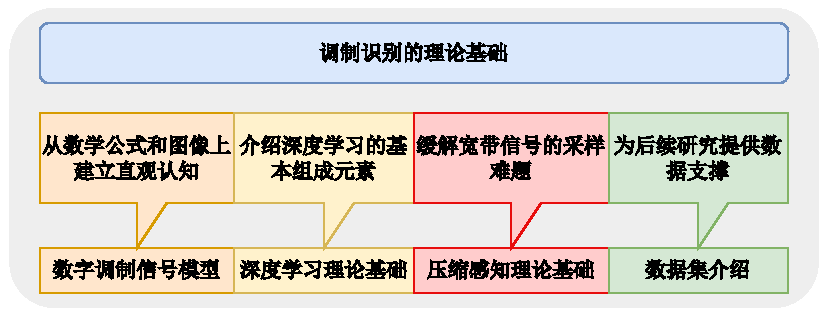
\includegraphics[width=\textwidth]{Image/chap2_map.pdf}
    \caption{本章大纲}
    \label{fig:outline2}
\end{figure}

\section{数字调制信号模型}\label{sec:background}
数字通信是现代通信技术中的一种核心模式,其主要原理在于将离散的数字信号源转换为用于传输的时间连续信号。相较于传统的模拟通信,数字通信系统展现出显著的优势,例如更高的信号传输质量和更强的干扰抵抗能力。特别是在可靠性方面,数字信号可以通过编码来增强,使其在复杂的通信环境下保持较高的传输稳定性。此外,数字信号的离散性质使得它们易于通过计算机进行处理,从而大幅提升了通信系统的效率和灵活性。

在数字通信系统中,调制技术起着至关重要的作用。它涉及到将数字数据转换为适合在物理媒介(如无线电波)上传输的信号的过程。主要的数字调制技术包括幅移键控(Amplitude Shift Keying, ASK)、频移键控(Frequency Shift Keying, FSK)、相移键控(Phase Shift Keying, PSK)和正交振幅调制(Quadrature Amplitude Modulation, QAM)。这些调制技术通过改变载波信号的不同特性(如幅度、频率或相位)来代表数字数据。

本节将深入探讨这些数字调制技术的原理和特点,为理解它们在调制识别中的应用提供坚实的理论基础。通过对这些调制技术的详细介绍,本文旨在建立对数字调制过程的全面理解,为后续探讨调制识别的先进技术和方法奠定基础。

\subsection{幅移键控}\label{sec:background}
% 在幅移键控中,数字信息被转换为不同的振幅水平。信号的振幅随着数字信号的变化而改变,从而产生调制后的信号,其数学表达式为:
% \begin{equation}
%     s_{MASK}(t) = A \sum_n a_n g_T (t-nT_s) \cos(2\pi f_c t),
% \end{equation}
% 公式中,$a_{n} \in \{\pm 1, \pm 3, \dots, \pm(M-1)\}$。

% 通常,ASK用于调制二进制信号,其中0和1分别对应于两个不同的振幅水平。 如果要发送数字1,则信号振幅增加到特定水平;如果要发送数字0,则信号振幅减小到另一个特定水平。接收端测量接收到的信号的振幅,并根据振幅的不同来判断发送的是0还是1。
% 图~\ref{fig:ASK}展示了ASK的示意图。

幅移键控(ASK)是一种基本的数字调制技术,它通过改变信号的振幅来传输数字信息。在ASK中,数字信号被转换成不同的振幅水平,从而实现数据的传输。这种调制技术的关键在于,它直接调节载波信号的幅度,以代表数字数据。ASK信号的数学表达式如下:

% ### 数学表达式
\begin{equation}
    s_{MASK}(t) = A \sum_n a_n g_T (t-nT_s) \cos(2\pi f_c t),
\end{equation}
其中,\( A \) 是载波的振幅,\( a_n \) 是表示数字信息的振幅系数,\( g_T(t) \) 是脉冲形状函数,\( T_s \) 是符号周期,\( f_c \) 是载波频率。\( a_n \) 的取值通常是 \(\{\pm 1, \pm 3, \dots, \pm(M-1)\}\),这里的 \( M \) 表示振幅的不同水平数量。

% ### 二进制ASK
在二进制ASK中,只使用两个振幅水平来表示数字0和1。例如,当需要传输数字1时,信号的振幅被设置为较高的水平;相反,传输数字0时,则将振幅设置为较低的水平。接收端通过测量接收信号的振幅并比较预定义的阈值,来确定传输的是0还是1。其主要有如下特点:

% ### ASK的特性与适用场景
简单性:ASK调制技术因其实现简单而被广泛应用,尤其适用于带宽受限和系统复杂度要求低的通信系统。

功耗:由于ASK直接调制振幅,因此在某些情况下可能比其他调制技术(如FSK或PSK)更耗电。

抗干扰能力:ASK对噪声较为敏感,特别是在信号强度低的情况下,噪声可能会导致错误的数据解读。

适用范围:ASK常用于短距离和低速率的通信,例如无线射频识别(RFID)和一些无线传感器网络。

% ### 总结
幅移键控作为一种基础的数字调制技术,在特定的应用场景下具有其独特的优势。尽管存在一些局限性,如对噪声的敏感性和较高的功耗,ASK仍然是数字通信中不可或缺的一部分。对ASK技术的深入理解,对于全面掌握数字调制的理论和实践具有重要意义。图~\ref{fig:ASK}所示为幅移键控的示意图,展示了4ASK中不同数字状态对应的振幅变化。通过这种直观的表示,可以清晰地理解ASK调制信号的基本原理和特点。

\begin{figure}[htbp]
    \centering
    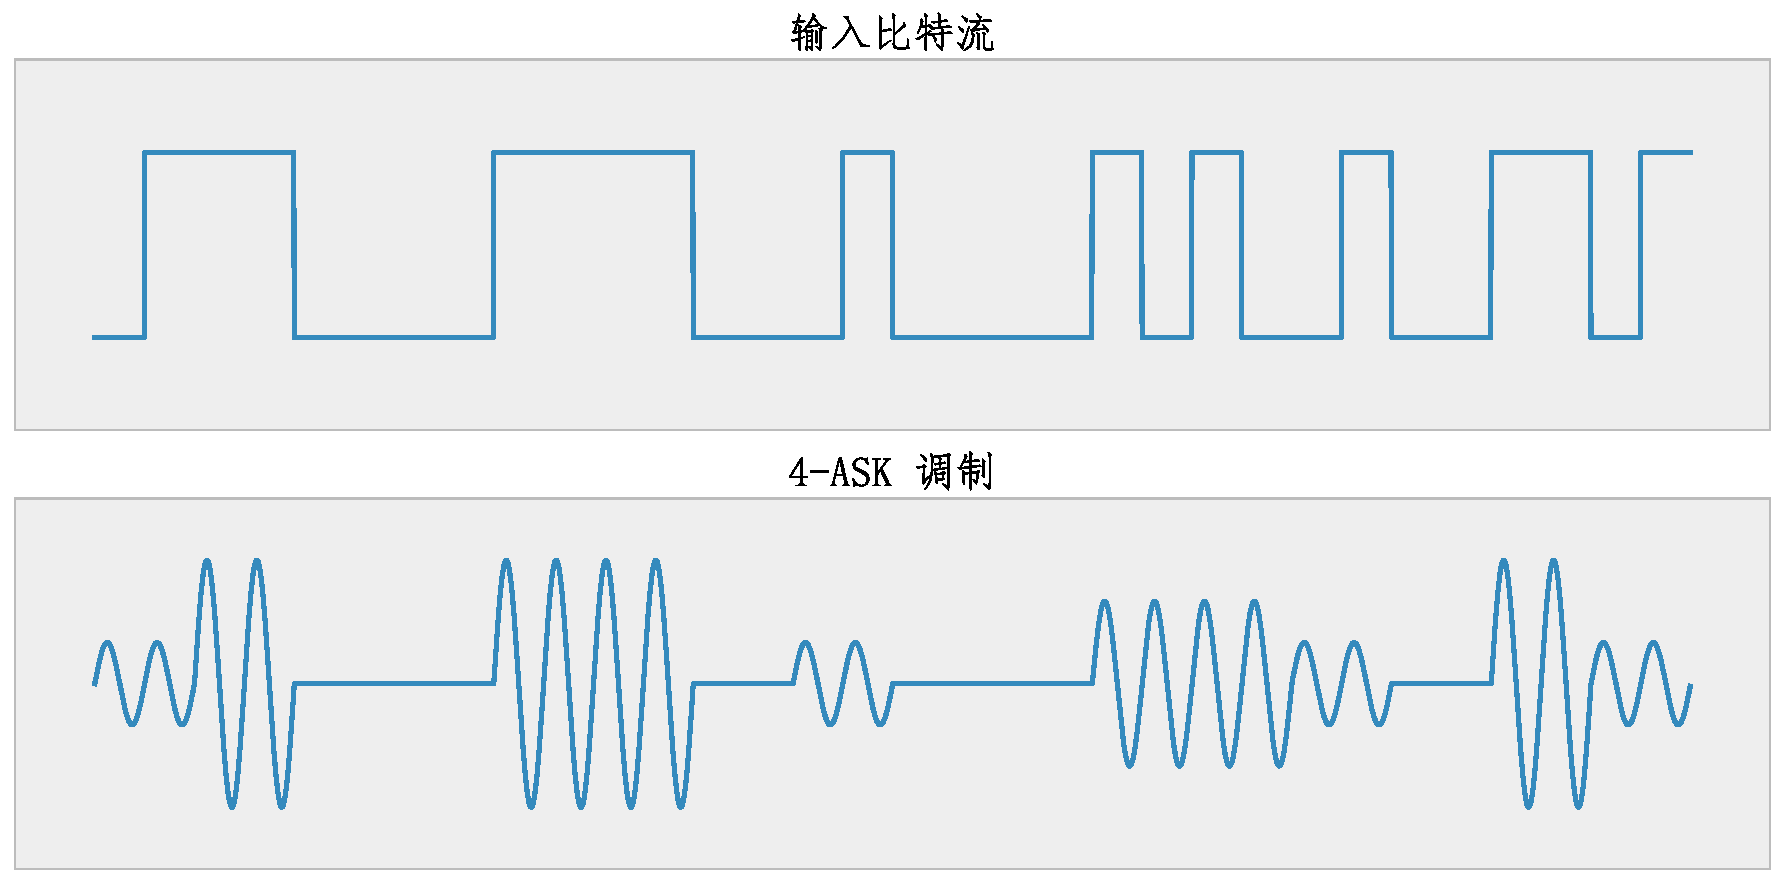
\includegraphics[width=\textwidth]{Image/ask.pdf}
    \caption{幅移键控示意图}
    \label{fig:ASK}
\end{figure}


\subsection{频移键控}\label{sec:background}
% 频移键控是一种将数字信息转换为频率变化的数字调制技术。通常,两个不同的频率代表二进制的0和1。
% \begin{equation}
%     s_{2FSK}(t) = \begin{cases}
%         A \cos(2\pi f_1 t), & a_n = 0 \\
%         A \cos(2\pi f_2 t), & a_n = 1
%     \end{cases}, (n - 1/2)T_b \leq t < nT_b \\
% \end{equation}
% 其中,$A$为信号幅度,$f_1$和$f_2$为信号频率,$T_b$为符号持续时间,$a_n$为比特值。

% 如果要发送数字1,则载波频率切换到一个特定频率;如果要发送数字0,则载波频率切换到另一个特定频率。接收端测量接收到的信号的频率,并根据频率的不同来判断发送的是0还是1。相对于ASK,FSK在噪声环境中表现更好,因为噪声对频率的影响相对较小。

% 多元频移键控(M-ary Frequency Shift Keying,MFSK)可以表示为:
% \begin{equation}
%     s_{MFSK}(t) = Ag(t) \cos(2\pi f_n t), (n - 1) T_s \leq t \leq nT_s
% \end{equation}
% 其中,
% \begin{equation}
%     f_n = f_c + \frac{(2i - M - 1)}{2} \Delta f, i = 0, 1, \dots, M - 1
% \end{equation}
% $f_c$为载波频率,$\Delta f$为频率间隔,$M$为调制阶数。图~\ref{fig:FSK}展示了FSK的示意图。

频移键控(FSK)是一种通过改变载波信号的频率来传输数字信息的调制技术。在FSK中,数字信息(如二进制的0和1)被转换为不同的频率变化。这种调制技术特别适用于需要在噪声环境下传输数据的通信系统,因为相对于幅度变化,频率变化对噪声更具抵抗力。二进制频移键控(2FSK)的数学表达式如下:

% ### 数学表达式
\begin{equation}
    s_{2FSK}(t) = \begin{cases}
        A \cos(2\pi f_1 t), & a_n = 0 \\
        A \cos(2\pi f_2 t), & a_n = 1
    \end{cases}, (n - 1/2)T_b \leq t < nT_b \\
\end{equation}
其中,\( A \) 表示信号幅度,\( f_1 \) 和 \( f_2 \) 分别代表两个不同的频率,\( T_b \) 为比特持续时间,\( a_n \) 为比特值。

在发送数字1时,载波频率切换到 \( f_2 \);相反,发送数字0时,载波频率切换到 \( f_1 \)。接收端通过测量接收信号的频率来确定发送的是0还是1。FSK的主要特点如下:

% ### FSK的特性与应用
抗干扰能力:FSK由于其频率变化特性,在噪声环境中的表现优于幅度变化调制(如ASK),因此在无线通信和数据传输中得到了广泛应用。

功耗:与ASK相比,FSK通常需要更高的带宽,但它提供了更好的信号稳定性和抗干扰能力。

% ### 多元频移键控(MFSK)
MFSK是FSK的一种扩展,它使用多个频率来表示更多的符号,从而提高数据传输速率。
\begin{equation}
    s_{MFSK}(t) = Ag(t) \cos(2\pi f_n t), (n - 1) T_s \leq t \leq nT_s
\end{equation}
其中,
\begin{equation}
    f_n = f_c + \frac{(2i - M - 1)}{2} \Delta f, i = 0, 1, \dots, M - 1
\end{equation}
\( f_c \) 为载波频率,\( \Delta f \) 为频率间隔,\( M \) 为调制阶数。MFSK允许系统在相同的带宽下传输更多的数据,但随着调制阶数的增加,系统的复杂度也会相应提高。

% ### 总结
频移键控因其在噪声环境中的优异表现,以及相对较高的信号稳定性,成为了数字通信中一种重要的调制技术。通过对FSK及其变体MFSK的深入理解,可以更好地把握数字调制过程的特性和应用场景。图~\ref{fig:FSK}所示为频移键控的示意图,展示了不同数字状态下载波频率的变化,直观地反映了FSK调制信号的基本原理和操作方式。

\begin{figure}[htbp]
    \centering
    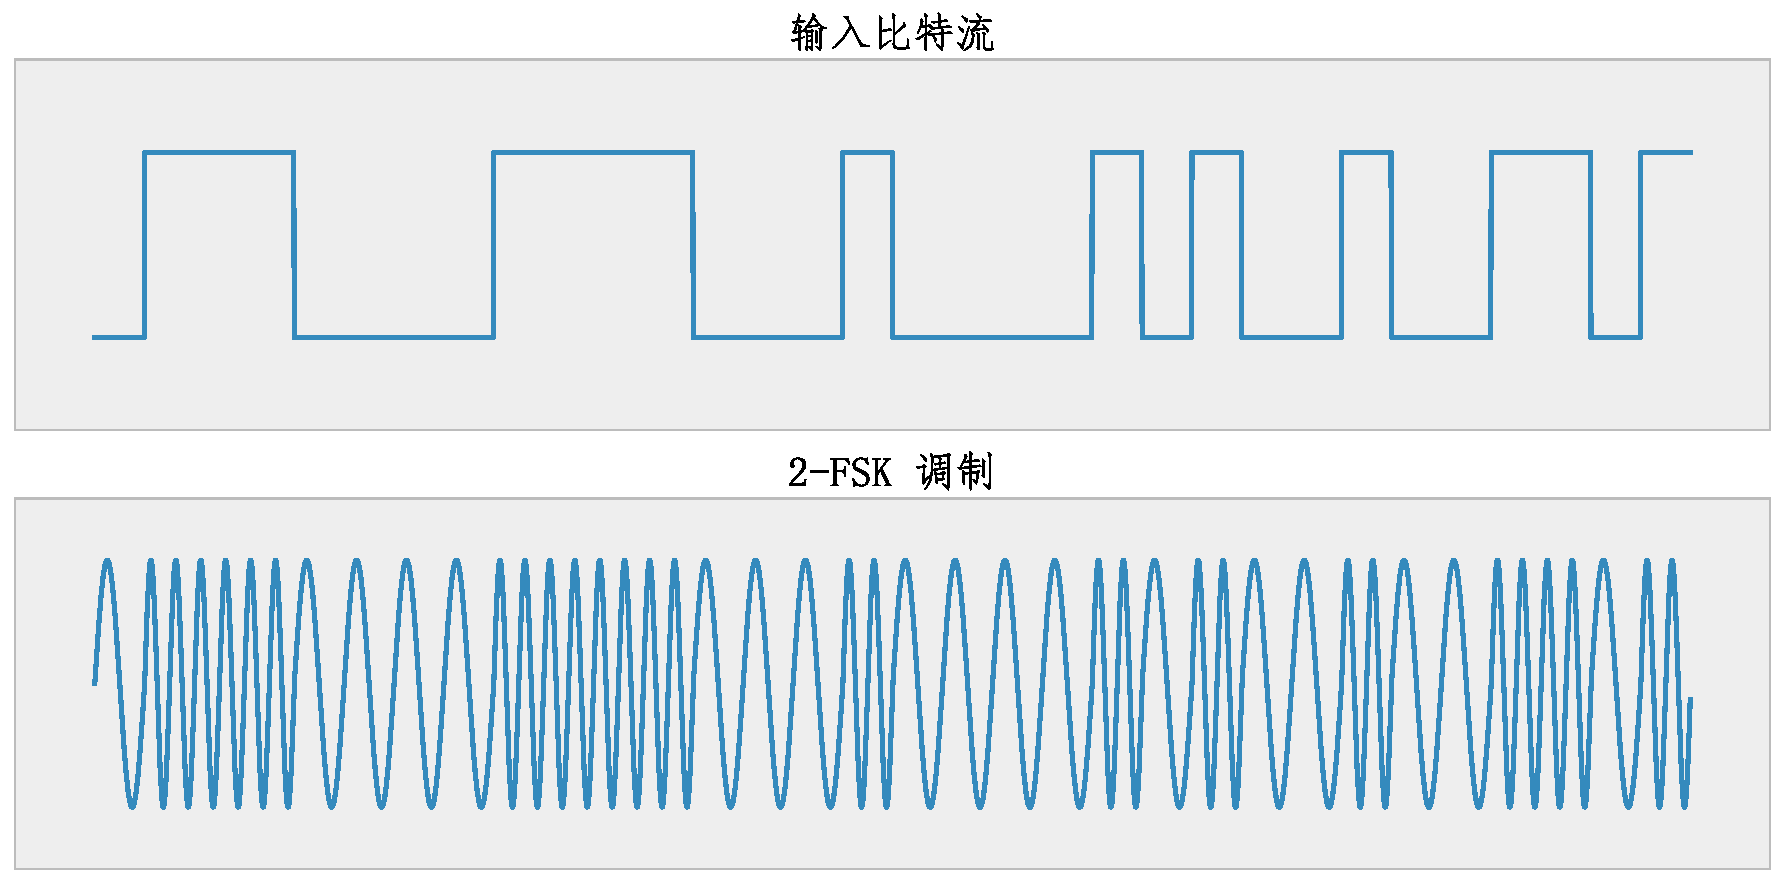
\includegraphics[width=\textwidth]{Image/fsk.pdf}
    \caption{频移键控示意图}
    \label{fig:FSK}
\end{figure}

\subsection{相移键控}\label{sec:background}
% 相移键控中数字信息通过改变载波信号的相位来传递。通常,两个或多个不同的相位表示不同的数字符号。
% \begin{equation}
%     s_{MPSK}(t) = g(t) \cos(2\pi f_c t + \frac{2\pi}{M} (m-1)),
% \end{equation}
% 其中,$g(t)$为基带脉冲成形滤波器,$\theta_m = \frac{2\pi}{M} (m-1)$表示第m个传输符号的载波相位。图~\ref{fig:PSK}展示了PSK的示意图。

% 如果要发送数字1,则载波的相位发生变化到一个特定的角度;如果要发送数字0,则载波的相位发生变化到另一个特定的角度。接收端测量接收到的信号的相位,并根据相位的不同来判断发送的是0还是1。 PSK的带宽效率通常比ASK更高,因为信息通过相位变化而不是振幅变化来传递。PSK在一定程度上对噪声具有抗性,但不如FSK那样抗噪声。PSK相对于ASK和FSK来说更复杂,因为它涉及到相位变化的处理。
相移键控(PSK)是一种将数字信息转换为载波信号相位变化的调制技术。PSK通过改变载波的相位来传输不同的数字符号,通常使用两个或多个不同的相位来表示不同的数字状态。PSK信号的数学表达式如下:

% ### 数学表达式
\begin{equation}
    s_{MPSK}(t) = g(t) \cos(2\pi f_c t + \frac{2\pi}{M} (m-1)),
\end{equation}
其中,\( g(t) \) 是基带脉冲成形滤波器,\( f_c \) 是载波频率,\( \theta_m = \frac{2\pi}{M} (m-1) \) 表示第 \( m \) 个传输符号的载波相位。在二进制PSK中,通常使用两个相位(如0和180度)来表示数字0和1。例如,如果要发送数字1,则载波的相位变化到特定的角度;相反,如果要发送数字0,则载波的相位变化到另一个特定的角度。接收端测量接收到的信号的相位,并根据相位的不同来判断发送的是0还是1。PSK的主要特点如下:

% ### PSK的特性与应用
带宽效率:相对于ASK,PSK具有更高的带宽效率,因为它通过相位变化而不是振幅变化来传递信息。

抗噪声能力:PSK在一定程度上对噪声具有抗性,尤其是在相位同步良好的条件下,但它的抗噪性不如FSK。

复杂性:相对于ASK和FSK,PSK的实现更为复杂,特别是在处理相位变化方面。

% ### 多元相移键控(MPSK)
MPSK是PSK的一种扩展,它使用多个相位来表示更多的符号,从而提高数据传输速率。每个符号通过一个特定的相位来表示,增加了调制的阶数,从而允许更多数据在相同的带宽内传输。

% ### 总结
PSK作为一种重要的数字调制技术,在数字通信中被广泛应用,特别是在需要高带宽效率和适度抗噪声能力的场景。尽管PSK相对于ASK和FSK更为复杂,但它在许多通信系统中因其带宽效率和性能优势而被广泛采用。图~\ref{fig:PSK}所示为相移键控的示意图,清晰展示了PSK调制信号的基本原理,包括如何通过载波的相位变化来表示不同的数字状态。通过对PSK的深入理解,可以更好地掌握数字调制技术的多样性和其在现代通信系统中的应用。

\begin{figure}[htbp]
    \centering
    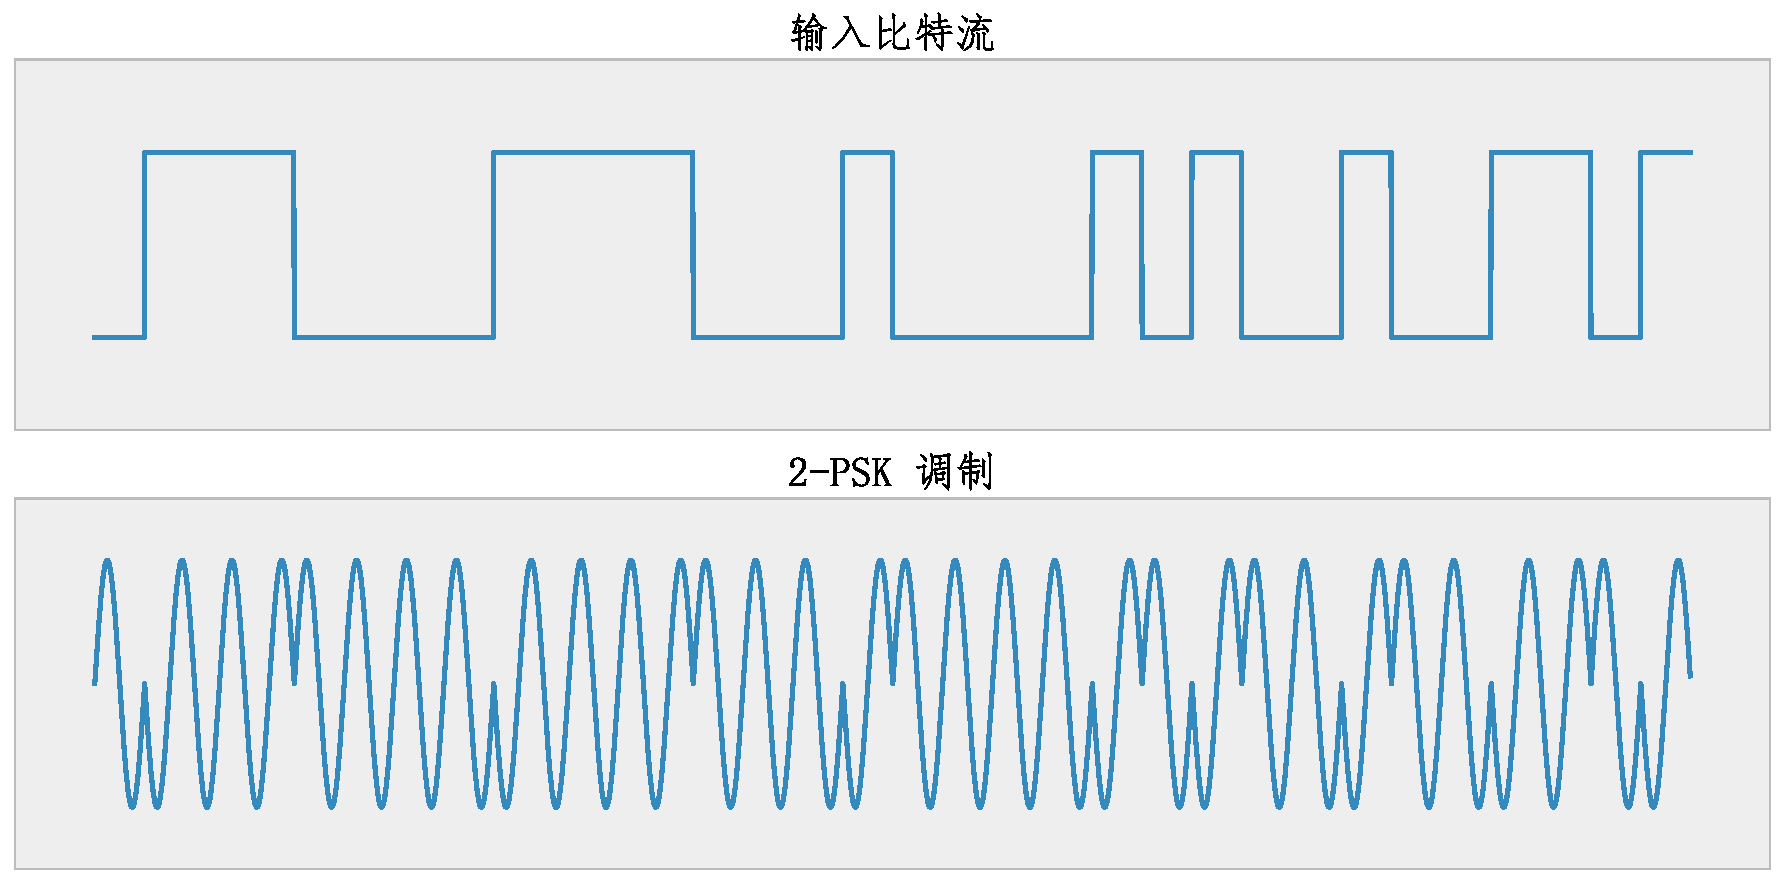
\includegraphics[width=\textwidth]{Image/psk.pdf}
    \caption{相移键控示意图}
    \label{fig:PSK}
\end{figure}


\subsection{正交振幅调制}\label{sec:background}
% 正交振幅调制在信号中同步调制了振幅和相位信息。通常,QAM信号可以表示为在信号空间中的点,其中两个正交的轴分别表示振幅和相位。
% \begin{equation}
%     S_{QAM}(t) = Aa_{cn}g_T(t)\cos(2\pi f_c t) - Aa_{sn}g_T(t)\sin(2\pi f_c t),
% \end{equation}
% 其中,$a_{cn}$和$a_{sn}$分别表示当前传输比特的星座点位置坐标,分别对应了同相支路和正交支路的比特符号。图~\ref{fig:QAM}展示了QAM的示意图。

% QAM通过同时改变振幅和相位来表示数字信息。例如,如果要发送数字11,则信号空间中的点将具有特定的振幅和相位。接收端测量接收到的信号的振幅和相位,并根据这些信息还原发送的数字信息。QAM可以在有限的频谱内传输多个位,因此具有很高的带宽效率。相较于ASK、FSK和PSK,QAM的调制和解调过程更为复杂。
正交振幅调制(QAM)是一种先进的数字调制技术,它通过同时调制信号的振幅和相位来传输数字信息。QAM的独特之处在于它利用信号空间的两个正交维度(即振幅和相位)来表示数据,使得每个符号可以携带更多的信息位。

% ### 数学表达式
QAM信号的数学表达式如下:
\begin{equation}
    S_{QAM}(t) = Aa_{cn}g_T(t)\cos(2\pi f_c t) - Aa_{sn}g_T(t)\sin(2\pi f_c t),
\end{equation}
其中,\( A \) 是载波的振幅,\( g_T(t) \) 是脉冲形状函数,\( f_c \) 是载波频率。\( a_{cn} \) 和 \( a_{sn} \) 分别表示当前传输比特在星座图上的坐标,对应于同相(Inphase)和正交(Quadrature)支路的比特符号。其主要特点如下:

% ### QAM的特性与应用
带宽效率:QAM能够在有限的频谱内传输大量数据,因此具有较高的带宽效率。这使得QAM在需要高数据速率的通信系统中特别有价值。

信号空间:QAM信号可以在信号空间中的点上表示,这些点在两个正交轴上分布,分别代表振幅和相位的不同组合。

复杂性:与ASK、FSK和PSK相比,QAM在调制和解调方面更为复杂。它需要精确的幅相平衡和同步,才能准确地检测信号空间中的点。
抗干扰能力:虽然QAM在抗噪声方面不如某些其他调制方式,但它通过适当的星座图设计和前向纠错编码等技术可以提高抗干扰能力。

% ### 总结
QAM因其高效的带宽利用率在现代通信系统中发挥着重要作用。它通过综合调制振幅和相位,能够在每个符号中携带更多的信息位。尽管QAM的实现相对复杂,但它在高速数据通信领域的应用优势使其成为数字调制技术中的重要组成部分。图~\ref{fig:QAM}所示为正交振幅调制的示意图,展示了QAM信号在信号空间中的表示方式以及如何通过振幅和相位的组合来传输不同的数字信息。通过对QAM技术的深入理解,可以更好地把握数字调制技术的复杂性和其在高数据速率通信系统中的应用。

\begin{figure}
    \centering
    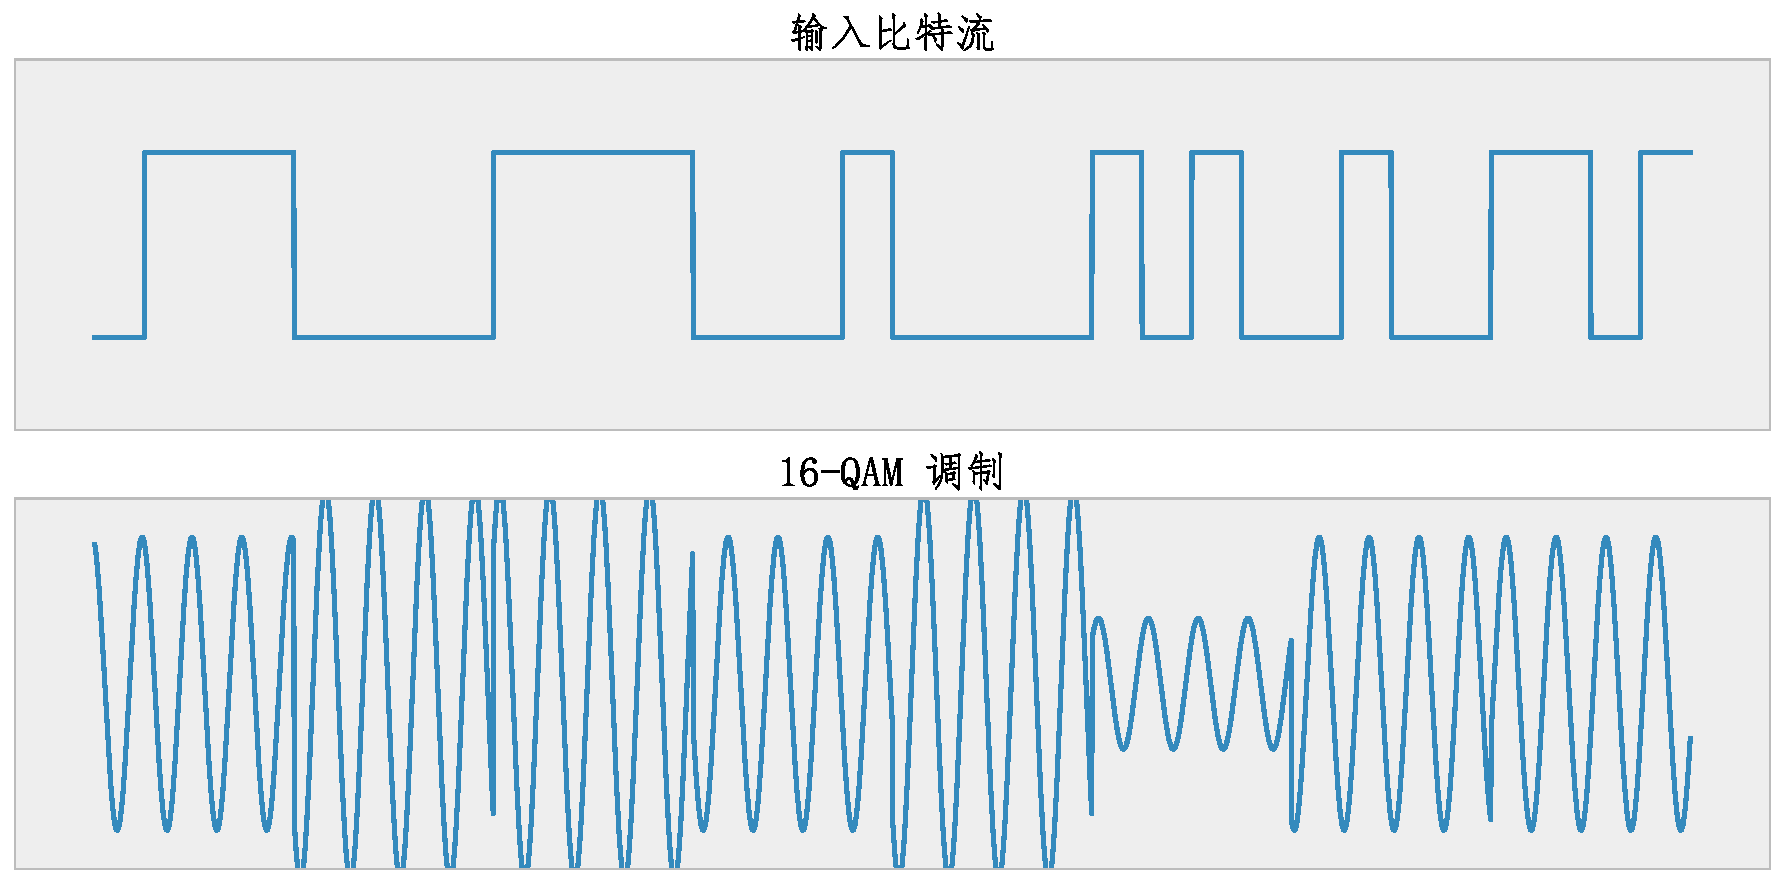
\includegraphics[width=\textwidth]{Image/qam.pdf}
    \caption{正交振幅调制示意图}
    \label{fig:QAM}
\end{figure}

% \dots

% \section{传统方法}\label{sec:background}
% 一般而言,AMR可以看作一种典型的模式识别问题,一般包含三个步骤,接收信号的预处理、特征提取和最后的调制分类。AMR任务的传统方法主要有两类:\textit{基于似然比(Likelihood Based)}的方法\cite{hameed2009likelihood}和\textit{基于特征提取(Feature Based)}的方法~\cite{hazza2013overview}。

% % 虽然基于似然的方法在贝叶斯意义上是最优的,但其通常需要较高的计算复杂性和对于调制信号的先验知识,这使得该方法对未知的信道环境十分敏感,从而影响了其适用性。基于特征提取的方法则受特征选取影响较大,不同的特征其识别结果也有很大的差别,因此如何选取特征 是识别结果好坏的关键。其次,由于特征提取需要花费一定的时间,这就导致了在实际 应用中也难以做到实时处理。~\cite{moser2015automatic}

% \subsection{似然比法}\label{sec:background}
% 基于似然比的方法将AMR视为多重假设检验问题~\cite{xu2010software},对不同的调制类型做出假设,并计算在不同假设下接收信号的似然比。然后,通过将似然比与预定义的阈值进行比较,确定接收信号的调制类型~\cite{dobre2007survey}。
% 似然比法是一种常见的统计方法,用于根据观测到的数据计算不同假设之间的似然比。在自动调制识别中,似然比法通常涉及计算信号的似然比值,然后选择具有最大似然比值的调制方式。当接收端获取到信号后,先对接收信号的未知目标参数进行建模,获取特定参数的概率分布,再根据特定的似然准则建立似然函数,计算每一个假设调制方式类型对应的似然值,最后根据贝叶斯信息准则(Bayesian Information Criterion, BIC),在一定阈值的约束下,选取最大似然值所对应的调制方式作为目标信号的预测调制方式。图~\ref{fig:likelihood}展示了似然比假设检验识别法的处理流程。

% \begin{figure}
%     \centering
%     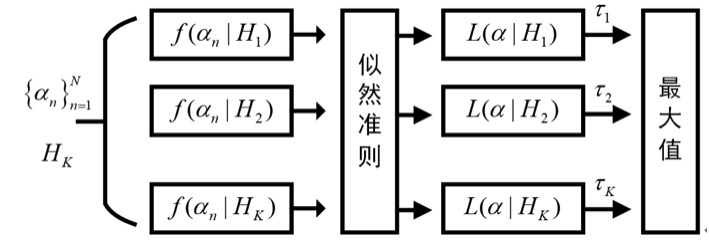
\includegraphics[width=0.8\textwidth]{Image/lb.jpg}
%     \caption{似然比法处理流程}
%     \label{fig:likelihood}
% \end{figure}
% 似然比法的不足:

% 对于复杂的信号模型,需要准确的先验知识,且在高维度空间中可能难以处理。

% 对噪声和非理想条件敏感,容易受到信噪比的影响。

% \dots

% \subsection{特征提取法}\label{sec:background}
% 特征提取法通过从信号中提取相关特征,如能量、频率分布和相位信息等,然后利用这些特征进行调制识别。其整个识别流程一般包括三个步骤,即信号预处理、特征提取和分类器识别,其中特征提取是关键步骤。信号预处理旨在通过对信号进行简单的变换,使其具有一定规范性,以降低后续数据处理的难度,例如对接收信号进行滤波和降频处理。同时,也需要对信号数据进行清洗和筛选,排除不合理的数据信息。特征提取的任务是在不同维度中寻找各种调制方式之间的差异。对于同一种调制方式,不同的特征反映出的调制信息也具有显著差异,其识别结果也存在一定的差异。因此,相较于基于统计模式的识别算法,选取适当的特征对于提高识别精度至关重要。图~\ref{fig:feature}展示了调制识别领域中常用的信号维度特征。

% \begin{figure}
%     \centering
%     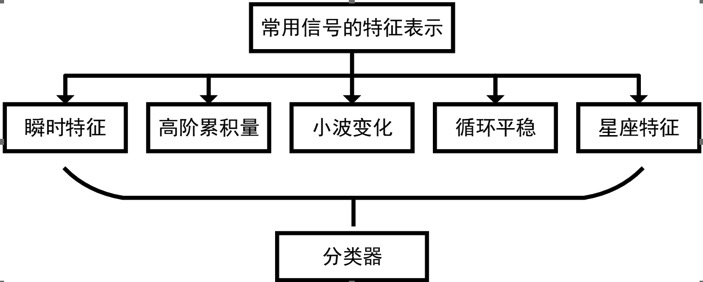
\includegraphics[width=0.8\textwidth]{Image/fb.jpg}
%     \caption{常用的信号维度特征}
%     \label{fig:feature}
% \end{figure}
% 特征提取法的不足:

% 依赖于手动设计的特征,可能无法适应复杂信号模式的变化。

% 难以处理大规模数据,且对特征选择的依赖可能导致信息丢失。

% \dot


\section{调制识别方法原理}\label{sec:background}

在自动调制识别领域,传统方法的研究进展主要集中在利用经典的信号处理技术和决策理论。这些方法通常依赖于从接收信号中提取特定的统计特征,如瞬时幅度、相位和频率等,来识别信号的调制类型。这些传统方法包括决策树、支持向量机(SVM)和人工神经网络等,它们在高信噪比(SNR)环境下能够实现较高的识别准确率。然而,这些方法在复杂的通信环境,如低信噪比或多径衰落条件下,性能往往受到限制。

传统的AMR方法主要依赖于特定的统计特征和经典的信号处理技术。这些方法在信噪比较高、环境相对稳定的情况下表现良好。然而,它们在处理复杂或低信噪比信号时的性能往往不足,且通常需要复杂的特征提取和大量的先验知识。
接下来介绍下似然比法的基本原理:

似然比法是一种经典的传统方法,长期以来一直是研究者们的关注焦点。似然比法基于统计决策理论,通过计算接收到的信号数据在不同假设调制类型下的似然比来实现调制类型的识别。这种方法的核心是利用接收信号的统计特性,结合已知调制类型的概率模型,估计信号的调制类型。

似然比法的工作原理建立在贝叶斯理论的基础上。该方法假设对于每一种可能的调制类型,信号都有一个相应的概率模型。这些概率模型描述了在特定调制类型下接收信号的统计特性。在实际应用中,似然比法通过计算每种调制类型下信号观测值的条件概率密度函数,并将其进行比较,从而确定最可能的调制类型。这一过程涉及到复杂的概率计算,尤其是在面对多种调制类型和大量数据时。

实施似然比法的过程主要包含以下几个步骤:首先,对于每一种可能的调制类型,建立一个相应的概率模型,通常是条件概率密度函数。然后,对于接收到的每个信号样本,计算在各种调制假设下的似然比。最后,选择具有最大似然比的调制类型作为识别结果。

似然比法在自动调制识别(AMR)中使用的核心公式是基于计算给定观测数据下不同调制类型的似然比。以下是似然比法中常用的一些基本公式及其简单介绍:

1. 似然函数:
    对于给定的观测数据 \( \mathbf{x} \) 和假设的调制类型 \( M \),似然函数定义为 \( L(\mathbf{x} | M) \),表示在调制类型 \( M \) 下观测到 \( \mathbf{x} \) 的概率。
\begin{align}
    L(\mathbf{x} | M) = p(\mathbf{x} | M),
\end{align}
    % \[ L(\mathbf{x} | M) = p(\mathbf{x} | M) \],
     其中 \( p(\mathbf{x} | M) \) 是在调制类型 \( M \) 下观测数据 \( \mathbf{x} \) 的条件概率密度函数。

2. 似然比:
   似然比是两种调制类型下似然函数的比值。对于两种假设的调制类型 \( M_1 \) 和 \( M_2 \),似然比定义为两者似然函数的比率。
\begin{align}
    \Lambda(\mathbf{x}) = \frac{L(\mathbf{x} | M_1)}{L(\mathbf{x} | M_2)},
\end{align}
%    \[ \Lambda(\mathbf{x}) = \frac{L(\mathbf{x} | M_1)}{L(\mathbf{x} | M_2)} \],
     这里 \( \Lambda(\mathbf{x}) \) 是似然比,用于比较两种调制类型的可能性。

3. 决策规则:
   在似然比法中,通过比较似然比与预先设定的阈值来做出决策。如果似然比超过阈值,选择一种调制类型;否则,选择另一种。
   如果 \( \Lambda(\mathbf{x}) > \text{阈值} \),选择 \( M_1 \);否则选择 \( M_2 \)。

似然比法的关键在于准确地估计条件概率密度函数 \( p(\mathbf{x} | M) \)。这通常涉及对信号模型的深入理解和复杂的数学运算。在实际应用中,由于通信信号的多样性和复杂性,这些概率密度函数的准确估计是似然比法中最具挑战性的部分。

似然比法在理想条件下能提供较高的识别准确率,这是因为它直接利用了信号的统计特性,并结合了精确的数学模型。这种方法在理论上具有坚实的基础,能够在信号质量良好时实现精确的调制类型识别。

然而,似然比法在实际应用中也存在一些明显的限制。最主要的挑战之一是计算复杂度高。由于需要进行大量的概率计算,特别是在多种调制类型和大数据量的情况下,这一方法的计算成本非常高。此外,似然比法对信噪比(SNR)非常敏感。在低信噪比或非理想信道条件下,其性能可能会显著下降。此外,该方法的性能依赖于对信号模型的精确知识,对模型假设的不准确可能导致识别性能下降。

尽管似然比法在理论上具有优势,并且在理想条件下可以实现较高的识别准确率,但它在实际应用中面临诸多挑战。这些挑战包括高计算复杂度、对低信噪比情况的敏感性以及对精确模型假设的依赖。因此,在现代通信系统中,研究者们开始探索其他方法,特别是那些能够更有效地处理复杂信号环境和大数据量的方法,如基于深度学习的AMR技术。随着计算能力的提升和算法的发展,深度学习方法在AMR领域显示出巨大的潜力,逐渐成为研究的新热点。尽管如此,似然比法作为一种经典的方法,在理论研究和特定应用场景中仍然具有重要价值。

特征提取方法是另一种常用的传统AMR方法。与似然比法不同,特征提取方法不直接利用信号的统计特性,而是通过从信号中提取特征来实现调制类型的识别。特征提取方法通常包含两个基本步骤:特征的选择和分类器的设计。特征选择的目的是从信号中提取最具代表性的特征,以实现最佳的识别性能。分类器的设计是为了将提取的特征与预先定义的调制类型进行匹配,从而实现调制类型的识别。

接下来将从信号特征的表示和分类器的设计两个方面介绍特征提取方法。

\textbf{(一)信号特征的表示}

1. 瞬时特征:
   瞬时幅度、相位和频率是分析调制信号中最基本的特征。瞬时幅度反映了信号强度的即时变化,瞬时相位提供了关于信号相位变化的信息,而瞬时频率揭示了信号频率随时间的变化情况。这些特征对于区分例如ASK(幅度键控)、FSK(频率键控)和PSK(相位键控)等基本调制类型非常有效。

2. 高阶统计特征:
   这类特征包括偏度和峰度,用于分析信号的分布形状和尾部特性。例如,高阶累积量如二阶和四阶矩可用于捕捉信号的非高斯特性。这些高阶统计特征对于识别复杂调制模式,如QAM(正交幅度调制)特别有用。

3. 变换域特征:
   变换域特征涉及将时间域信号转换到频域或其他域,例如通过傅里叶变换或小波变换。频域特征有助于理解信号的频率组成,特别是在频域中能量分布的特点。这对于识别频谱利用率和频谱效率高的调制类型尤为重要。

4. 星座图特征:
   星座图是调制信号在复平面上的图形表示,它为调制过程提供了直观的视图。通过分析星座图的形状、密度和分布,可以提取关于调制类型的重要信息。例如,不同的QAM调制在星座图上呈现不同的点分布模式。

5. 时频分布特征:
   时频分布特征提供了信号随时间变化的频率特性,适合于分析非平稳信号。通过分析时频分布,可以识别具有时间变化特性的复杂调制信号,这在现代通信系统中尤为重要。

\textbf{(二)分类器}

1. 支持向量机(Support Vector Machine, SVM):
   SVM是一种有效的分类算法,通过在特征空间中寻找最佳分割超平面来区分不同类别的数据。SVM特别适用于具有明显边界的分类问题。在AMR中,SVM可用于区分具有不同特征向量的调制类型。

2. 决策树:
   决策树通过从根到叶的顺序决策过程对数据进行分类。每个节点代表一个特征的决策点,根据该特征的值选择分支,直到到达叶节点,即分类结果。决策树易于理解和实现,适用于具有明显特征规则的调制类型识别。

3. 随机森林:
   随机森林是基于多个决策树构建的集成学习方法。它通过组合多个树的预测结果来提高分类的准确性和鲁棒性。在AMR中,随机森林能够有效处理大量的特征并提供稳定的分类结果。

4. 神经网络:
   神经网络,尤其是浅层神经网络,可用于特征提取法中的分类任务。它们通过学习特征与调制类型之间的非线性关系来进行分类。神经网络在处理复杂的调制识别问题时表现出色,尤其是当特征空间维度较高时。

5. K最近邻(K-Nearest Neighbor, KNN):
   KNN是一种基于邻近样本进行分类的简单方法。它根据最近邻样本的类别来决定新样本的类别。虽然KNN在小规模数据集上效果良好,但在大数据集上的计算成本较高。

特征提取法在AMR中的应用表明,有效的特征提取和精准的分类是提高调制识别性能的关键。随着通信技术的发展,尤其是在面对更复杂的信号和通信环境时,对于更先进的特征提取技术和更有效的分类算法的需求日益增长。

\subsection{传统方法的局限性}\label{sec:background}

在自动调制识别(AMR)的研究中,传统方法虽然在特定情况下表现良好,但它们也存在一些显著的缺陷,这限制了它们在复杂通信环境中的应用。这些局限性包括:

高计算复杂度:传统的AMR方法,特别是似然比法,涉及复杂的数学运算和概率计算,尤其是在多种调制类型和大数据量的情况下。这种高计算复杂度限制了其在实时或资源受限的应用中的可行性。

模型失配问题:传统方法往往依赖于对信号模型的精确假设。然而,在实际应用中,由于信道效应、噪声以及硬件限制等因素,实际信号可能与理论模型存在差异,导致模型失配。这种失配会显著降低识别准确率。

对特征提取的依赖:特征提取法的性能在很大程度上依赖于所选特征的有效性。不恰当或不充分的特征提取可能导致分类性能下降。此外,手动特征工程是一个复杂且耗时的过程,对先验知识和专业判断的依赖较大。

对信噪比的敏感性:在低信噪比或非理想信道条件下,传统AMR方法的性能可能会显著下降。这些方法对信号质量的依赖性限制了它们在复杂通信环境下的应用。

\subsection{深度学习方法}\label{sec:background}
近年来,深度学习技术为AMR带来了革命性的改变。深度学习模型,特别是卷积神经网络(Convolution Neural Network, CNN)和循环神经网络(Recurrent Neural Network, RNN),已经被证明在从原始信号中直接提取特征和执行复杂的分类任务方面非常有效。这些模型能够在多种条件下实现高准确率的调制识别,即使在低信噪比或非理想信道条件下也是如此。尽管如此,深度学习方法在处理AMR问题时仍面临诸如训练数据需求量大、模型复杂度高以及对低信噪比情况下性能的提升等挑战。接下来将详细介绍主要的深度学习模块及其在调制识别问题中的优势:

1.卷积神经网络(CNN)是深度学习中的基础模型之一,特别适用于处理具有空间结构的数据。CNN通过其多层卷积结构能够从原始I/Q数据中自动提取特征,无需复杂的特征工程。CNN的每一层都能捕获信号的不同层次特征,而池化层则用于降低特征的维度和复杂性,增强模型的泛化能力。在调制识别中,CNN的主要优势在于其强大的特征提取能力,使其能够适应不同的调制类型,即使在低信噪比环境下也能保持较好的性能。

2.循环神经网络(RNN)和长短期记忆网络(LSTM)是处理时间序列数据的理想选择,能够有效捕捉数据中的时间依赖性。RNN通过其循环结构捕获时间序列中的信息,适用于处理时间相关的信号特性。LSTM引入了遗忘门和输入门,能够有效地处理长期依赖问题,避免了RNN中的梯度消失问题。在AMR中,RNN/LSTM的优势在于它们能够处理信号的时序特征,尤其适用于识别那些具有复杂时间结构的调制类型。

3.注意力机制是一种使模型能够聚焦于输入数据中最重要部分的技术,能够提高模型对关键信息的敏感性。注意力机制使模型能够识别并集中处理输入数据的关键部分,提高处理效率和准确性。在调制识别应用中,注意力机制尤其有用于识别那些在特定时间窗口或频率范围内具有显著特征的信号类型。它能够帮助模型集中处理最关键的信号部分,提高识别准确率。

总体而言,深度学习方法为AMR提供了一种高效且强大的替代方案。这些方法能够直接从原始信号中自动提取特征,并有效地处理各种调制类型。CNN的特征提取能力、RNN/LSTM的时间依赖性处理能力以及注意力机制的关键信息聚焦能力,使它们在处理复杂的调制识别问题时表现出色。随着技术的不断发展,深度学习方法有望在AMR领域中发挥越来越重要的作用,特别是在应对复杂通信环境和高动态信号条件下的挑战。

\subsubsection{宽带信号调制识别}\label{sec:background}

宽带信号调制识别在自动调制识别领域中呈现出独特的挑战,主要由于其涉及的频率范围广泛且信号特性复杂。从采样角度来看,宽带信号的处理面临着存储和设备成本的重大挑战。传统的采样方法按照奈奎斯特定理要求,采样频率必须至少是信号最高频率的两倍,这在宽带信号的情况下导致了极高的采样率。高采样率随之带来的数据量巨大,不仅需要大量存储空间,而且对数据处理提出了高要求,增加了数据处理的复杂性。此外,实现这种高速采样的设备往往昂贵,限制了宽带信号处理技术的普及。

为了克服这些挑战,亚采样(本研究中选取多陪集采样)技术应运而生。亚采样技术允许以低于奈奎斯特速率的采样频率对信号进行采样,从而减少了所需的存储空间和处理能力,降低了设备成本。通过采用特定的采样策略和后续的信号处理算法,可以从低速率采样的数据中恢复出原始信号的关键信息。

在宽带信号识别方面,自动调制识别的研究相对较少,但随着宽带通信技术的发展,对于这方面的研究需求正在迅速增长。在宽带信号的处理中,自动调制识别不仅需要识别信号的调制类型,还需要确定信号占用的子带位置。这增加了自动调制识别的复杂性,因为宽带信号涉及更广泛的频率范围和更复杂的信号特性。亚采样技术在这里发挥着关键作用,它通过降低采样率,使得对宽带信号的处理变得更为可行和经济。

然而,亚采样技术也带来了新的挑战,尤其是在信号重构和调制类型识别方面。如何从低速率采样的数据中准确地恢复出信号的关键特征,并进行有效的调制识别,是当前研究的重点。这需要创新的信号处理算法和先进的数据分析技术,以从有限的采样数据中提取出足够的信息进行准确的调制识别。

目前,针对宽带信号的自动调制识别技术仍处于发展阶段,需要更多的研究来解决宽带环境下的特定挑战,特别是在信号重构和调制类型识别的准确性方面。未来的研究可能会集中在开发新的亚采样技术和相关的信号处理算法,以提高宽带信号处理的效率和准确性。同时,随着深度学习等先进技术的应用,有望在提高宽带信号自动调制识别性能方面取得重要进展。

总体而言,自动调制识别领域的研究正在从传统方法向深度学习方法转变,每种方法都有其独特的优势和局限性。随着通信技术的不断发展,特别是宽带通信技术的兴起,自动调制识别技术面临着新的挑战和机遇。未来的研究需要关注在复杂环境下提高自动调制识别性能的方法,尤其是在处理宽带信号方面的进展和挑战。


\section{深度学习理论基础}\label{sec:background}

神经网络的基本结构由输入层、隐藏层和输出层构成,它们通过带权重的连接相互作用。在深度学习中,这些层可以堆叠起来形成深度神经网络,以学习输入数据中的复杂模式和特征。每一层都由若干神经元组成,其中每个神经元负责对输入数据进行一定的数学变换。这些变换通常涉及到权重(\(W\))和偏置(\(b\))的线性组合,随后通过一个非线性的激活函数(\(f\))进行处理。这种结构使得神经网络能够逼近几乎任何复杂的函数。
神经网络由多层神经元组成,每层神经元可以接收上一层神经元的输出作为输入,并产生输出到下一层。一个基本的三层神经网络可以表示为:

\begin{equation}
    y = f(W_2 f(W_1 x + b_1) + b_2)
\end{equation}

其中,\( x \) 是输入向量,\( W_1 \) 和 \( W_2 \) 是权重矩阵,\( b_1 \) 和 \( b_2 \) 是偏置向量,\( f \) 是激活函数,\( y \) 是输出向量。在这种结构中,\( W_1 \) 和 \( b_1 \) 对应于第一层(通常称为隐藏层)的权重和偏置,而 \( W_2 \) 和 \( b_2 \) 对应于第二层(输出层)的权重和偏置。激活函数 \( f \) 用于引入非线性,使得网络能够学习和模拟非线性关系。

每一层的神经元数量和层的总数可以根据特定的应用和数据集进行调整。隐藏层的深度和宽度(即每层的神经元数量)是神经网络设计中的关键参数,它们直接影响到网络的能力和复杂度。理论上,增加更多的隐藏层和神经元可以使网络能够学习更复杂的函数,但这也会增加训练的难度和过拟合的风险。

在训练过程中,通过反向传播算法和梯度下降等优化方法调整权重和偏置,以最小化网络输出和真实标签之间的差异。这个过程涉及到计算损失函数(如均方误差或交叉熵损失)相对于网络参数的梯度,并根据这些梯度更新参数。

神经网络的这种层级结构和训练机制使其成为一种强大的工具,能够应用于广泛的任务,包括图像识别、语音识别、自然语言处理等领域。通过调整网络结构和参数,研究人员和工程师能够设计出适应特定问题的模型,解决传统算法难以处理的复杂任务。

\subsection{激活函数}\label{sec:background}
激活函数用于引入非线性,使得神经网络可以学习并表示复杂的函数。常见的激活函数包括:

\subsubsection{Sigmoid函数}
Sigmoid函数是一个常用的激活函数,它的数学表达式如公式\ref{eq:sigmoid}所示:
\begin{equation}
    \sigma(x) = \frac{1}{1 + e^{-x}}
    \label{eq:sigmoid}
\end{equation}
\begin{figure}
    \centering
    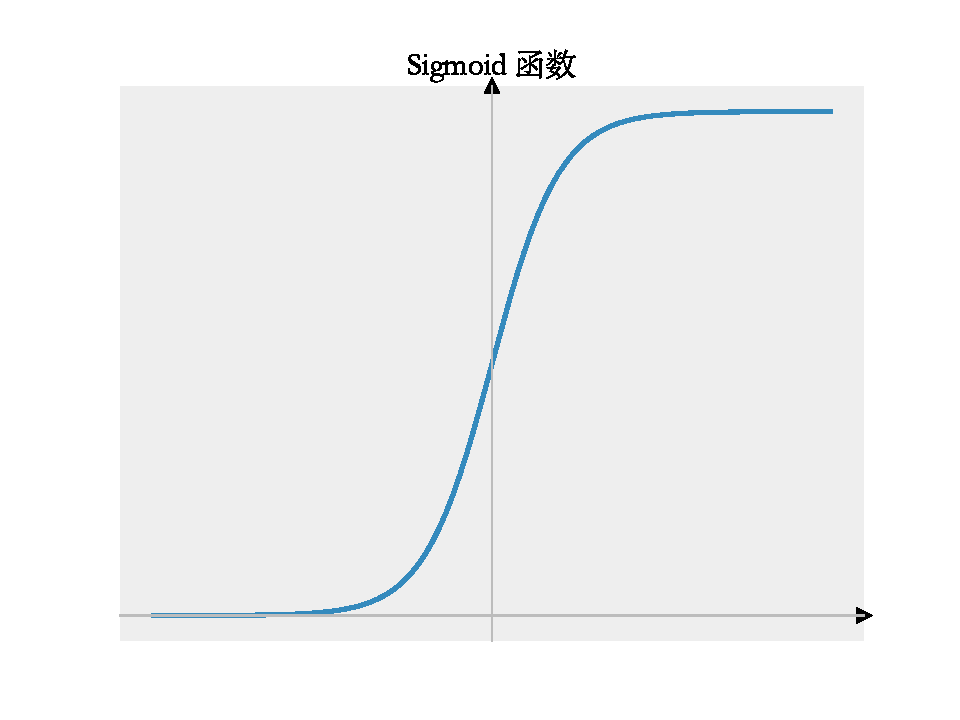
\includegraphics[width=0.8\textwidth]{Image/sigmoid.pdf}
    \caption{Sigmoid函数}
    \label{fig:sigmoid}
\end{figure}

Sigmoid函数是一个在机器学习和深度学习领域广泛应用的非线性函数。其特征在于将任意实数值映射到(0, 1)区间内,使其能够表示概率、进行二分类等。函数图形呈S形曲线,如图像\ref{fig:sigmoid}所示,因而得名Sigmoid(即“S形”的意思)。

Sigmoid函数的取值范围限定在(0, 1)之间,这一性质使其尤为适用于需要输出概率预测的场合,如二分类问题的概率输出。数学上,当输入值x趋向于正无穷时,\( \sigma(x) \)趋近于1;当x趋向于负无穷时,\( \sigma(x) \)趋近于0。正是由于这种平滑的过渡特性,Sigmoid函数能够在模型中充当激活函数,将线性输入转换为非线性输出,为神经网络模型提供必要的非线性特性,使得网络能够学习和模拟复杂的函数映射关系。

然而,Sigmoid函数也存在一些局限性,如梯度消失问题,即当输入值处于饱和区(即极大或极小值附近)时,其梯度接近于零,导致在这些区域内,参数更新缓慢,影响模型的学习效率。尽管如此,由于其形式简单、易于理解,Sigmoid函数在早期的神经网络研究中扮演了重要角色,并为后续的激活函数设计提供了基础。


\subsubsection{ReLU函数}
ReLU(Rectified Linear Unit,修正线性单元)函数是一种在深度学习模型中广泛使用的激活函数,数学表达式如公式\ref{eq:relu}所示:
\begin{equation}
    \text{ReLU}(x) = \max(0, x)
    \label{eq:relu}
\end{equation}
\begin{figure}
    \centering
    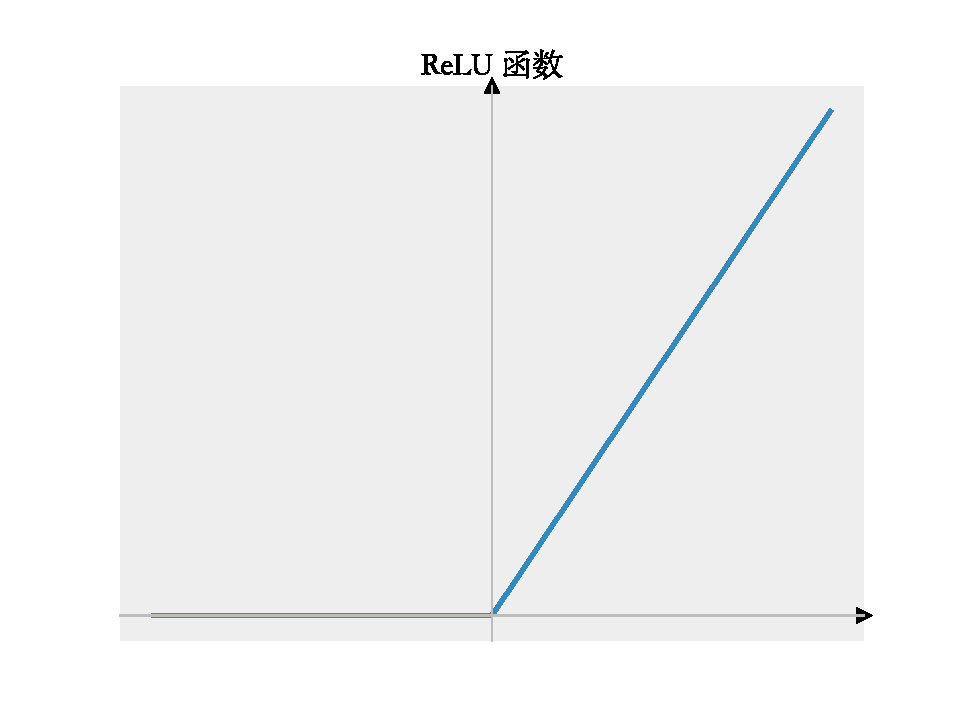
\includegraphics[width=0.8\textwidth]{Image/relu.pdf}
    \caption{ReLU函数}
    \label{fig:relu}
\end{figure}

该函数的特点是对于所有正数输入保持线性,而对于负数输入则输出为零。ReLU函数的图形表现为一个折线,如图像\ref{fig:relu}所示,其中$x>0$时,函数输出等于输入;$x≤0$时,输出恒为0。

ReLU函数因其计算简单、梯度传播效率高而受到广泛欢迎。在正数区域,ReLU的梯度恒为1,这一性质有利于减轻深度神经网络训练过程中的梯度消失问题,相比之下,Sigmoid函数和Tanh函数在输入值绝对值较大时梯度接近于零,容易引发梯度消失问题。此外,ReLU激活函数还能够通过其非饱和的性质促进神经网络中稀疏激活的产生,有助于提高网络的表达能力和计算效率。

然而,ReLU函数也有其局限性,其中最著名的是“死亡ReLU”问题。这是指在网络训练过程中,一旦某个神经元的输入在训练过程中始终为负数,则该神经元的输出始终为0,导致相应参数不再更新,这样的神经元被称为“死亡”神经元。为了克服这一问题,研究人员提出了多种ReLU的变体,如Leaky ReLU、Parametric ReLU等,这些变体试图保留ReLU在正区间的线性特性,同时为负区间的输入提供一个小的、非零的梯度,以促进全面的参数更新。

尽管存在上述问题,但得益于其简洁性和效率,ReLU及其变体仍然是当前深度学习领域最为流行和有效的激活函数之一。

\subsubsection{Tanh函数}
Tanh(双曲正切)函数是一种常用的激活函数,其数学表达式如公式\ref{eq:tanh}所示:
\begin{equation}
    \tanh(x) = \frac{e^x - e^{-x}}{e^x + e^{-x}}
    \label{eq:tanh}
\end{equation}
\begin{figure}
    \centering
    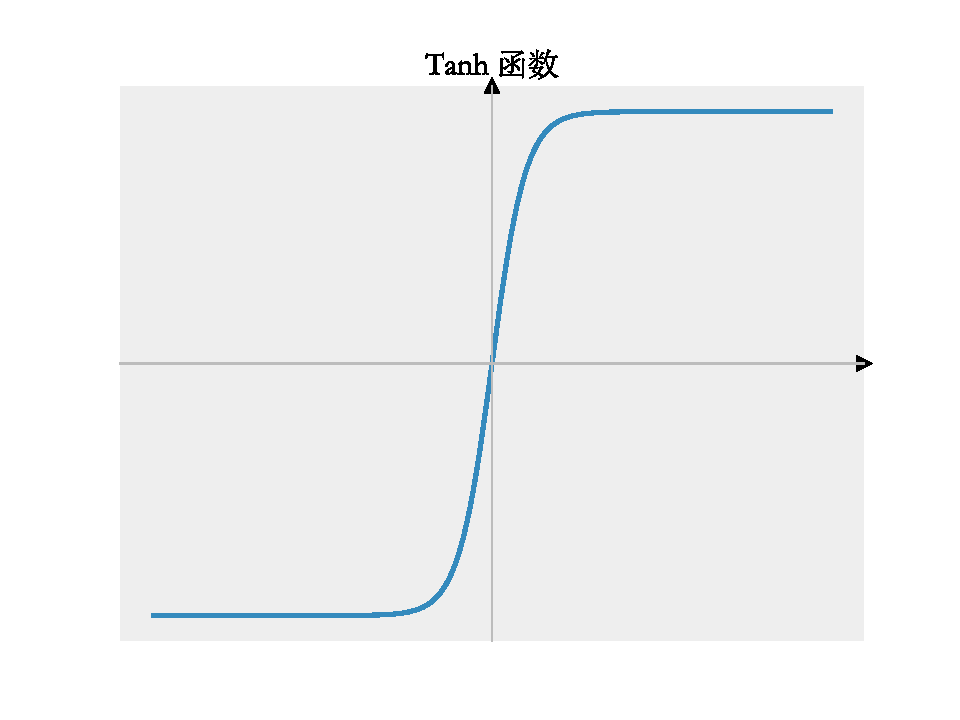
\includegraphics[width=0.8\textwidth]{Image/tanh.pdf}
    \caption{Tanh函数}
    \label{fig:tanh}
\end{figure}
与Sigmoid函数类似,Tanh函数也是一种S形的非线性激活函数,如图\ref{fig:tanh}所示,但其输出范围是(-1, 1),这一点与Sigmoid函数的输出范围(0, 1)有所不同。Tanh函数在输入值为0时输出0,其对称性有助于数据的中心化,这通常能够加快收敛速度,改善学习效率。

Tanh函数的主要优点之一是其输出范围,因为它能够输出负值,所以在处理以0为中心的数据时比Sigmoid函数表现更好。这种以0为中心的性质使得Tanh函数在一些场合下比Sigmoid函数更受青睐,特别是在隐藏层的激活函数选择上。在神经网络的训练过程中,Tanh函数能够有效地控制正向和反向传播时梯度的大小,从而避免了Sigmoid函数中可能出现的梯度消失问题。

然而,尽管Tanh函数比Sigmoid函数具有更好的性能,它仍然不能完全避免梯度消失的问题,特别是在处理深层网络时。当输入的绝对值很大时,Tanh函数的梯度也会接近于零,这会导致深层网络在训练过程中更新速度缓慢。

尽管存在这些局限性,Tanh函数由于其输出范围和性能,依然是深度学习领域中常用的激活函数之一,尤其适用于要求输出为双向的场合,如一些特定的神经网络架构中。随着深度学习领域的发展,Tanh函数和其他激活函数一样,根据特定的应用场景和网络架构被灵活选用,以达到最优的模型性能。

\subsection{反向传播算法}\label{sec:background}
反向传播算法是深度学习中最核心的概念之一,它允许网络通过梯度下降法高效地调整其参数,以最小化损失函数。这一过程涉及到对网络中每一层逐层反向计算梯度,并根据这些梯度更新相应的参数。对于一个简单的两层网络,参数更新可以表示为:

\begin{equation}
    W = W - \eta \frac{\partial \mathcal{L}}{\partial W}
\end{equation}

其中,\(W\) 是权重矩阵,\(\eta\) 是学习率,\(\mathcal{L}\) 是损失函数。

深度神经网络的训练分为两个阶段:前向传播和反向传播。在前向传播阶段,输入数据沿着网络前进,通过每一层的加权和及激活函数处理,最终产生输出。这一过程中,每一层的输入和输出都被存储起来,以便之后的梯度计算。

在反向传播阶段,算法从输出层开始,逆向通过网络,计算每一层的梯度。这一过程利用链式法则,根据损失函数相对于网络参数的偏导数来计算梯度。具体来说,对于每一层,损失函数的梯度可以表示为该层输出对损失的影响和该层输入对其输出的影响的乘积。

梯度计算完成后,参数更新规则被用来调整网络中的权重和偏置,以减少预测值和实际值之间的差异。这一更新过程可以通过多种优化算法来实现,如随机梯度下降(SGD)、Adam或RMSprop等。

反向传播算法的成功部分在于其能够有效地计算网络中所有参数的梯度,即使在网络结构非常复杂时也是如此。这使得神经网络能够通过学习过程自动调整其参数,从而在各种任务中实现优秀的性能。此外,反向传播算法的效率和普适性使其成为训练深度学习模型的基石之一。
\subsection{损失函数}\label{sec:background}
损失函数在神经网络中扮演着至关重要的角色,它量化了模型输出与真实标签之间的差异。选择合适的损失函数对于训练有效的神经网络模型是非常关键的。常见的损失函数有均方误差(MSE)和交叉熵损失,它们分别适用于回归问题和分类问题。

\subsubsection{均方误差(MSE)} 
均方误差是最常用的回归损失函数,定义为预测值与真实值之差的平方和的平均值。数学表达式为:
\begin{equation}
    \mathcal{L}_{\text{MSE}} = \frac{1}{n} \sum_{i=1}^{n} (y_{\text{pred}, i} - y_{\text{true}, i})^2
\end{equation}
其中,\(y_{\text{pred}, i}\) 是第\(i\)个样本的预测值,\(y_{\text{true}, i}\) 是对应的真实值,\(n\) 是样本总数。

\subsubsection{交叉熵损失(Cross-Entropy Loss)}
交叉熵损失是处理分类问题时最常用的损失函数之一,特别是在二分类和多类分类问题中。它衡量的是实际输出的概率分布与预测输出的概率分布之间的差异。对于二分类问题,交叉熵损失的数学表达式为:
\begin{equation}
    \mathcal{L}_{\text{CE}} = -\sum_{i=1}^{n} [y_{\text{true}, i} \log(y_{\text{pred}, i}) + (1 - y_{\text{true}, i}) \log(1 - y_{\text{pred}, i})]
\end{equation}
对于多类分类问题,其表达式稍有不同,但核心概念保持一致,即最小化真实标签和预测概率之间的差异。

通过精心设计的损失函数,可以引导神经网络在训练过程中不断调整参数,以期望输出更接近于真实标签。损失函数的选择依赖于特定的任务(如回归或分类)和所需的性能指标。


\section{宽带信号模型}\label{sec:background}


宽带信号的模型是现代通信系统中一个重要的概念,其特点是包含多个子带信号,这些子带信号经过不同频率的频移后叠加在一起。下面是对宽带信号模型的数学表述及其关键假设的进一步阐述。

\subsection{宽带信号的数学模型}\label{sec:background}
宽带信号的数学表达式可以表示为:
\begin{equation}
    y(t)=\sum_{i=1}^N h_i(t) \ast a_i(t)e^{j2\pi f_i t}+\eta(t),
\end{equation}
其中,\( \ast \) 表示卷积操作,\( N \) 是子带的数量,\( h_i(t) \) 是第 \( i \) 个信道的冲激响应,\( a_i(t) \) 是第 \( i \) 个信道的子带信号,\( f_i \) 是第 \( i \) 个信道的子带频率,而 \( \eta(t) \) 表示加性噪声,通常假定为加性白高斯噪声(AWGN)。

经过调制的子带信号 \( a_i(t) \) 可以表示为:
\begin{equation}
    a_i(t)=\sum_{l=1}^L g(t-lT_s)b(l),
\end{equation}
其中,\( g(t) \) 是基带脉冲成形滤波器的脉冲响应,用于在保持符号间干扰(ISI)最小化的同时最大化信号带宽的效率。\( T_s \) 是符号持续时间,\( b(l) \) 是第 \( l \) 个时间步长的比特值。

\subsection{假设条件}\label{sec:assumptions}
为了适应实际通信场景,对宽带信号模型引入了以下两个关键假设:

\textbf{假设1:}宽带信号 \( y(t) \) 的采样频率 \( F_s \) 足够高,以覆盖所有子带信号的总带宽。具体来说,\( F_s \) 大于或等于 \( N \) 个子带信号带宽 \( B \) 之和,即 \( F_s \geq NB \)。这一假设确保了采样后的信号能够准确地表示原始的宽带信号。

\textbf{假设2:}任何带宽超过 \( B \) Hz 的子带信号可以被视为多个带宽小于 \( B \) Hz 的子带信号的组合。这一假设简化了宽带信号的处理,使其成为对多个窄带信号处理的扩展。

以上模型和假设为理解和处理宽带信号提供了一个清晰的框架。通过将宽带信号分解为多个子带信号,并考虑其采样频率和带宽特性,我们能够更加有效地分析和处理这些信号。这对于开发高效的宽带信号处理算法,特别是在调制识别和解调方面,至关重要。



\section{压缩感知理论基础}\label{sec:background}

压缩感知理论借助信号在时域、频域或其他变换域中的稀疏特性或可压缩性,通过低于奈奎斯特速率的采样率对信号进行压缩采样。最终,通过解决一个欠定线性方程组,运用适当的信号重建算法对信号进行还原。具体而言,经典的压缩感知问题可以用如下方程描述:

\begin{equation}
    y=Ax,
\end{equation}

其中,$x \in \mathbb{R}^n$ 表示待采样的原始信号,$y \in \mathbb{R}^m$ 为采样信号,$A \in \mathbb{R}^{m \times n}$是一个 $m \times n$ 的观测矩阵,通常满足 $m < n$。在这种情况下,上述方程是欠定的,存在无数个满足要求的解。压缩感知的目标在于从这无数个解中找到最稀疏的解,即具有最少非零元素的解。

对压缩感知系统性能的影响主要涉及三个方面的理论基础。首先是信号的稀疏表示,其要素在于通过适当的变换域表达信号的稀疏性或可压缩性。其次是压缩采样,即以低速采样率对信号进行压缩,从而有效减少采样数据量。最后是信号重建,其中通过适当的信号重建算法解决欠定线性方程组,找到最优的原始信号重建。

\subsection{信号的稀疏表示}

信号的稀疏特性指的是该信号能够被表示为少数个特征向量的线性组合,因此该信号仅包含有限数量的非零元素。然而,自然信号在时域上通常不具备稀疏性质,但在某些变换域下可能表现出稀疏性质。因此,信号的稀疏表示成为压缩感知研究的关键前提和理论基础,同时也是信号重建的重要先验知识。对于大多数不具备稀疏特性的信号,可以通过应用某个变换域,使其呈现出稀疏性质,从而进行信号的压缩采样和重建研究。这一过程充分利用了信号在不同表示下的稀疏性,为有效的信号采样和重建提供了理论支持。

考虑一个n维列向量信号 $x \in \mathbb{R}^n $,将其在某个变换域上进行稀疏变换表示为:

\begin{equation}
    x = \phi s,
\end{equation}

其中 $\phi \in \mathbb{R}^{n \times n}$ 表示稀疏变换矩阵, $s \in \mathbb{R}^n$ 表示原始信号 $x$ 在该变换域上的稀疏向量。这个稀疏向量 $s$ 描述了原始信号 $x$ 在所选变换域上的稀疏程度。在这种表示下,通过矩阵 $\phi$ 的作用,信号 $x$ 被表达为在所选变换域上的稀疏向量 $s$ 的线性组合。这一表示为信号在压缩感知中的采样和重建提供了基础,使得原始信号的信息可以更有效地被稀疏向量 $s$ 所表示。

常见的稀疏变换域包括频域、小波域等。在本文中,我们讨论的是频域上具有稀疏特性的宽带信号。具体而言,它指的是信号在频域上仅存在有限个较大的数值,而其他频率上的数值相对较小,可以被视为可以忽略的部分。这种频域上的稀疏性意味着信号主要集中在少数几个频率分量上,为压缩感知提供了可利用的特性。

在频域上的稀疏特性通常对于宽带信号是一种普遍现象,其中仅有限个频率成分对整个信号的能量贡献显著,而其他频率分量相对较弱。这种信号在频域上的特性为通过适当选择变换域来实现信号的稀疏表示提供了可能性,进而为压缩感知的应用提供了有利的条件。在这一背景下,选择适当的频域变换,例如傅里叶变换,可以有效地捕捉到信号在频域上的稀疏性质,为信号的压缩采样和重建奠定了基础。

\subsection{多陪集采样}

多陪集采样是一种周期性的非均匀亚奈奎斯特采样技术,旨在实现对连续时间频谱稀疏信号的压缩采样。该采样结构由多个分支组成,每个分支由一个延时单元和一个低速ADC转换器构成。每个延时单元对输入信号施加不同程度的时延,从而在时间上形成分支之间的周期性延时差异。整个采样框架的结构如图~\ref{fig:multicoset}所示。

对于输入的宽带信号 \(x(t)\),首先在时刻 \(t = (mL + c_i)T, i = 1,2,\ldots,p, m \in \mathbb{Z}\) 进行非均匀采样,得到离散采样序列。其中,\(T\) 表示输入宽带信号的奈奎斯特采样时间周期间隔。与奈奎斯特采样定理相比,多陪集采样的周期间隔为奈奎斯特采样的 \(L\) 倍,因此其采样频率降低为奈奎斯特采样频率的 \(1/L\)。

\begin{figure}
    \centering
    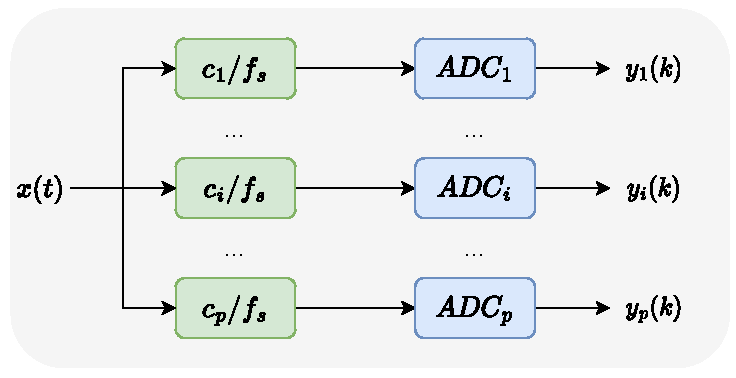
\includegraphics[width=0.8\textwidth]{Image/multi_coset.pdf}
    \caption{多陪集采样示意图}
    \label{fig:multicoset}
\end{figure}

集合 \(C = \{c_i\}_{i=1}^p\) 表示从集合 \(\{0,1,\ldots,L-1\}\) 中选择的 \(p < L\) 个不同的整数,这些整数构成了多陪集采样的模式。在多陪集采样中,选择了这些不同的整数作为时延,从而在时域上对输入信号进行了非均匀采样。这种方式的采样频率降低,有助于减少采样数据量,特别适用于宽带信号,其中信号的频谱不是均匀分布,而是集中在某些频率分量上。通过选择适当的 \(C\) 和 \(L\),可以灵活地调整采样方式,以满足信号的频谱特性和采样资源的限制。

\begin{figure}
    \centering
    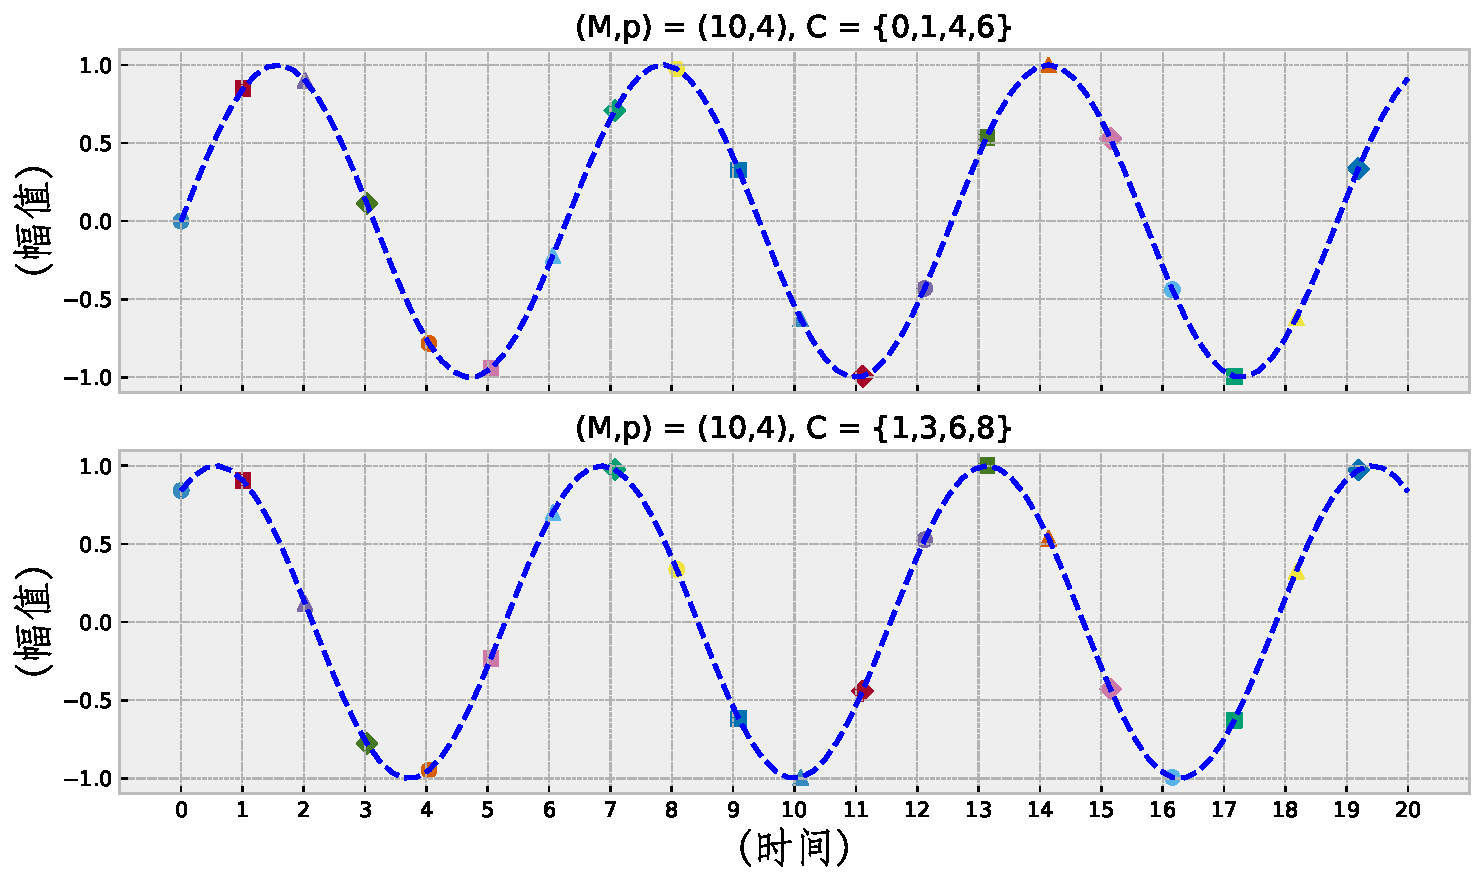
\includegraphics[width=\textwidth]{Image/mcs_process.pdf}
    \caption{多陪集采样过程示意图}
    \label{fig:multicoset_sample}
\end{figure}

图~\ref{fig:multicoset_sample}展示了多陪集采样的采样示意图,其中采样周期 \(M = 10\),采样通道数 \(p = 4\),并呈现了两种不同的采样模式,分别为 \(C = \{0,1,4,6\}\) 和 \(C = \{1,3,6,8\}\)。

在图中,圆形表示第一通道的采样点,三角形表示第二通道的采样点,正方形表示第三通道的采样点,菱形表示第四通道的采样点。通过观察图示,可以发现多陪集采样采用了一种与传统奈奎斯特采样方式不同的周期非均匀采样技术。采样模式的选择通过集合 \(C\) 中的不同整数,导致了在时域上的不同时延,形成了非均匀的采样结构。

这种多陪集采样技术的优势在于能够以较低的采样频率有效地采样宽带信号,同时通过灵活选择采样模式,适应信号频谱的稀疏性质。这样的非均匀采样方式为在资源受限的情况下实现对宽带信号的高效采样和重建提供了一种有益的途径。

\section{数据集}\label{sec:background}

% \begin{table}[htbp]
%     \centering
%     \caption{数据集概览}
%     \resizebox{\textwidth}{!}{%
%         \begin{tabular}{cm{0.4\linewidth}ccccm{0.2\linewidth}m{0.25\linewidth}}
%             \toprule
%             数据集 & 调制模式 & 样本维度 & 数据集大小 & 信噪比范围 & 特点 & 适用任务 \\
%             \midrule
%             RadioML 2016.10A & 11 类 (8PSK, BPSK,  CPFSK, GFSK, PAM4, AM-DSB, AM-SSB, 16QAM, 64QAM, QPSK, WBFM) & 2 \times 128 & 220000 & -20:2:18 & 短序列调试分类 & 传统方法与深度学习方法性能比较 \\
%             \midrule
%             RadioML 2016.10B & 10 类 (8PSK, BPSK,  CPFSK, GFSK, PAM4, AM-DSB,
%             16QAM, 64QAM, QPSK, WBFM) & 2 \times 128 & 1200000 & -20:2:18 & 短序列调制分类  (数据集更大) & 传统方法与深度学习方法性能比较 \\
%             \midrule
%             RadioML 2018.01A & 24类(OOK, 4ASK, 8ASK, BPSK, QPSK, 8PSK, 16PSK, 32PSK, 16APSK, 32APSK, 64APSK, 128APSK, 16QAM, 32QAM, 64QAM, 128QAM, 256QAM, AM-SSB-WC, AM-SSB-SC, AM-DSB-WC, AM-DSB-SC, FM, GMSK, OQPSK) & 2 \times 1024 & 2555904 & -20:2:30 & 长序列调制分类  (可模拟亚采样任务) & 可用于多种深度学习任务(调制识别、信号重构等) \\
%             \midrule
%             GBSense 2022 Basic & 13类(APSK16, APSK32, APSK64, ASK8, BPSK, OQPSK, PSK16, PSK8, QAM128, QAM16, QAM256, QAM64, QPSK) & 16 \times 1024 & 124800 & 真实环境采集信号 &欠采样宽带信号(单用户)调制分类 & 深度学习模型性能验证 \\
%             \midrule
%             GBSense 2022 Advance & 同上 & 16 \times 1024 & 102400 & 真实环境采集信号 &欠采样宽带信号(多用户)调制分类 & 多任务(包括宽带频谱感知与子带调制识别)深度学习模型性能验证 \\
%             \midrule
%             GBSense 2023 Basic & 2类(8PSK, 16QAM) & 16 \times 20 & 138240 & 真实环境采集信号 &欠采样宽带信号(单用户)调制解调 & 多任务深度学习解调(一个样本对应一个信息) \\
%             \midrule
%             GBSense 2023 Advance & 3类(QPSK, 8PSK, 16QAM) & 16 \times 20 & 500000 & 真实环境采集信号 &欠采样宽带信号(多用户)调制解调 & 多任务深度学习解调(一个样本对应多个信息)\\
%             \bottomrule
%         \end{tabular}
%     }
%     \label{tab:dataset}
% \end{table}

% 本研究使用多个开源数据集,包括由GNURadio生成的RadioML 2016.10A/B和RadioML 2018.01A,以及通过多陪集采样获取的真实宽带信号数据集GBSense 2022 Basic/Advance,以及专为解调任务设计的GBSense 2023 Basic/Advance。这些数据集为后续实验提供了可靠的基础支持。表~\ref{tab:dataset}简单介绍了这些数据集的基本信息。


% 当前,主流的AMR研究倾向于采用RadioML2016.10a数据集。该数据集数据量适中,包含一些常见的模拟和数字调制类型,如QAM、PSK、FSK和AM等。该数据集的采样点数适中,数据集大小也相对较小,适合用于验证算法的有效性。一般可用于传统算法和较为轻量的深度学习算法之间的性能比较。后续的RadioML 2016.10b数据集是对RadioML 2016.10a数据集的扩展,数据集大小更大,更适用于研究深度学习算法的鲁班性和泛化能力。而RadioML 2018.01a数据集则更为庞大,包含了24种调制类型,采样点数也增至1024,更能模拟真实环境中所采样到的信号,适用于更复杂的深度学习算法研究。

% GBSense 2022 Basic数据集通过多陪集采样获取真实宽带信号数据,包含13种调制类型,采样点数为1024,使用了8个低速的ADC进行采样,每个ADC的时延分别为16、11、1、0、27、24、37、31。各采样同一信号的同相分量和正交分量,故最终采样的信号维度为$16 \times 1024$。该数据集适用于研究亚采样宽带信号的调制识别问题。GBSense 2022 Advance数据集的采样方式与GBSense 2022 Basic相同,但采样的信号为多用户的宽带信号,即所采样的信号为多个用户的信号叠加。具体的任务是识别每个用户的调制类型及其所占的子带编号。

% GBSense 2023数据集的基本形式类似于GBSense 2022,不过其任务是对欠采样的宽带信号进行解调。相较于调制识别任务,解调任务需要识别信号的调制类型和符号长度等。在Advance版本中还需要对子带编号进行识别,因此其难度更大,同时对该任务的研究更具有实际意义。

\begin{table}[htbp]
    \centering
    \caption{数据集概览}
    \resizebox{\textwidth}{!}{%
        \begin{tabular}{m{0.3\linewidth}m{0.35\linewidth}m{0.2\linewidth}m{0.2\linewidth}m{0.15\linewidth}m{0.3\linewidth}}
            \toprule
            数据集 & 调制模式 & 样本维度 & 数据集大小 & 信噪比范围 & 适用任务 \\
            \midrule
            RadioML 2016.10A \\ (短序列) & 11 类 (8PSK, BPSK, CPFSK, GFSK, PAM4, AM-DSB, AM-SSB, 16QAM, 64QAM, QPSK, WBFM) & 2 \times 128 & 220000 & -20:2:18 & 传统方法与深度学习方法性能比较 \\
            \midrule
            RadioML 2016.10B \\ (数据集更大) & 10 类 (8PSK, BPSK, CPFSK, GFSK, PAM4, AM-DSB, 16QAM, 64QAM, QPSK, WBFM) & 2 \times 128 & 1200000 & -20:2:18 & 传统方法与深度学习方法性能比较 \\
            \midrule
            RadioML 2018.01A \\ (长序列) & 24类(OOK, 4ASK, 8ASK, BPSK, QPSK, 8PSK, 16PSK, 32PSK, 16APSK, 32APSK, 64APSK, 128APSK, 16QAM, 32QAM, 64QAM, 128QAM, 256QAM, AM-SSB-WC, AM-SSB-SC, AM-DSB-WC, AM-DSB-SC, FM, GMSK, OQPSK) & 2 \times 1024 & 2555904 & -20:2:30 & 可用于多种深度学习任务(调制识别、信号重构等) \\
            \midrule
            GBSense 2022 Basic \\ (亚采样宽带信号(单用户)调制分类) & 13类(APSK16, APSK32, APSK64, ASK8, BPSK, OQPSK, PSK16, PSK8, QAM128, QAM16, QAM256, QAM64, QPSK) & 16 \times 1024 & 124800 & 真实环境采集信号 & 深度学习模型性能验证 \\
            \midrule
            GBSense 2022 Advance \\ (亚采样宽带信号(多用户)调制分类) & 同上 & 16 \times 1024 & 102400 & 真实环境采集信号 & 多任务(包括宽带频谱感知与子带调制识别)深度学习模型性能验证 \\
            \midrule
            GBSense 2023 Basic \\ (亚采样宽带信号(单用户)调制解调) & 2类(8PSK, 16QAM) & 16 \times 20 & 138240 & 真实环境采集信号 & 多任务深度学习解调(一个样本对应一个信息) \\
            \midrule
            GBSense 2023 Advance \\ (亚采样宽带信号(多用户)调制解调) & 3类(QPSK, 8PSK, 16QAM) & 16 \times 20 & 500000 & 真实环境采集信号 & 多任务深度学习解调(一个样本对应多个信息)\\
            \bottomrule
        \end{tabular}
    }
    \label{tab:dataset}
\end{table}


本研究采用了多个开源数据集,包括基于GNURadio生成的RadioML 2016.10A/B和RadioML 2018.01A,以及通过多陪集采样技术获得的真实宽带信号数据集GBSense 2022 Basic/Advance,还有专门为解调任务设计的GBSense 2023 Basic/Advance。这些数据集为本研究的后续实验提供了坚实的基础。表~\ref{tab:dataset}概述了这些数据集的关键特点。

RadioML2016.10A数据集是当前自动调制识别(AMR)研究中的主流选择。该数据集覆盖了多种常见的模拟和数字调制类型,例如QAM、PSK、FSK和AM。数据集规模适中,采样点数合适,非常适合用于评估不同算法的有效性,尤其是在传统算法和深度学习算法的性能比较方面。RadioML 2016.10B数据集作为RadioML 2016.10A的扩展,具有更大的数据集规模,适合于研究深度学习算法的鲁棒性和泛化能力。RadioML 2018.01A数据集则更加庞大,包含了24种调制类型,采样点数增至1024,更贴近真实信号环境的复杂性,适用于更高级的深度学习算法研究。

GBSense 2022 Basic数据集通过多陪集采样技术获取了真实环境中的宽带信号数据,包含13种调制类型,采样点数为1024。该数据集采用8个低速ADC进行采样,每个ADC的时延不同,从而为研究亚采样宽带信号的调制识别问题提供了独特的数据。GBSense 2022 Advance数据集的采样方式与Basic版本相同,但它涵盖了多用户的宽带信号,为识别每个用户的调制类型及子带编号提供了数据支持。

GBSense 2023数据集延续了GBSense 2022的基本形式,但专注于宽带信号的解调任务。与调制识别任务相比,解调任务需要识别信号的调制类型和符号长度等更多信息。在其Advance版本中,还需识别子带编号,这增加了任务的难度,但也使研究更具实际意义。

综上所述,这些数据集为评估不同调制识别和解调方法提供了丰富的实验资源,是本研究得以深入探索和验证不同技术在实际场景中性能的重要基础。

\section{本章小节}\label{sec:background}
% 本章首先介绍了自动调制识别的研究背景和意义,然后分别介绍了似然比法、特征提取法和深度学习方法,最后介绍了压缩感知理论。本章的主要内容是自动调制识别的方法研究,为后续章节的内容做铺垫。
本章节综合性地介绍了数字调制信号模型、深度学习理论基础、宽带信号模型、压缩感知理论基础及调制识别相关数据集,旨在为自动调制识别领域的研究提供全面的理论和实验支持。

首先,章节深入探讨了数字调制信号模型,涵盖了幅移键控(ASK)、频移键控(FSK)、相移键控(PSK)以及正交振幅调制(QAM)。这些模型通过不同方式(振幅、频率或相位的变化)编码数字信息,为理解复杂通信系统中的信号传输提供了基础。

接着,本章节阐述了深度学习的理论基础,包括神经网络结构、激活函数、反向传播和损失函数,这些都是构建高效深度学习模型的关键要素。深度学习在自动调制识别中展现出的强大能力,使其成为处理复杂信号识别任务的有效工具。

此外,章节详细介绍了宽带信号模型,揭示了宽带信号作为多个子带信号叠加的特性。这一模型对于处理和分析现代通信系统中的高频宽带信号至关重要。

本章还系统地介绍了压缩感知理论,这是一种处理大规模数据的有效技术。首先,简要介绍了压缩感知理论的基本概念,随后深入探讨了信号的稀疏表示,这是压缩感知的核心概念之一。稀疏表示强调了信号可以在某些基下高效表示的特点,为降低采样需求提供了理论基础。最后,详细解释了多陪集采样的基本原理,这是一种实现高效信号采样的方法,尤其适用于处理高维度和大规模数据集,如宽带信号。

最后,本章概述了几个关键数据集,包括RadioML 2016.10A/B、RadioML 2018.01A以及GBSense 2022/2023。这些数据集为自动调制识别的研究提供了实验基础,覆盖了基本的调制类型识别到复杂的宽带信号处理任务。

综合这些理论和实践资源,本章为自动调制识别领域的研究奠定了坚实的理论基础和实验准备,为未来在这一领域的深入研究和探索提供了必要的背景和知识支持。
\chapter{自适应噪声矫正调制识别网络}\label{chap:intro}
\markboth{第三章\ \ 自适应噪声矫正调制识别网络}{}
% 第三章“自适应噪声矫正调制识别网络”的撰写思路可以分为以下几个关键部分:

% 1. **引言和背景介绍**
%    - 简要回顾第一章和第二章的内容,尤其是关于数字调制信号模型和深度学习理论基础的部分。
%    - 强调噪声对调制识别准确性的影响,以及解决这一问题的重要性。
%    - 介绍目前解决噪声问题的主流方法,以及它们的局限性。

% 2. **自适应噪声矫正模块的设计和原理**
%    - 详细描述自适应噪声矫正模块的设计思路和工作原理。
%    - 使用数学公式和图表来解释噪声矫正的机制。
%    - 讨论该模块如何根据信号的噪声水平动态调整其矫正策略。

% 3. **特征提取模块的改进**
%    - 介绍传统特征提取方法及其不足。
%    - 详细阐述通过改进软阈值化技术所提出的特征提取模块。
%    - 讨论如何通过该模块更有效地提取调制信号的特征。

% 4. **网络结构和实现**
%    - 描述整个调制识别网络的架构,包括自适应噪声矫正模块和特征提取模块在内的各个组件。
%    - 讨论网络的实现细节,包括层的类型、激活函数的选择等。

% 5. **实验结果和分析**
%    - 展示在不同信噪比条件下的实验结果,包括与传统方法的比较。
%    - 分析自适应噪声矫正模块和改进的特征提取模块对性能提升的贡献。
%    - 讨论实验结果的意义,以及该方法在实际应用中的潜力。

% 6. **小结**
%    - 总结本章的主要内容和创新点。
%    - 简要讨论本章工作对未来研究的影响和可能的发展方向。

% 通过上述撰写思路,第三章将系统地展示自适应噪声矫正调制识别网络的设计、实现及其效果,明确地展示该方法在调制识别领域的创新性和实用性。

\section{引言与相关背景}\label{sec:background}

% 随着通信环境的不断复杂化,自动调制识别性能逐渐成为实际应用中备受关注的焦点。该性能受到多种实际环境因素的复合影响,其中包括噪声、多径效应和多普勒效应等。噪声由于其在实际环境中的变化性和强度的不断波动,因而成为主要的制约因素之一。

% 为迎接这一挑战,自动调制识别系统急需在各种噪声环境下保持一定的鲁棒性,以确保有效完成自动调制识别任务。为实现这一目标,本研究提出了一种自适应降噪的自动调制识别网络(Adaptive Denoising Automatic Modulation Recognition Network,AD-AMR Net)。

% 该网络由两个关键组成部分构成,即自适应降噪模块和特征提取模块,并在这两个模块中引入了高效通道注意力模块以进一步优化性能。自适应降噪模块通过对噪声分布的自适应学习,实现对输入信号的降噪,从而提高整个自动调制识别系统的鲁棒性。另一方面,特征提取模块引入了改进的软阈值化模块,以提取更为具体的特征,从而提升系统的识别准确性。

% 通过详实的实验验证,本研究充分证明了提出的自适应降噪自动调制识别网络在实际应用中的显著有效性,为在复杂噪声环境下更精准地区分不同调制模式提供了有力的支持。本章首先介绍了高效通道注意力模块(Efficient Channel Attention,ECA)的原理,随后详细阐述了自适应降噪自动调制识别网络的设计思路和实现方法,分别介绍了自适应降噪模块(Adaptive Denoising Module,ADM)和特征提取模块(Feature Extraction Module,FEM)。接着,对该网络的性能进行了充分的实验验证,最终对本章进行了总结。具体框架如图\ref{fig:ad-amr-overview}所示。

\begin{figure}
    \centering
    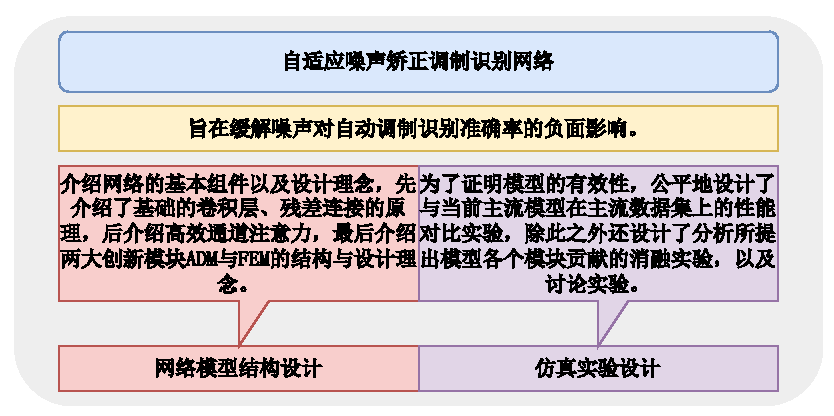
\includegraphics[width=0.9\textwidth]{Image/chap3_map.pdf}
    \caption{本章大纲}
    \label{fig:ad-amr-overview}
\end{figure}

随着通信环境变得日益复杂,自动调制识别(Automatic Modulation Recognition, AMR)系统的性能受到了极大的关注。在实际应用场景中,AMR系统的表现受到诸多环境因素的影响,其中包括噪声、多径效应、多普勒效应等。特别是噪声,由于其不可预测性和变化性,尤其是在现实环境中的强度波动,成为了影响AMR系统性能的主要挑战。

为了应对这一挑战,我们认识到在各种噪声环境下,AMR系统需要具备更强的鲁棒性,以确保其有效性和可靠性。基于此,本研究提出了一种创新的自适应噪声矫正自动调制识别网络(Adaptive Denoising Automatic Modulation Recognition Network, AD-AMR Net),旨在提高系统在不同噪声条件下的调制识别精度和鲁棒性。AD-AMR Net主要由两个核心组成部分构成:自适应噪声矫正模块(Adaptive Denoising Module, ADM)和特征提取模块(Feature Extraction Module, FEM)。在这两个模块中,我们均采用了高效通道注意力模块(Efficient Channel Attention, ECA),以进一步提升网络性能。ADM致力于对噪声分布进行自适应学习,以有效降低输入信号的噪声,从而增强整个AMR系统的鲁棒性。与此同时,特征提取模块利用改进的软阈值化策略,高效提取信号的关键特征,进而提升系统的识别精度。

在实验设计方面,我们精心安排了一系列对比实验,在公开数据集上将AD-AMR Net与近年来的主流模型进行了公平比较。这些实验旨在突出AD-AMR Net在性能方面的优势。此外,为了深入了解网络内各模块的具体作用,我们设计了消融实验。通过这些实验,我们不仅能够评估各个模块对整体性能的贡献,还能探究AD-AMR Net在不同模块组合下的表现。最后,我们还讨论了ADM模块的即插即用特性,即将其集成到其他主流网络中后对性能的提升效果。这些实验结果为评估AD-AMR Net的有效性和灵活性提供了重要依据。



\section{网络模型结构设计}\label{sec:background}

\subsection{卷积层}\label{sec:background}

在深度学习中,卷积层的应用极为广泛,尤其是在图像处理和时间序列数据分析领域。为了全面理解卷积层的工作原理和其强大的功能,本章节将深入探讨卷积层的特点、计算公式以及应用场景。

卷积层通过其独特的参数共享和局部连接机制实现了高效的特征提取。参数共享意味着相同的卷积核在整个输入数据上滑动,从而显著减少了模型的参数数量。而局部连接则确保卷积层能够捕捉到输入数据的局部特征。此外,卷积层由于其设计特性,具有一定程度的平移不变性,使得它能够在不同位置识别相同的特征。卷积层的基本操作可以用以下数学公式表达:
\begin{align}
    \text{Output}(i, j) = \sum_{m}\sum_{n} \text{Kernel}(m, n) \times \text{Input}(i-m, j-n),
    \label{equ: conv}
\end{align}
此公式中,Output表示输出的特征图,Kernel是卷积核,Input是输入的特征图,而m和n代表卷积核在输入上的位置。

\begin{figure}
    \centering
    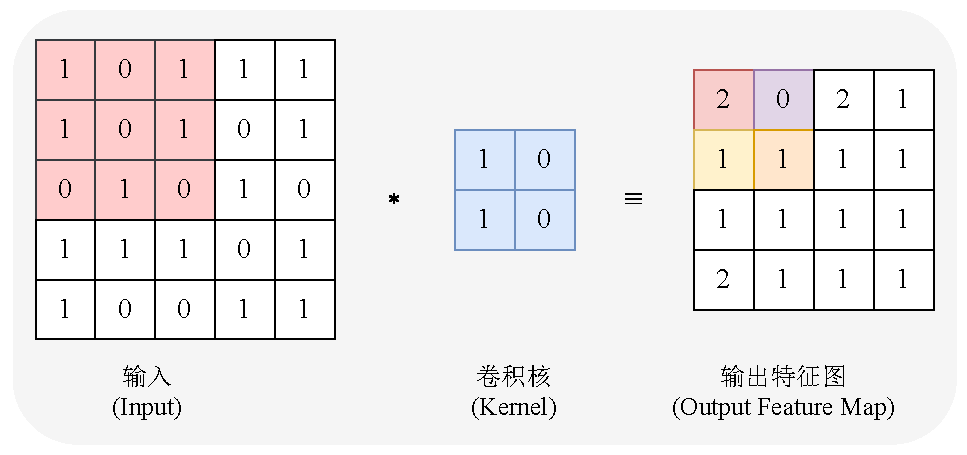
\includegraphics[width=\textwidth]{Image/conv.pdf}
    \caption{卷积操作示意图}
    \label{fig:conv}
\end{figure}

为了更直观地展示卷积操作,图\ref{fig:conv}呈现了一个简化的二维卷积过程。如图所示,输入数据(Input Data)是一个较大的二维网格,卷积核(Convolution Kernel)在其上滑动并执行卷积操作,产生输出特征图(Output Feature Map)。这种视觉表示有助于理解卷积层如何在局部区域应用卷积核来提取特征。


在应用方面,卷积层根据处理数据的维度和特性分为不同的类型。二维卷积(2D Convolution)主要用于处理图像等二维数据,其卷积核在输入图像的高度和宽度两个维度上移动,非常适合提取空间特征。而一维卷积(1D Convolution)则更适用于处理如音频信号或某些金融时间序列这类的一维数据,其卷积核仅沿一个维度(通常是时间轴)移动,有效地捕获序列数据中的时间特征。其数学公式如下:

\begin{align}
    \text{Output}(i) = \sum_{m} \text{Kernel}(m) \times \text{Input}(i-m),
    \label{equ: onedconv}
\end{align}

综上所述,卷积层在现代深度学习架构中扮演着至关重要的角色。它们不仅在图像处理领域展现出强大的能力,也在时间序列数据分析中显示出巨大的潜力,提供了一种强大的方法来提取和分析数据中的关键特征。

\subsection{残差连接}\label{sec:background}

\begin{figure}
    \centering
    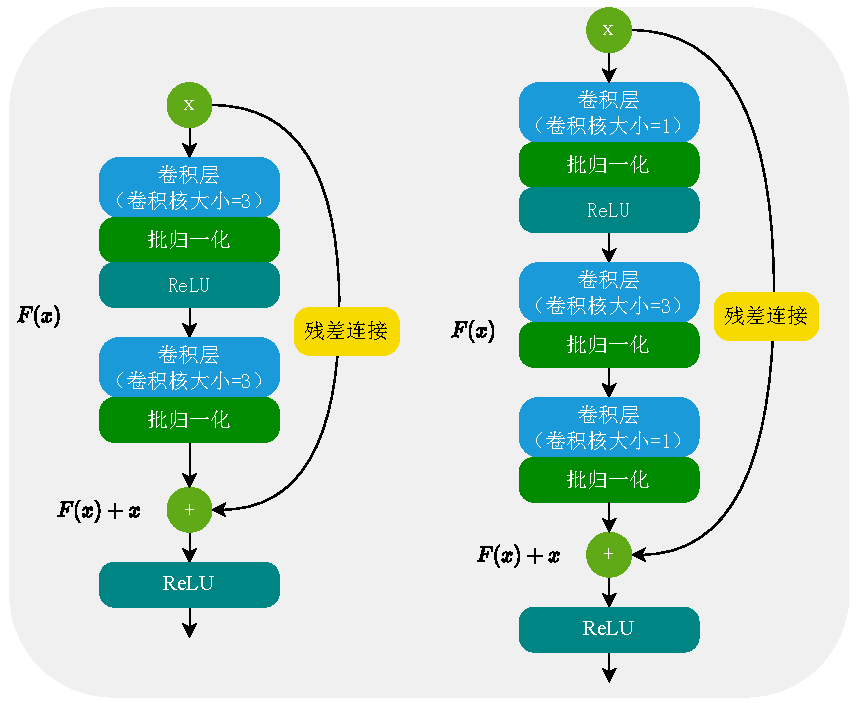
\includegraphics[width=0.8\textwidth]{Image/residualblock_cn.pdf}
    \caption{残差连接示意图,其中左边为普通残差块,右边为瓶颈残差块}
    \label{fig:residual}
\end{figure}

在深度学习的发展过程中,随着神经网络结构变得越来越深,网络的训练变得日益困难。这主要是因为在深层网络中常见的梯度消失和梯度爆炸问题,这些问题严重影响了网络性能的提升和模型的训练效率。为了克服这些挑战,残差连接(Residual Connection)的概念被引入到深度神经网络的设计中\cite{he2016deep},特别是在复杂的图像处理任务中。本章节旨在探讨残差连接的原理、其带来的实际效果,以及在实际应用中的重要性。

残差连接的核心思想是通过添加一种直接的路径,将输入信息直接传递到网络的后续层,从而解决深层网络中的信息流失问题。数学上,这可以表示为:

% \[ \text{Output} = \text{Activation}(\text{Conv}(X) + X) \]
\begin{align}
    \text{Output} = \text{Activation}(\text{Conv}(X) + X),
    \label{equ: residual}
\end{align}

在这个公式中,X代表输入特征图,Conv代表卷积层操作,Activation是激活函数,Output是残差块的输出。残差连接通过加法操作将输入直接与卷积层的输出相加,这种设计使得网络可以学习到输入与输出之间的残差,即输出与输入的差异。

残差连接的引入为深度学习带来了革命性的影响。在ResNet(Residual Network)等基于残差连接的架构中,网络能够通过残差连接维持较深层次时信息的流动性和有效性,从而避免了梯度消失的问题。实际效果中,ResNet架构在各种图像识别竞赛中取得了显著的成绩,比如在ImageNet挑战中大幅提升了分类精度,显示出强大的学习能力和泛化性能。

此外,残差连接的设计也促进了深层网络训练的稳定性。由于残差连接的存在,深层网络中的梯度能够有效地传递,大大减少了训练深层网络时的困难。这种优势使得研究人员能够构建更深层次的网络,探索更复杂的模型结构,从而在诸如图像分类、物体检测和语义分割等任务中取得更好的性能。

综合来看,残差连接不仅解决了深层网络训练中的关键难题,还推动了深度学习在诸多领域的广泛应用和快速发展。通过提供一种有效的信息传递机制,残差连接改善了深层神经网络的训练效果和模型性能,被视为现代深度学习架构设计中的一个重要里程碑。

% \subsection{高效通道注意力}\label{sec:background}
% \begin{figure}
%     \centering
%     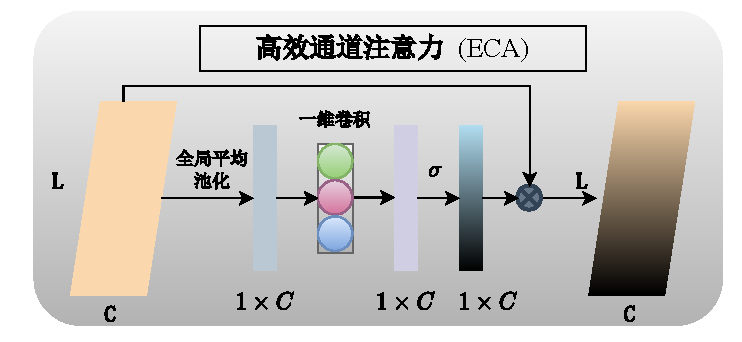
\includegraphics[width=0.6\textwidth]{Image/eca.jpg}
%     \caption{高效通道注意力模块}
%     \label{fig:eca}
% \end{figure}

% 通道注意机制(Channel Attention Mechanism, CAM)在当前的卷积神经网络中被广泛应用于各种任务。其中,挤压激励模块(Squeeze and Excitation Module, SEM)是一种备受欢迎的通道注意机制,它通过挤压和激励操作来捕捉通道之间的依赖关系。然而,SEM的一个局限性在于它依赖于计算开销较大的全连接层,用于学习注意力权重。尤其在输出通道较大的情况下,SEM可能导致显著的计算成本,同时还会增加网络的内存占用,限制了其在资源受限环境中的应用。

% 为了解决这一问题,我们引入了ECA模块,这是一种轻量但高效的通道注意机制,专门设计用于实现高泛化能力。如图~\ref{fig:eca}所示,ECA模块由全局平均池化(Global Average Pooling, GAP)层、一维卷积层和sigmoid激活组成,因此需要的参数远远少于SEM。具体而言,GAP层将特征图总结成一个全局上下文向量,以捕捉跨通道的依赖关系。这种全局池化的思想受益于自然图像中的平移不变性,有助于捕捉特征的整体信息。

% 接着,一维卷积层将这个全局上下文向量转换为通道注意权重。相较于全连接层,卷积层具有参数共享和局部感受野的优势,使得ECA模块能够更加灵活地捕捉通道间的关系。通过sigmoid函数将注意权重缩放到0到1之间,sigmoid函数的定义如下:
% %sigmoid函数
% \begin{equation}
% \begin{aligned}
% \text{sigmoid}(x) = \frac{1}{1 + \text{exp}(-x)}.
% \end{aligned}
% \label{equ: sigmoid}
% \end{equation}

% 通过与输入特征进行逐元素乘法,ECA模块突出显示信息丰富的特征并抑制不太相关的特征。这种非线性的特征放大和抑制机制有助于提高模型对关键信息的关注度,从而提升性能。尽管ECA模块的设计相对简单,但经验结果表明,与SEM相比,它在使用更少的参数和计算资源的情况下能够实现更好的性能。这使得ECA模块成为计算通道注意力的一种高效且轻量级的选择。在实际应用中,ECA模块在图像分类、目标检测等任务中展现了出色的通用性和性能。

\subsection{高效通道注意力}\label{sec:background}
\begin{figure}
\centering
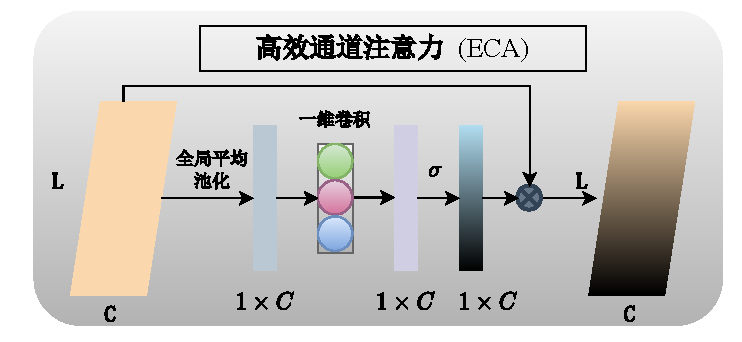
\includegraphics[width=0.8\textwidth]{Image/eca.pdf}
\caption{高效通道注意力模块}
\label{fig:eca}
\end{figure}

通道注意机制(Channel Attention Mechanism, CAM)已在现代卷积神经网络中被广泛应用于多种任务,以提升其性能。特别地\cite{wang2020eca},挤压激励模块(Squeeze and Excitation Module, SEM)是一种流行的CAM实现,它通过挤压和激励操作来有效捕获通道间的相关性。然而,挤压激励模块在学习注意力权重时依赖于计算成本较高的全连接层,特别是当输出通道数量较大时,可能带来显著的计算和内存开销,从而限制了其在资源有限的环境下的应用。

为应对这一挑战,我们引入了一种轻量级且高效的通道注意机制——高效通道注意力(ECA)模块。如图~\ref{fig:eca}所示,ECA模块是一种在现代卷积神经网络中应用的通道注意机制,它基于挤压和激励(squeeze-and-excitation, SE)模块的设计理念,但在减少模型复杂度方面做了改进,尤其是避免了维度降低的问题。ECA模块通过不进行通道维度的降低,能够更直接地捕捉不同通道间的关系,从而提高了注意力学习的效率。

具体来说,ECA模块首先利用全局平均池化(Global Average Pooling, GAP)操作来聚合特征,然后通过一维卷积来获取每个通道及其邻近通道的交互信息。这样的设计使得ECA模块可以更高效地实现局部跨通道的交互。此外,一维卷积的核大小(kernel size)决定了局部跨通道交互的覆盖范围,即决定了在注意力预测中有多少相邻通道参与。ECA模块的这种设计不仅降低了参数数量,而且提高了计算效率,使得它在大规模图像分类、目标检测等任务中表现出色。相较于传统的SE模块,ECA模块在资源受限的环境下具有更好的应用潜力。

在经过上述的运算之后ECA会得到一个$1 \times C$的权重向量,经过sigmoid函数处理,这些权重被缩放到0至1的范围内。sigmoid函数定义如下:
%sigmoid函数
\begin{equation}
\begin{aligned}
\text{sigmoid}(x) = \frac{1}{1 + \text{exp}(-x)}.
\end{aligned}
\label{equ: sigmoid}
\end{equation}

ECA模块通过与输入特征进行逐元素乘法操作,有效地突出显示重要特征并抑制不太相关的特征。这种非线性的特征增强和抑制机制显著提升了模型对关键信息的敏感度,进而提高整体性能。值得注意的是,尽管ECA模块的设计相对简单,但它在实际应用中——如图像分类、目标检测等任务——表现出了优异的通用性和性能,同时在参数和计算资源方面的经济性使其成为处理通道注意力的高效且轻量级的选择。

% \subsection{自适应噪声矫正模块具体设计}\label{sec:background}

% \begin{figure}
%     \centering
%     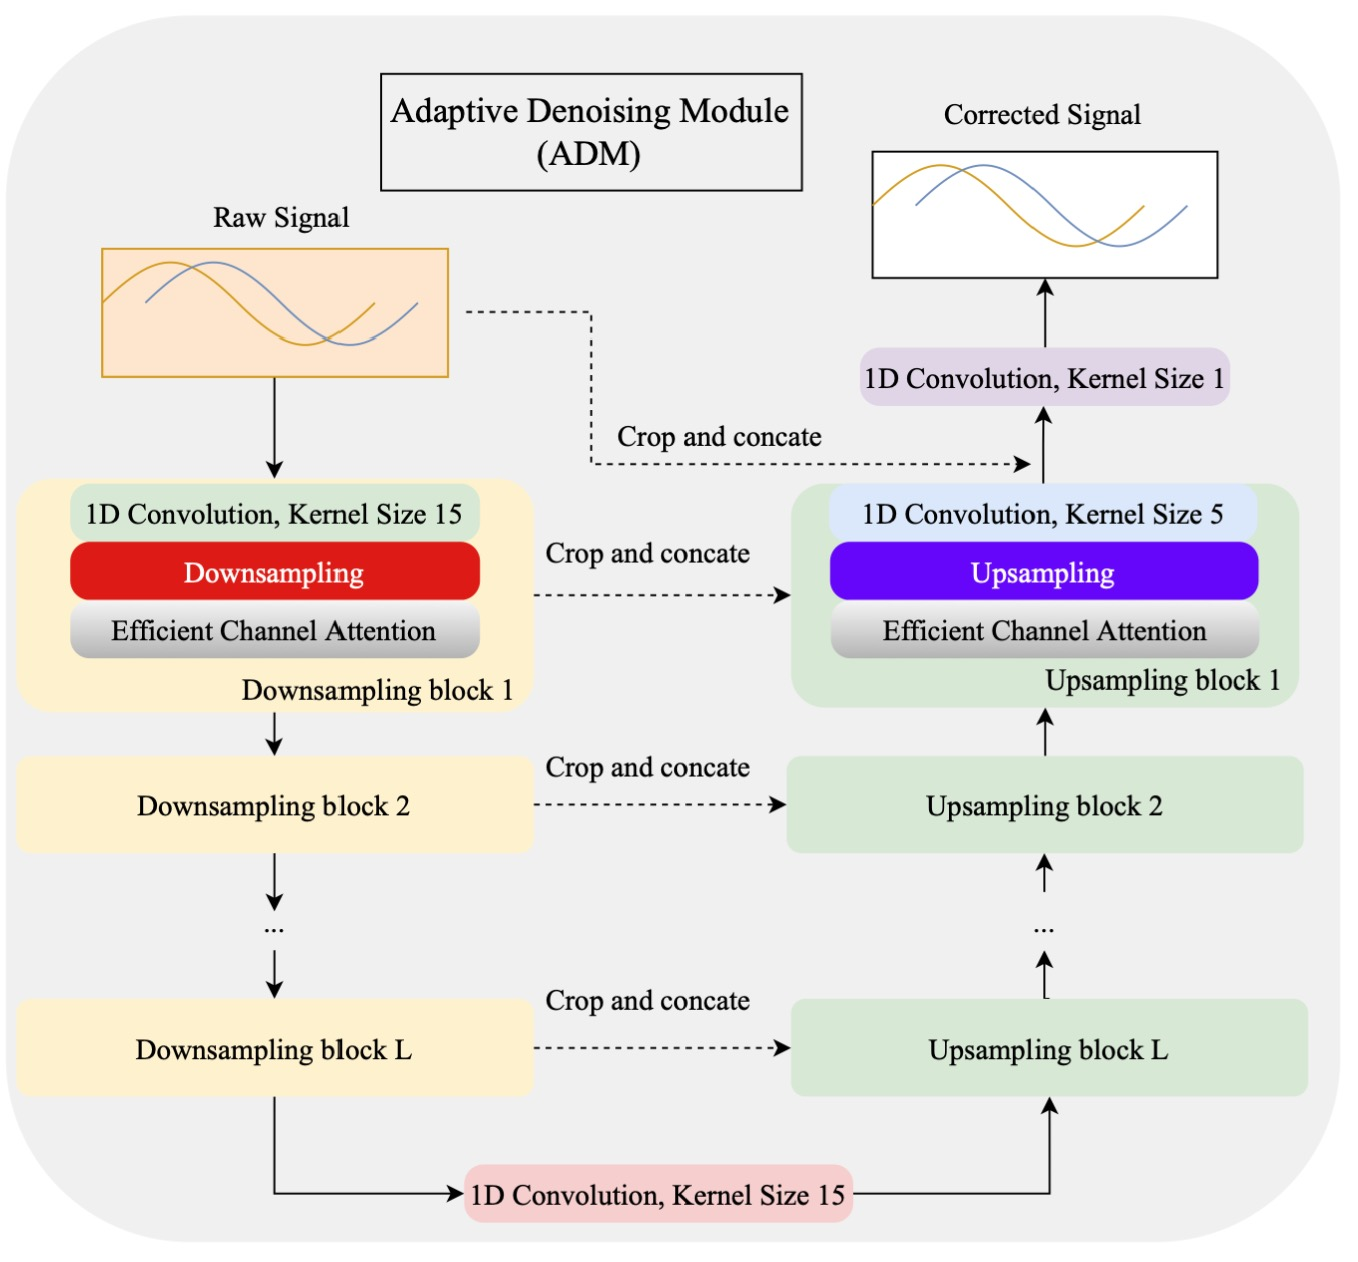
\includegraphics[width=0.6\textwidth]{Image/adm.jpg}
%     \caption{自适应降噪模块}
%     \label{fig:adm}
% \end{figure}

% 复杂信号作为一种时间序列数据,往往受到各种噪音和偏移的影响。在这种背景下,我们通过将ECA集成到WaveUNet架构中,提出了一种称为ADM(Adaptive Denoising Module)的解决方案,旨在有效减轻这些干扰的影响。ADM的设计灵感源自ECA和WaveUNet,结合了通道注意机制和波形处理网络的优势。

% ADM的核心目标是接收带有噪音的输入信号,并通过学习抑制噪音,同时保留信号的真实基础结构,从而生成一个去噪版本的输出。通过在网络的训练过程中,ADM部分成功地拟合了原始信号,使得输出信号更加清晰,噪音水平相应降低。这一观察结果得到了在文献中的验证~\cite{michelashvili2019speech}。

% ADM的架构如图~\ref{fig:adm}所示,包含了一系列下采样和上采样块。在这些块中,每个都包括一个1D卷积层(卷积核大小为15)用于学习局部特征,一个下采样或上采样操作以处理不同尺度的信息,以及一个ECA模块来强调具有信息量的特征。下采样的目的是在更广泛的上下文中整合信息,以及通过减少分辨率来关注大尺度信号组成部分,而上采样则恢复分辨率,并允许模型整合来自更粗糙尺度编码的信息。

% 关键的设计特点之一是通过裁剪和连接的跳跃连接,实现了编码信息在不同尺度之间的传递。这样的设计保留了本地和全局上下文,有助于捕捉信号的复杂结构。最终,通过一个1D卷积层(卷积核大小为1)在通道上整合,生成去噪输出。这个层级处理和聚合信息的过程使得ADM能够分离有意义的信号成分并抑制噪音,从而在实际应用中取得显著效果。

% 通过将嘈杂信号输入到ADM中,我们能够从中解开清晰信号的组成部分,从而在复杂信号处理中提供了一种有效的工具。这种整合了通道注意机制的ADM设计不仅在噪音抑制上取得了令人满意的效果,而且在保留信号关键特征的同时,减少了计算复杂度,使得其成为时间序列数据处理中的一种有前景的方法。

\subsection{自适应噪声矫正模块具体设计}\label{sec:background}

\begin{figure}
\centering
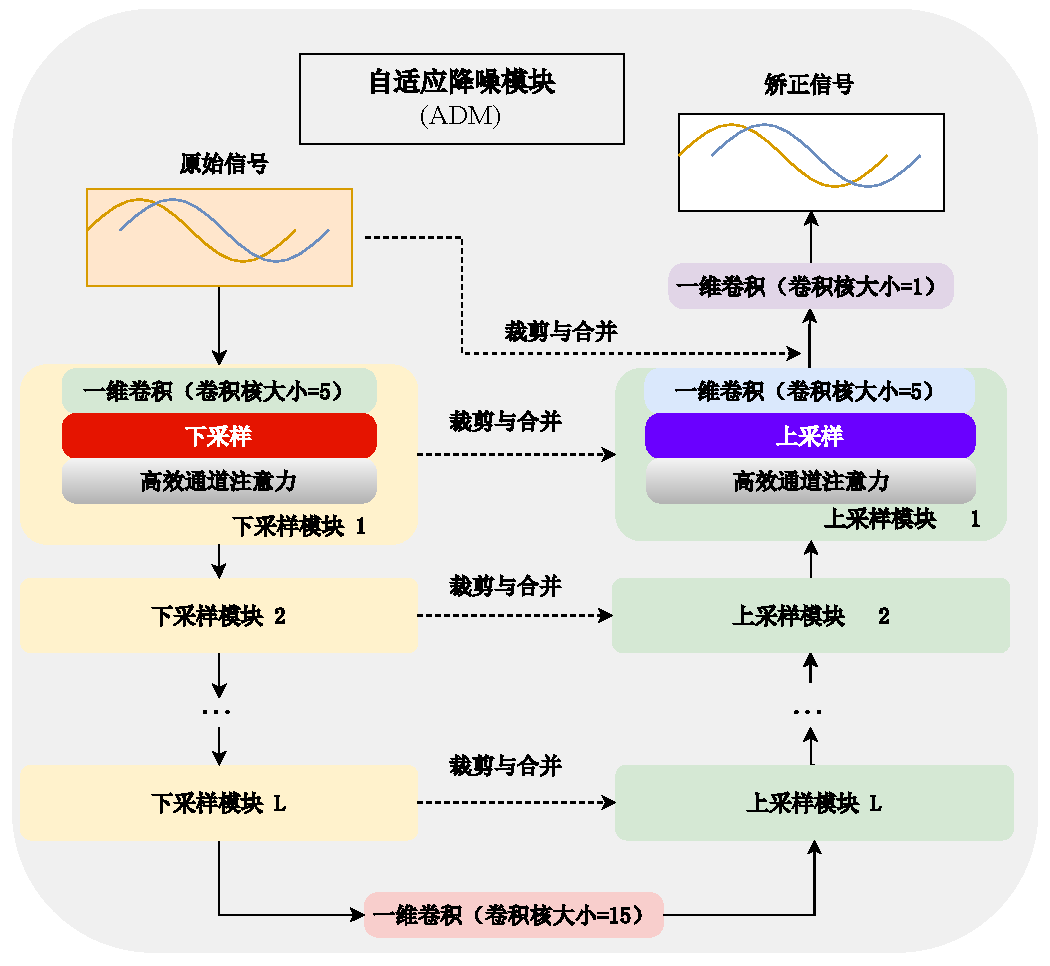
\includegraphics[width=0.8\textwidth]{Image/adm.pdf}
\caption{自适应降噪模块}
\label{fig:adm}
\end{figure}

在处理复杂的时间序列信号时,经常面临多种噪声和干扰的挑战。针对这一问题,我们结合了高效通道注意力(ECA)模块和WaveUNet架构的特性,设计了ADM(Adaptive Denoising Module)。ADM不仅从ECA中借鉴了通道注意机制的优势,还引入了WaveUNet在处理音频信号方面的深层次多尺度特征提取能力。

ADM的主要任务是接收带有噪声的输入信号,并通过先进的学习机制有效地降低噪声,同时保留信号的原始结构。其核心是利用WaveUNet的多层次结构来进行深入的信号分析。在训练过程中,ADM能够对原始信号进行高度拟合,从而在输出端提供更加清晰、噪声水平更低的信号。这一成果已得到相关研究的支持和验证~\cite{michelashvili2019speech}。

ADM的架构如图~\ref{fig:adm}所示,它包含了一系列的下采样和上采样块,类似于WaveUNet的设计。这些块中每个都包含一个1D卷积层(卷积核大小为15),用以学习局部特征,一个下采样或上采样操作处理不同尺度的信息,以及一个ECA模块以突出重要特征。下采样的目的是在更广泛的上下文中整合信息,并关注大尺度信号组成部分,而上采样则用于恢复分辨率,整合更粗糙尺度编码的信息。

特别地,ADM的一个关键设计特点是通过裁剪和连接实现的跳跃连接。这些连接在不同尺度之间传递编码信息,保留了局部和全局上下文,有助于捕捉信号的复杂结构。最终,一个1D卷积层(卷积核大小为1)在通道上进行整合,生成清晰的去噪输出。这种层级化的信息处理和聚合方式使得ADM不仅能够有效分离有意义的信号成分并抑制噪声,还能够在不增加过多计算负担的情况下,实现对信号细节的精确还原。

将含有噪声的信号输入ADM后,我们可以有效地提取出清晰的信号成分,尤其是在复杂的信号处理任务中,如音频信号分离、语音增强等应用场景。这种结合了通道注意力机制和多层次信号处理能力的ADM设计,不仅在噪声抑制方面表现出色,还在保持信号关键特征的同时优化了计算效率,展现出在复杂时间序列数据处理中的巨大潜力。

% \section{特征提取模块}\label{sec:background}

% \begin{figure}
%     \centering
%     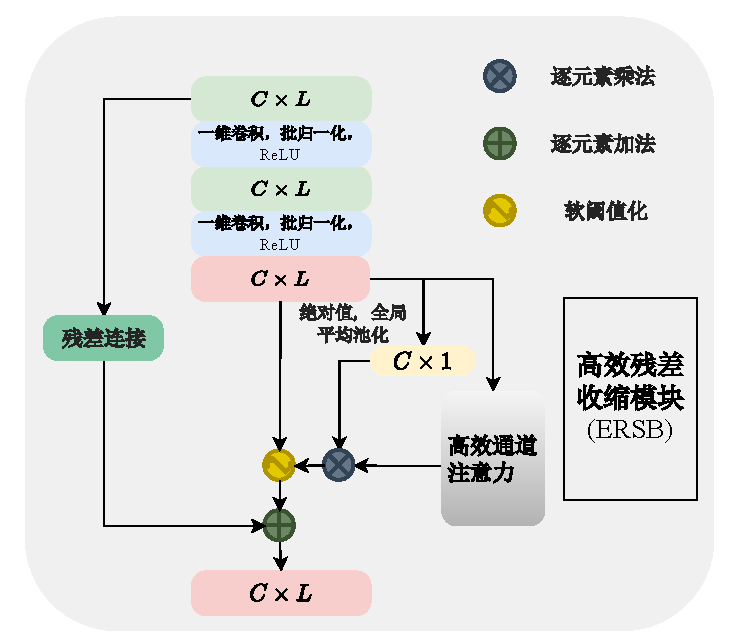
\includegraphics[width=0.6\textwidth]{Image/fem.jpg}
%     \caption{多尺度特征提取模块}
%     \label{fig:fem}
% \end{figure}

% \begin{equation}
%     \begin{aligned}
%             \text{soft-threshold}(x, \lambda) = \begin{cases}
%             x - \lambda, & x > \lambda \\
%             0, & -\lambda \leq x \leq \lambda \\
%             x + \lambda, & x < -\lambda,
%             \end{cases}
%         \end{aligned}
%     \label{equ: soft}
% \end{equation}

% FEM(Feature Extraction Module)的设计旨在从去噪信号中抽取具有多尺度特征的有力表示。采用层次化结构,FEM集成了多个ERSB(Enhanced Residual Shrinkage Block),这种设计灵感源自ResNet架构。ERSB的构建是基于Deep Residual Shrinkage Network中RSB(Residual Shrinkage Block)的思想~\cite{zhao2019deep},但在这里,我们采用了更为高效的ECA模块替代了原始的SE块。如图~\ref{fig:fem} 的右上角所示,ERSB由两个卷积层、身份快捷方式、自适应软阈值操作和ECA模块组成。

% 身份快捷方式的引入不仅使得训练过程中信息流畅通,而且有助于在网络层次中实现梯度的良好传播。自适应软阈值操作,如式~\eqref{equ: soft} 所示,是一种在信号处理领域广泛应用的方法,通过将微小的值置零来实现噪音抑制。ERSB内的自适应软阈值操作与传统的手工设计滤波器不同,它经过训练以自动确定阈值,从而更加适应多样的信号特征。此外,ECA模块通过跨通道整合信息,以更少的参数实现对特征的细致优化,并在泛化性能上胜过SE模块。

% 通过堆叠具有身份快捷方式的多个ERSB,FEM能够分层提取输入信号的多尺度表示,灵活地适应信号的不同频率和结构。这种层次化的特征提取使得FEM能够自适应地将不相关的特征抑制,从而得到更具信息含量的表示。综合来看,身份快捷方式、软阈值操作和ECA模块相互协作,使得FEM在处理输入信号时能够稳健地提取出干净而丰富的多尺度特征。在FEM的详细配置中,我们采用了1D卷积层作为主干,并通过减少输出通道数目来适应信号分类任务,以此平衡了性能和计算复杂性。

\subsection{特征提取模块}\label{sec:background}

\begin{equation}
    \begin{aligned}
            \text{soft-threshold}(x, \lambda) = \begin{cases}
            x - \lambda, & x > \lambda \\
            0, & -\lambda \leq x \leq \lambda \\
            x + \lambda, & x < -\lambda,
            \end{cases}
        \end{aligned}
    \label{equ: soft}
\end{equation}

\begin{figure}
\centering
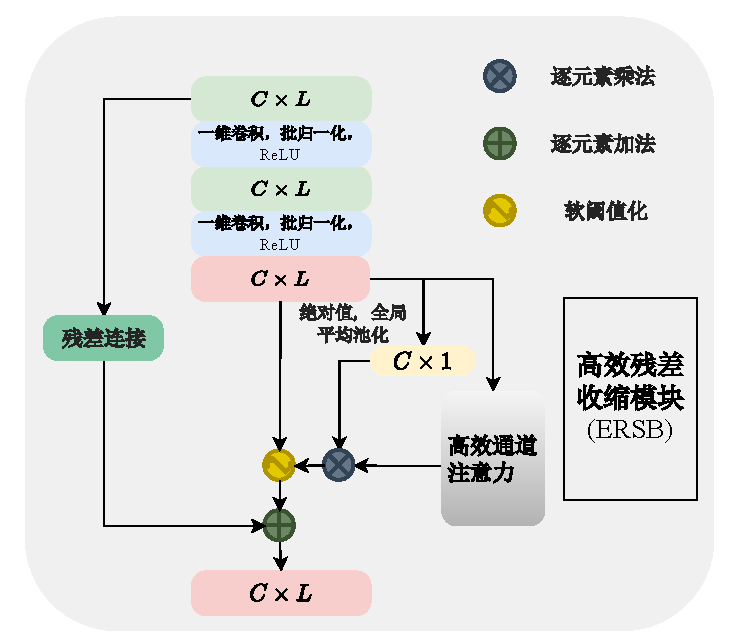
\includegraphics[width=0.8\textwidth]{Image/fem.pdf}
\caption{高效残差收缩模块}
\label{fig:fem}
\end{figure}

FEM(Feature Extraction Module)的设计核心在于从经过降噪处理的信号中有效地提取出具有丰富多尺度特征的表示。本模块采用分层化结构,并集成了多个增强残差收缩块(Enhanced Residual Shrinkage Block, ERSB),这一设计受到了深度残差网络(ResNet)架构的启发。ERSB的构建基于深度残差收缩网络中的残差收缩块(Residual Shrinkage Block, RSB)的概念~\cite{zhao2019deep}。然而,在FEM中,我们采用更高效的ECA模块来替换原始的SE块,以提升网络的性能和效率。

ERSB的设计包括两个关键部分:卷积层和残差连接。卷积层用于捕获信号的局部特征,而残差连接则保证信息的流畅传递,并有助于实现网络层次中梯度的有效传播。此外,我们还引入了自适应软阈值操作,如式~\eqref{equ: soft}所示。这种操作在信号处理领域被广泛应用,用于抑制微小的信号值,从而降低噪音的影响。不同于传统的手动阈值设置,ERSB内的软阈值操作通过训练自动调整,更好地适应多样化的信号特征。

ECA模块在ERSB中发挥着至关重要的作用,它通过跨通道信息整合来精细调节特征,使用较少的参数便达到了优越的泛化能力,超越了SE模块的性能。

FEM通过堆叠多个具有残差连接的ERSB,实现了对输入信号的多层次、多尺度特征提取。这种分层提取机制赋予FEM能够灵活应对信号的各种频率和结构变化。层次化的特征提取方法使得FEM能够有效地抑制不相关特征,提取出更加丰富和信息密集的特征表示。通过这样的结构设计,残差连接、软阈值操作和ECA模块相互协作,确保了FEM在处理输入信号时的稳定性和有效性。

在FEM的具体配置中,我们主要采用1D卷积层作为其主要结构,同时通过调整输出通道数目来适应不同的信号分类任务,实现了性能与计算复杂性之间的平衡。

\begin{figure}
    \centering
    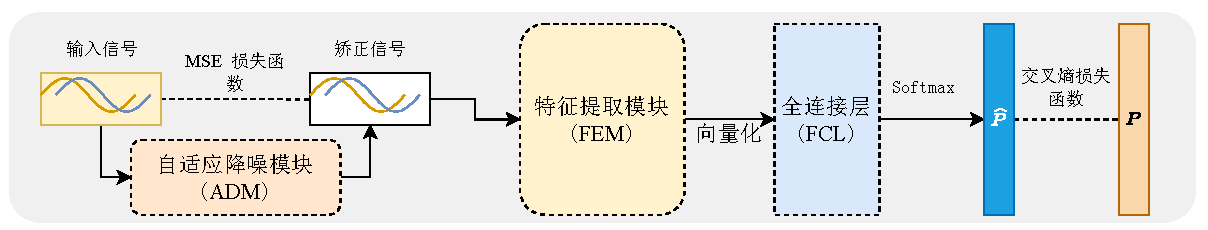
\includegraphics[width=\textwidth]{Image/ad-amr-overview_cn.pdf}
    \caption{整体框架图}
   \label{fig:ad-amr-overview}
\end{figure}

\section{仿真结果}\label{sec:background}
% 数据集 RadioML 2016.10A、 RadioML 2016.10B 和 RadioML 2018.01A
% 以 6:2:2 的比例划分为训练集、验证集和测试集
% 平台:PyTorch 框架,NVIDIA RTX 3090 GPU
% Adam 优化器,学习率为 0.001
% 100 个 epochs, early stopping 技术
% reduce learning rate on plateau 技术用于自适应地调整学习率以搜索最佳参数
% OA、宏平均 F1 分数、Kappa 系数和参数数量作为评价指标
% 比较试验:RadiML 2016.01A 数据集: CNN CLDNN SVM AMC-Net
% 比较试验:RadiML 2016.01B 数据集: CNN CLDNN ResNet AMC-Net
% 比较试验:RadiML 2018.01A 数据集: CNN CLDNN ResNet SENet AWN
% 消融实验: 去掉 ECA 模块 、 去掉 ADM 模块 、 两者都去掉 (同时在上述三个数据集上进行)
% 讨论实验:在现有的模型上添加 ADM 模块,比较结果 (在上述三个数据集上进行)
% 评估指标:OA、宏平均 F1 分数、Kappa 系数和参数数量
\subsection{实验设置}

% #### 数据集及划分
在本研究中,我们旨在评估自适应噪声矫正调制识别网络(ADM)的性能,并与现有的方法进行比较。实验使用了RadioML 2016.10A、RadioML 2016.10B 和 RadioML 2018.01A三个数据集,输入尺寸分别为$2 \times 128$, $2 \times 128$和$2 \times 1024$,它们包含了不同类型的调制信号,适用于评估调制识别算法的性能。数据集被分为训练集、验证集和测试集,按照6:2:2的比例划分。这种划分旨在确保模型在各种条件下都能进行充分的训练和公正的评估。

% #### 实验平台
实验在PyTorch框架下进行,利用NVIDIA RTX 3090 GPU进行计算。PyTorch是当前深度学习研究中广泛使用的框架之一,其灵活性和强大的计算能力为本实验提供了支持。模型的训练采用Adam优化器,初始学习率设置为0.001。所使用的损失函数为交叉熵损失函数,用于衡量模型输出与真实标签之间的差异。交叉熵损失函数的定义如下:

% 交叉熵损失函数
\begin{equation}
\begin{aligned}
\text{CrossEntropy}(y, \hat{y}) = -\sum_{i=1}^{N} y_i \log(\hat{y}_i),
\end{aligned}
\label{equ: crossentropy}
\end{equation}
其中$y$表示真实标签,$\hat{y}$表示模型输出,$N$表示类别数量。

整个训练过程包括100个epochs(训练周期),同时采用了早停止 (early stopping)技术以防止过拟合。早停止是一种在机器学习和深度学习中常用的技术,用于防止模型过拟合同时提高训练效率。这种技术的核心在于监控模型在一个独立的验证集上的性能。在训练过程中,除了在训练集上学习,模型还会在这个验证集上进行评估。验证集通常包含未用于训练的数据,它模拟了模型在未知数据上的表现。早停止的关键在于设置一个“耐心”参数,它定义了在性能没有显著提升的情况下模型继续训练的epoch数量。如果在这些epoch内,模型在验证集上的性能没有提升,或者性能开始下降,训练过程将提前终止。这样做的目的是防止模型过度学习训练数据的特定特征,即防止过拟合,确保模型在未知数据上具有更好的泛化能力。同时,早停止还可以避免在训练深层和复杂网络时的不必要计算,节约计算资源。由于其简单性和有效性,早停止已成为训练深度学习模型时的一个重要工具,尤其在处理大型数据集或构建复杂模型时尤为重要。此外,为了在训练过程中自适应地调整学习率,我们采用了平台期衰减学习率 (reduce learning rate on plateau)技术,平台期衰减学习率 是一种在深度学习训练中常用的学习率调整策略,旨在改善模型在训练过程中的性能和收敛速度。这种方法特别适用于处理模型训练过程中遇到的性能停滞或提升缓慢的情况。当使用这种策略时,学习率的调整基于模型在验证集上的性能指标,如损失或准确率。在连续若干个epoch中,如果模型的性能没有显著提升,即进入了平台),学习率将被自动减少。具体来说,如果模型在设定的epoch数量内未能达到预定的性能改善阈值,学习率会乘以一个事先定义的因子(通常小于1)进行减小。例如,如果当前学习率是0.001,乘以一个因子0.1后,新的学习率将变为0.0001。这种方法的主要优点是在训练过程中提供了一种自适应机制,有助于细致地调整学习率,从而克服学习停滞的挑战。通过降低学习率,模型在参数空间中的搜索步长减小,这有助于更精细地探索,并有可能找到更优的局部最优解。平台期衰减学习率 策略在训练深度网络、尤其是在复杂或高度非凸优化问题中非常有效。它可以避免模型在训练早期由于较大学习率导致的过快收敛到非最优解,同时在训练后期通过更小的学习率细致调整,以提升模型性能。此外,这种策略还有助于提高模型训练的稳定性和可靠性,尤其是在处理大规模数据集时。

% ### 评价指标
我们选用了准确率(Overall Accuracy, OA)、宏平均F1分数、Kappa系数和模型参数数量作为评价指标。OA提供了整体性能的概览,宏平均F1分数评估了模型在不同类别上的均衡性能,Kappa系数则衡量了分类准确性相对于随机分类的改善。参数数量反映了模型的复杂度。
OA定义为:
\begin{equation}
        \begin{aligned}
            \text{OA} = \frac{\sum_{i=1}^{M}TP_i}{\sum_{i=1}^{M}TP_i + \sum_{i=1}^{M}FP_i},
        \end{aligned}
    \label{equ: oa}
\end{equation}
F1分数定义为:
\begin{equation}
    \begin{aligned}
        \text{F1-score} = \frac{2\sum_{i=1}^{M}TP_i}{2\sum_{i=1}^{M}TP_i + \sum_{i=1}^{M}FP_i + \sum_{i=1}^{M}FN_i},
    \end{aligned}
    \label{equ: f1}
\end{equation}
Kappa系数定义为:
\begin{equation}
    \begin{aligned}
        \text{Kappa} = \frac{\text{OA} - \mathbb{P}(\text{Chance})}{1 - \mathbb{P}(\text{Chance})},
    \end{aligned}
    \label{equ: kappa}
\end{equation}
其中$TP_i$是正确分类为第$i$种调制的样本数量,$FP_i$是错误分类为第$i$种调制的样本数量,$\mathbb{P}(\text{Chance})$表示随机分类的概率。

% ### 比较试验
为了全面评估ADM的性能,我们在三个数据集上进行了一系列比较试验,具体的实验内容如表~\ref{tab:experiment_summary}所示。

\begin{table}[htpb]
    \centering
    \caption{实验概览}
    \resizebox{\textwidth}{!}{%
    \label{tab:experiment_summary}
    \begin{tabular}{cm{0.25\textwidth}m{0.25\textwidth}m{0.5\textwidth}}
    \hline
    \textbf{实验类型} & \textbf{RadiML 2016.10A} & \textbf{RadiML 2016.10B} & \textbf{RadiML 2018.01A} \\ \hline
    基准比较 & CNN, CLDNN, SVM & ResNet, AMC-Net & CNN, CLDNN, ResNet, SENet, AWN \\ \hline
    消融实验 & \multicolumn{3}{c}{1. 去掉ECA模块, 2. 去掉ADM模块, 3. 将前两者都去掉} \\ \hline
    讨论实验 & \multicolumn{3}{c}{在现有模型(CNN, CLDNN, ResNet, SENet, AWN) 上添加ADM模块} \\ \hline
    \end{tabular}
    }
\end{table}

在本研究中,我们精心设计了一系列实验,以全面评估自适应噪声矫正调制识别网络(ADM)的性能,并将其与当前的主流方法进行比较。实验设计的理念是基于不同数据集的特性来选择最合适的比较模型,以确保评估的全面性和公正性。

首先,我们选择了RadioML 2016.10A数据集进行初步的性能比较。这个数据集相对较小,因此特别适合用来评估简单模型的性能,并与传统的算法,如支持向量机(SVM),进行比较。由于数据集的规模较小,它提供了一个理想的环境,用于快速验证模型的基本性能和稳定性。在这个阶段,我们主要关注模型在基本调制识别任务上的能力,以及它与传统机器学习方法在处理这类问题时的相对优势。

随后,我们转向RadioML 2016.10B数据集,该数据集在样本维度上与2016.10A一致,但总体规模更大。较大的数据集规模使得它更适合用来评估近几年深度学习模型的性能。在这个阶段,我们将AD-AMR Net与如残差网络(ResNet),AMC-Net等近年来流行的深度学习模型进行对比。通过这样的比较,我们能够更好地理解ADM在处理相对复杂的数据集时的表现,以及其在现代深度学习框架中的竞争力。

最后,我们使用RadioML 2018.01A数据集,这是一个在样本维度和数据集本身都较大的数据集。这个数据集适合用来与当前主流的深度学习模型进行比较,如SENet和自适应小波网络(AWN)。这个阶段的实验不仅能够展示AD-AMR Net在处理大规模、高维度数据时的能力,还能揭示其在最先进的模型面前的性能和适应性。

在消融实验中,我们的主要目的是证明所提出模块的有效性。通过分别去掉ECA模块、ADM模块以及两者都去掉的设置,我们可以详细分析每个组件对整体性能的贡献,以及它们之间的相互作用。这种方法能够清晰地展示每个模块的重要性,以及它们如何共同作用以提高模型的整体性能。消融实验的具体设置如下:
\begin{enumerate}
    \item AD-AMR Net:完整的提出模型。

    \item AD-AMR~-~1:去除ADM的提出模型。

    \item AD-AMR~-~2:去除FEM中ERSB的提出模型。

    \item AD-AMR~-~3:去除ADM和FEM中ERSB的提出模型。
\end{enumerate}

此外,在讨论实验中,我们探讨了ADM模块的“即插即用”能力,即评估将ADM模块加入到现有模型中时的效果。这项工作不仅验证了ADM模块的通用性,还展示了其在不同架构中的适应性和效果。通过这些实验,我们能够全面评价ADM模块在不同设置和环境下的实际应用价值。讨论实验的具体设置如下:
\begin{enumerate}
    \item ADM-CNN:带有ADM的CNN。
    \item ADM-CLDNN:带有ADM的CLDNN。
    \item ADM-AWN:带有ADM的AWN。
\end{enumerate}

综上所述,通过这些精心设计的实验,我们不仅能够全面评估ADM在不同数据集和环境中的性能,还能深入理解其与现有方法的比较情况,以及单独模块对整体性能的影响。这些实验结果将为调制识别领域的研究提供宝贵的见解,推动相关技术的进一步发展。

% 我们在PyTorch中实现了AD-AMR Net,并在NVIDIA RTX 3090 GPU上从头开始进行了训练。网络经过了100个epochs的训练,使用了Adam优化器,学习率为0.001。我们采用了\textit{early stopping}技术,即如果验证损失在连续10次迭代后不再减小,则停止训练,以防止过拟合并提高训练效率。

% 为了自适应地调整学习率以搜索最佳参数,我们还采用了\textit{reduce learning rate on plateau}技术,即当损失指标停止改善时减小学习率。这种自适应调整有助于更有效地在参数空间中导航。

% 对于训练和评估,我们选择了RadioML 2018.01A数据集~\cite{o2018over}。该数据集提供了一个全面的场景集,可以在不同的无线信道效应下对AD-AMR Net进行深入检查,包括多径衰落、采样率偏移、加性白噪声(AWGN)和中心频率偏移等。

% 在整个训练和评估阶段,我们进行了数值分析,以评估所提出方案的性能。通过在不同无线信道条件下进行测试,验证了模型的鲁棒性和适应性。这次全面的评估旨在展示AD-AMR Net在处理不同信道干扰引起的真实世界挑战方面的有效性。

% \subsection{性能指标}

% 我们使用整体准确度(Overall Accuracy, OA)、宏平均F1分数、Kappa系数和参数数量作为评价指标,其中
% OA定义为:
% \begin{equation}
%         \begin{aligned}
%             \text{OA} = \frac{\sum_{i=1}^{M}TP_i}{\sum_{i=1}^{M}TP_i + \sum_{i=1}^{M}FP_i},
%         \end{aligned}
%     \label{equ: oa}
% \end{equation}
% F1分数定义为:
% \begin{equation}
%     \begin{aligned}
%         \text{F1-score} = \frac{2\sum_{i=1}^{M}TP_i}{2\sum_{i=1}^{M}TP_i + \sum_{i=1}^{M}FP_i + \sum_{i=1}^{M}FN_i},
%     \end{aligned}
%     \label{equ: f1}
% \end{equation}
% Kappa系数定义为:
% \begin{equation}
%     \begin{aligned}
%         \text{Kappa} = \frac{\text{OA} - \mathbb{P}(\text{Chance})}{1 - \mathbb{P}(\text{Chance})},
%     \end{aligned}
%     \label{equ: kappa}
% \end{equation}
% 其中$TP_i$是正确分类为第$i$种调制的样本数量,$FP_i$是错误分类为第$i$种调制的样本数量,$\mathbb{P}(\text{Chance})$表示随机分类的概率。

% \dots

% \subsection{基准比较}
% 为了评估,将使用以下方法与所提出的方案进行比较作为基准:
% \begin{enumerate}
%     \item \textit{CNN}~\cite{o2016convolutional}:CNN是一种基本的卷积神经网络,使用卷积层从复杂的信号输入中提取特征并对调制类型进行分类。
%     \item \textit{CLDNN}~\cite{sainath2015convolutional}:CLDNN结合了CNN和RNN结构,使用四个卷积层、一个LSTM层和两个全连接层。
%     \item \textit{ResNet}~\cite{liu2017deep}:ResNet是一种深度卷积网络架构,通过跳跃连接来减少深度神经网络中的梯度消失问题。
%     \item \textit{SENet}~\cite{zhang2023frequency}:SENet将挤压和激励(SE)块与ResNet集成,以提高特征学习效果。
%     \item \textit{AWN}~\cite{zhang2023towards}:自适应小波网络(AWN)结合自适应小波分解和通道注意机制,将复杂信号分解并学习用于分类的优化频率特征。
% \end{enumerate}

\subsection{实验结果}

\begin{table}[h]
    \centering
    \caption{不同模型在RadioML数据集上的性能比较}
    \label{tab:model_comparison}
    \resizebox{\textwidth}{!}{%
    \begin{tabular}{ccccccc}
    \hline
    \textbf{数据集}               & \textbf{模型}      & \textbf{OA} & \textbf{F1-score} & \textbf{Kappa} & \textbf{0-10dB准确率} & \textbf{参数量} \\ \hline
    \multirow{2}{*}{RadioML 2016.10A} & CLDNN     & 0.5621 & 0.5721 & 0.5184 & 0.8219 & \textbf{0.09M} \\ \cline{2-7} 
                                  & PROPOSED      & \textbf{0.6155} & \textbf{0.6412} & \textbf{0.5771} & \textbf{0.8988} & 0.21M \\ \hline
    \multirow{2}{*}{RadioML 2016.10B} & CLDNN     & 0.5846 & 0.5796 & 0.5385 & 0.8416 & \textbf{0.09M} \\ \cline{2-7} 
                                  & PROPOSED      & \textbf{0.6485} & \textbf{0.6500} & \textbf{0.6094} & \textbf{0.9292} & \textbf{0.21M} \\ \hline
    \multirow{6}{*}{RadioML 2018.01A} & CNN       & 0.5820 & 0.5854 & 0.5639 & 0.7229 & 0.48M \\ \cline{2-7} 
                                  & CLDNN         & 0.5772 & 0.5755 & 0.5588 & 0.7213 & 1.32M \\ \cline{2-7} 
                                  & ResNet        & 0.6211 & 0.6226 & 0.6047 & 0.8072 & 7.23M \\ \cline{2-7} 
                                  & SENet         & 0.6327 & 0.6391 & 0.6168 & 0.8287 & 7.39M \\ \cline{2-7} 
                                  & AWN           & 0.6262 & 0.6262 & 0.6099 & 0.8036 & 0.38M \\ \cline{2-7} 
                                  & PROPOSED      & \textbf{0.6460} & \textbf{0.6480} & \textbf{0.6306}  & \textbf{0.8480} & \textbf{0.25M} \\ \hline
    \end{tabular}
    }
\end{table}



\begin{table}[ht]
    \caption{消融实验结果}
    \begin{center} 
        \resizebox{0.8\textwidth}{!} & -2.11\% & \textbf{-2.34\%} & \textbf{-4.62\%} & -0.11M \\
                \hline
                AD-AMR~- 2 & 0.6241 & 0.6254 & 0.6078 & 0.8097 & 0.25M \\
                $\Delta$ & -2.23\% & \textbf{-2.26\%} & -2.28\% & -3.83\% & -0.00M \\
                \hline
                AD-AMR~- 3 & 0.6067 & 0.6086 & 0.5896 & 0.7794 & \textbf{0.14M} \\
                $\Delta$ & -3.93\% & -3.94\% & -4.10\% & -6.86\% &-0.11M \\
                \hline
                \textbf{AD-AMR Net} & \textbf{0.6460} & \textbf{0.6480} & \textbf{0.6306}  & \textbf{0.8480} & 0.25M \\
                \hline
            \end{tabular}
            }
    \end{center}
~\label{tab: ablation}
\end{table}

\begin{figure}
    \centering
    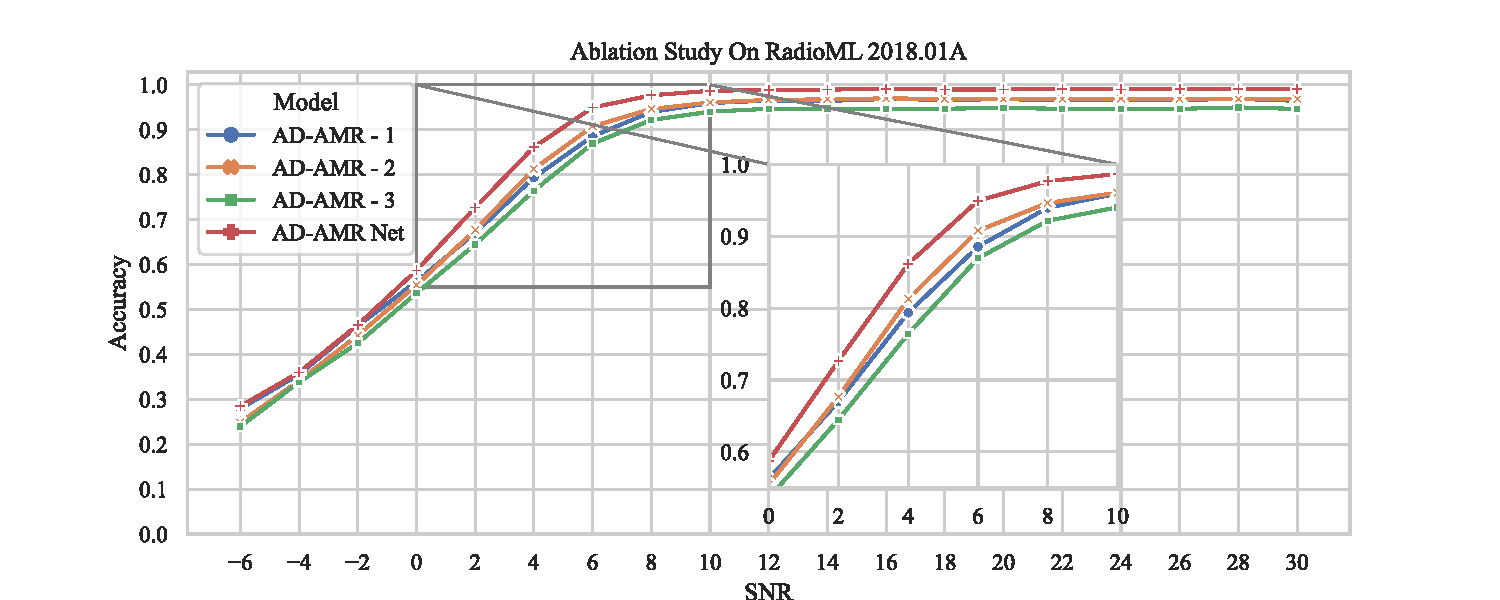
\includegraphics[width=\textwidth]{Image/ablation_res.pdf}
    \caption{消融实验结果}
    \label{fig: ablation_res}
\end{figure}

\begin{table}[ht]
    \caption{讨论结果}
    \begin{center} 
        \resizebox{0.8\textwidth}{!} & +3.29\% & \textbf{+3.51\%}  & \textbf{+6.67\%} & +0.11M \\
                \hline
                ADM-CLDNN & 0.5994 & 0.6126 & 0.5820 & 0.7638 & 1.43M \\
                $\Delta$ & +2.22\% & \textbf{+3.71\%} & +2.32\% & +4.25\% & +0.11M \\
                \hline
                ADM-AWN & 0.6300 & 0.6300 & 0.6139 & 0.8271 & 0.49M \\
                $\Delta$ & +0.38\% & +0.38\% & +0.4\% & +2.35\% & +0.11M \\
                \hline
            \end{tabular}
        }
    \end{center}
~\label{tab: discussion}
\end{table}

\begin{figure}
    \centering
    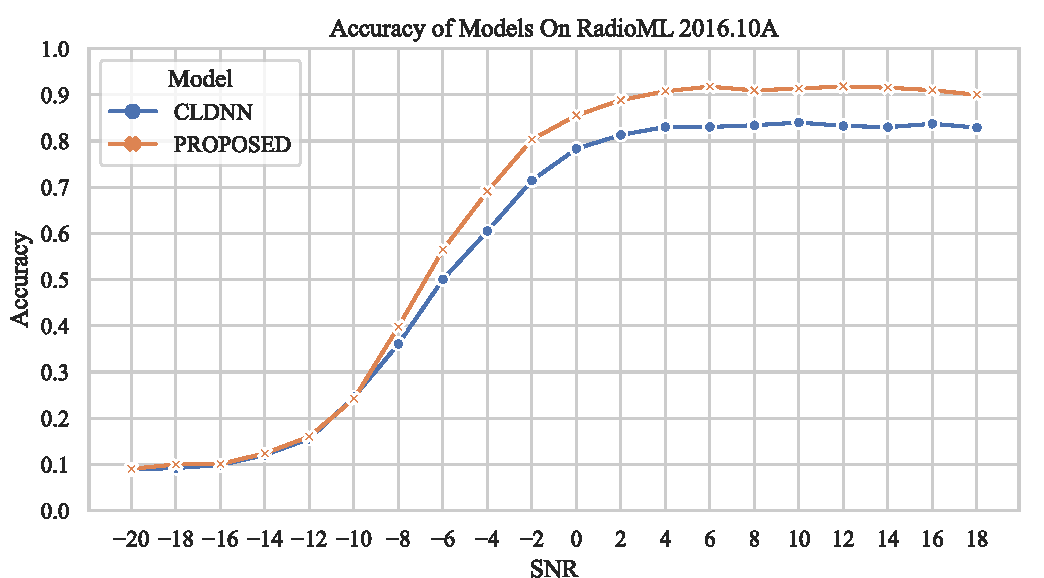
\includegraphics[width=\textwidth]{Image/16a_acc.pdf}
    \caption{不同模型在不同信噪比下的性能比较 (RadioML 2016.10A数据集)}
    \label{fig:2016A_res}
\end{figure}

\begin{figure}[ht]
    \centering
    \begin{subfigure}[b]{0.45\textwidth}
      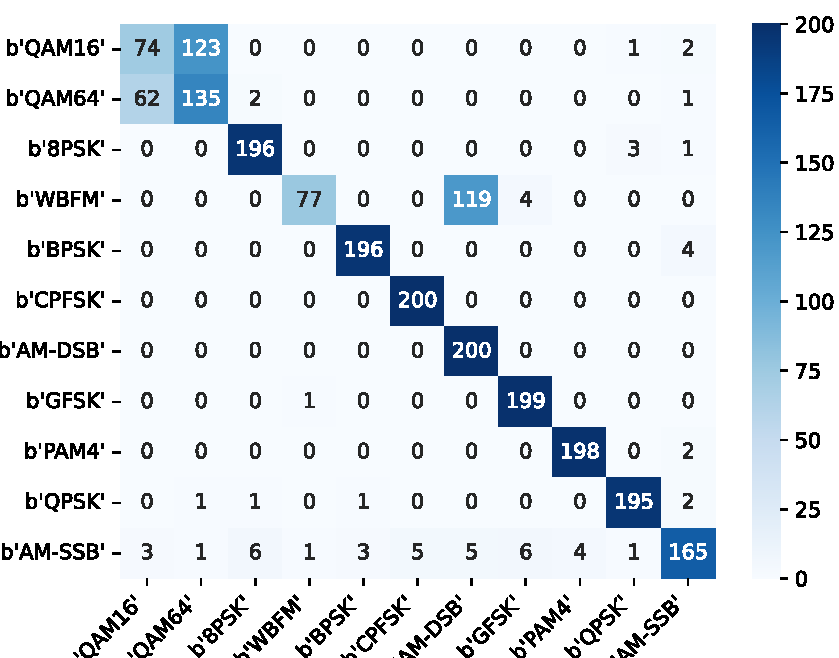
\includegraphics[width=\textwidth]{Image/cldnn_16a.pdf}
      \label{fig:image1}
    \end{subfigure}
    \hfill
    \begin{subfigure}[b]{0.45\textwidth}
      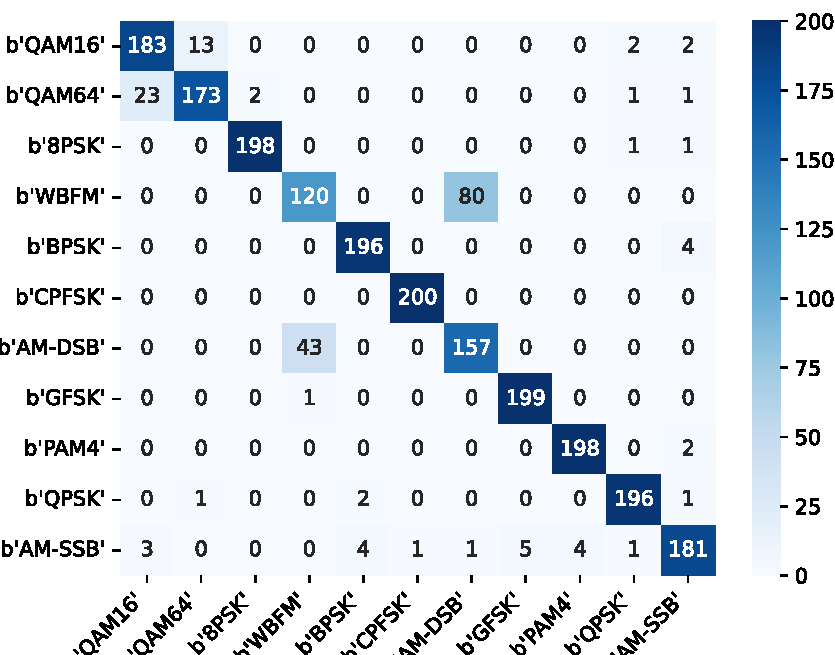
\includegraphics[width=\textwidth]{Image/proposed_16a.pdf}
      \label{fig:image2}
    \end{subfigure}
    \caption{8dB 混淆矩阵 (RadioML 2016.10A数据集, 左:CLDNN, 右:AD-AMR Net)}
    \label{fig:16a_matrix}
  \end{figure}
  
\begin{figure}
    \centering
    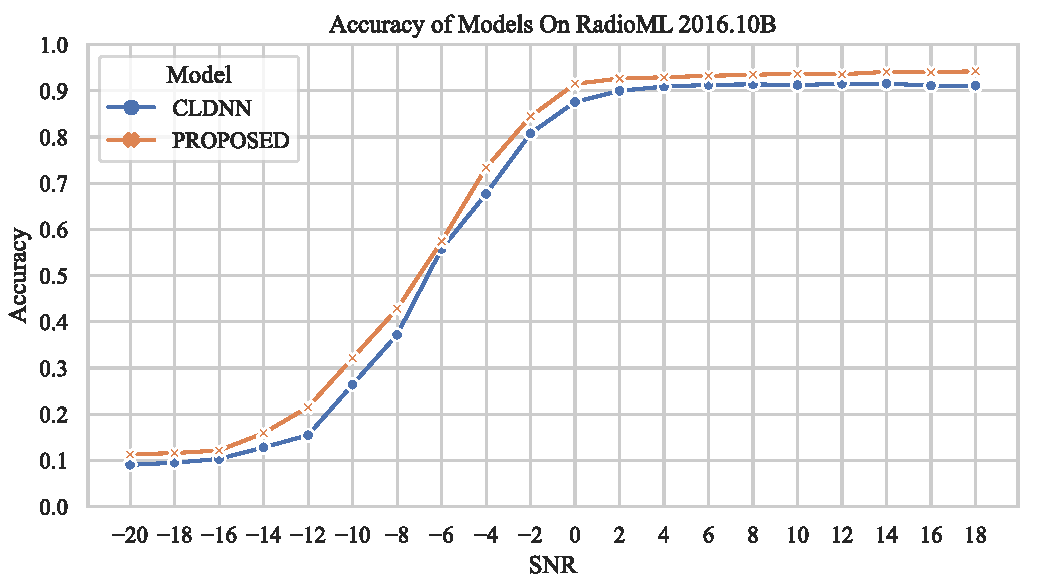
\includegraphics[width=\textwidth]{Image/16b_acc.pdf}
    \caption{不同模型在不同信噪比下的性能比较 (RadioML 2016.10B数据集)}
    \label{fig:2016B_res}
\end{figure}

\begin{figure}[ht]
    \centering
    \begin{subfigure}[b]{0.45\textwidth}
      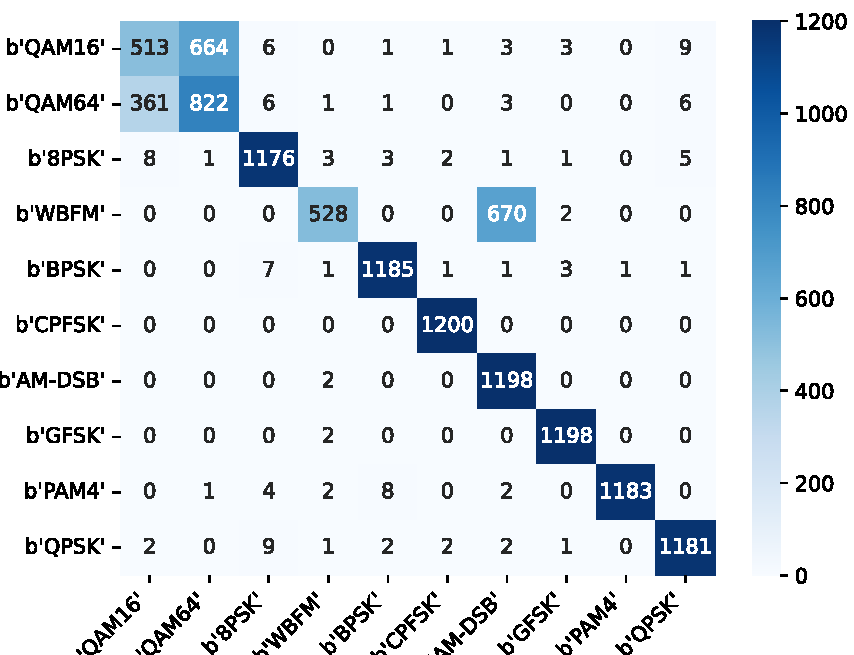
\includegraphics[width=\textwidth]{Image/cldnn_16b.pdf}
      \label{fig:image1}
    \end{subfigure}
    \hfill
    \begin{subfigure}[b]{0.45\textwidth}
      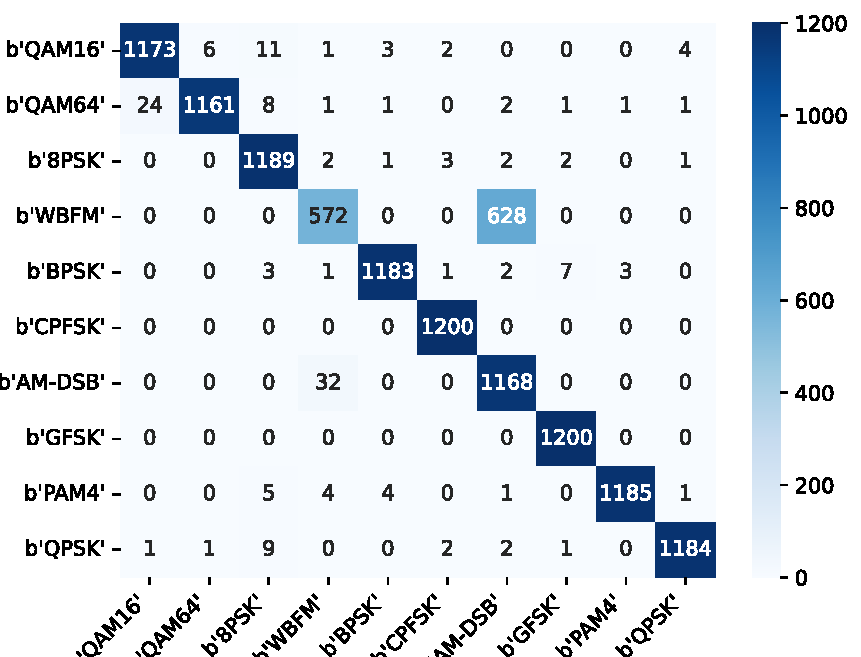
\includegraphics[width=\textwidth]{Image/proposed_16b.pdf}
      \label{fig:image2}
    \end{subfigure}
    \caption{8dB 混淆矩阵 (RadioML 2016.10B数据集, 左:CLDNN, 右:AD-AMR Net)}
    \label{fig:16a_matrix}
  \end{figure}

  \begin{figure}
    \centering
    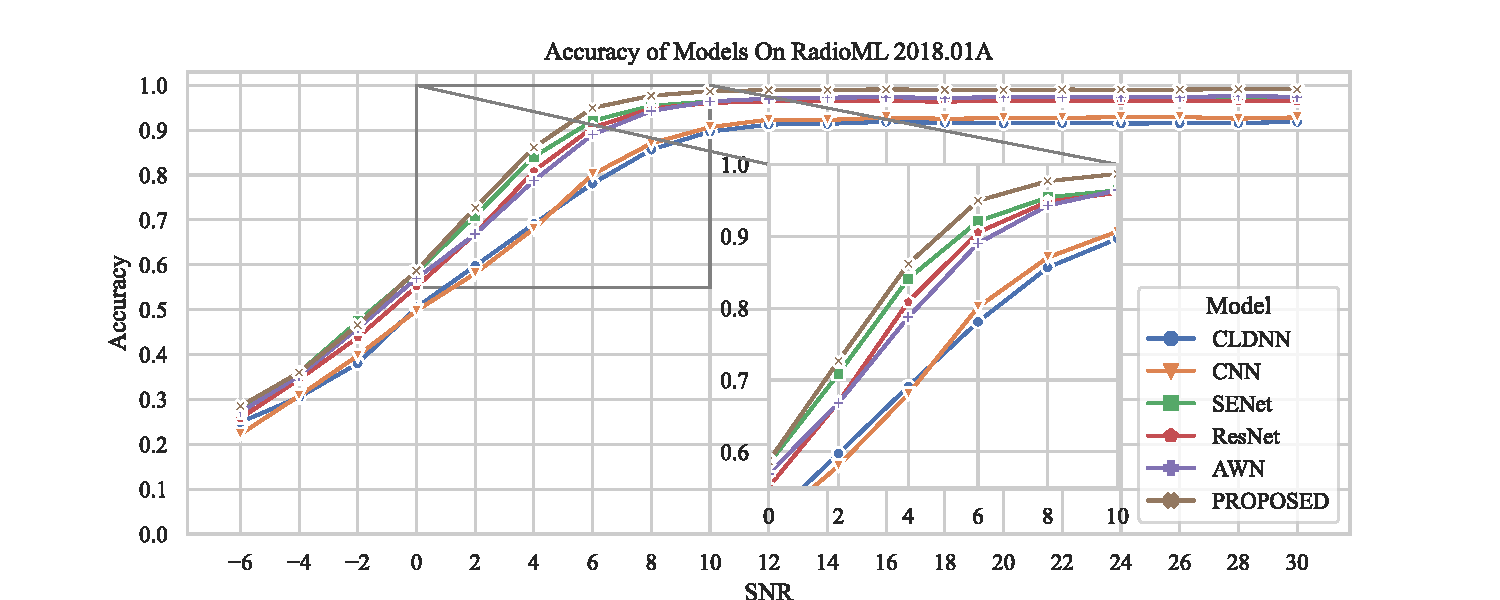
\includegraphics[width=\textwidth]{Image/model_res.pdf}
    \caption{不同模型在不同信噪比下的性能比较 (RadioML 2018.01A数据集)}
    \label{fig:model_acc}
\end{figure}


\begin{figure}[ht]
    \centering
    \begin{subfigure}[b]{0.45\textwidth}
      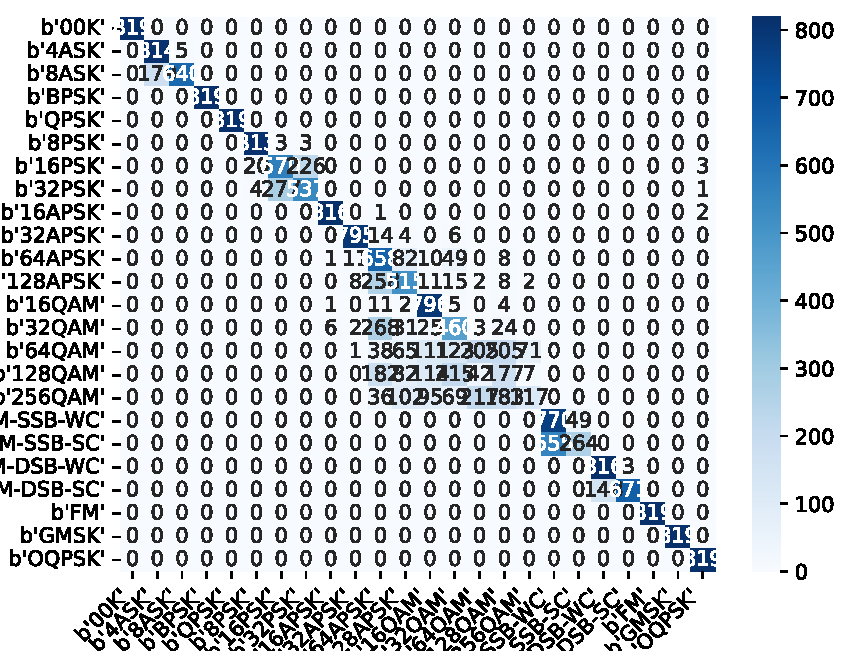
\includegraphics[width=\textwidth]{Image/cldnn_18a.pdf}
      \label{fig:image1}
    \end{subfigure}
    \hfill
    \begin{subfigure}[b]{0.45\textwidth}
      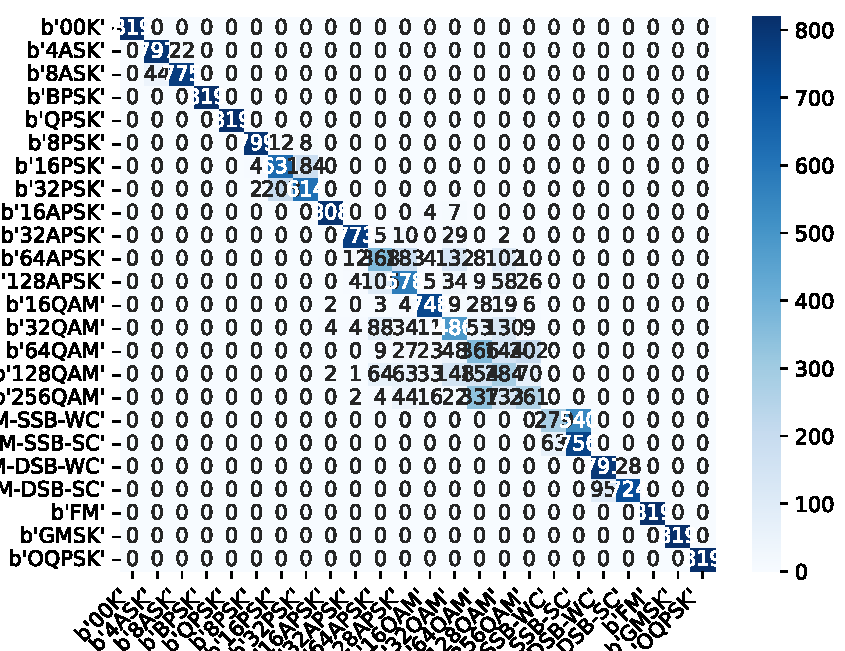
\includegraphics[width=\textwidth]{Image/cnn_18a.pdf}
      \label{fig:image2}
    \end{subfigure}
    \hfill
    \begin{subfigure}[b]{0.45\textwidth}
        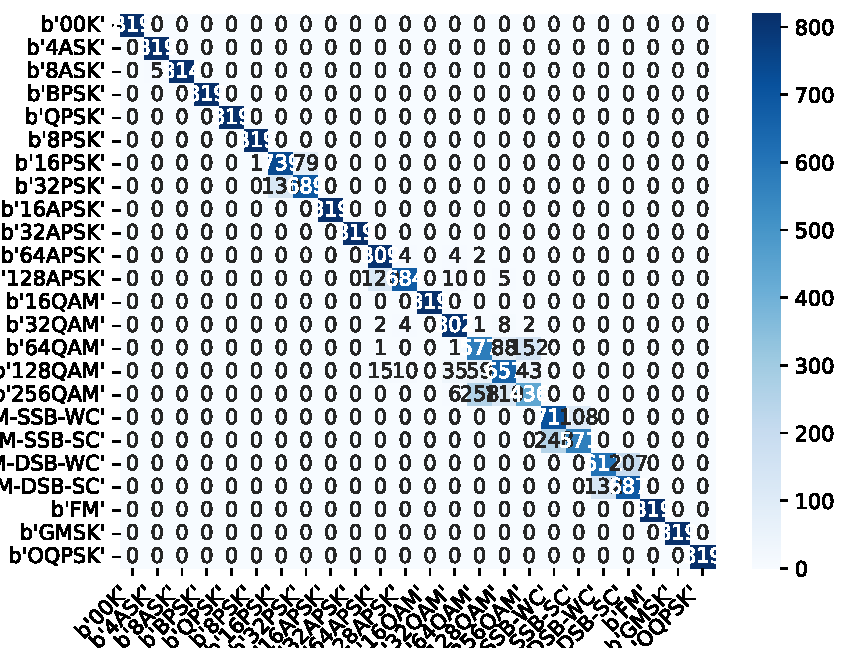
\includegraphics[width=\textwidth]{Image/resnet_18a.pdf}
        \label{fig:image2}
      \end{subfigure}
      \hfill
      \begin{subfigure}[b]{0.45\textwidth}
        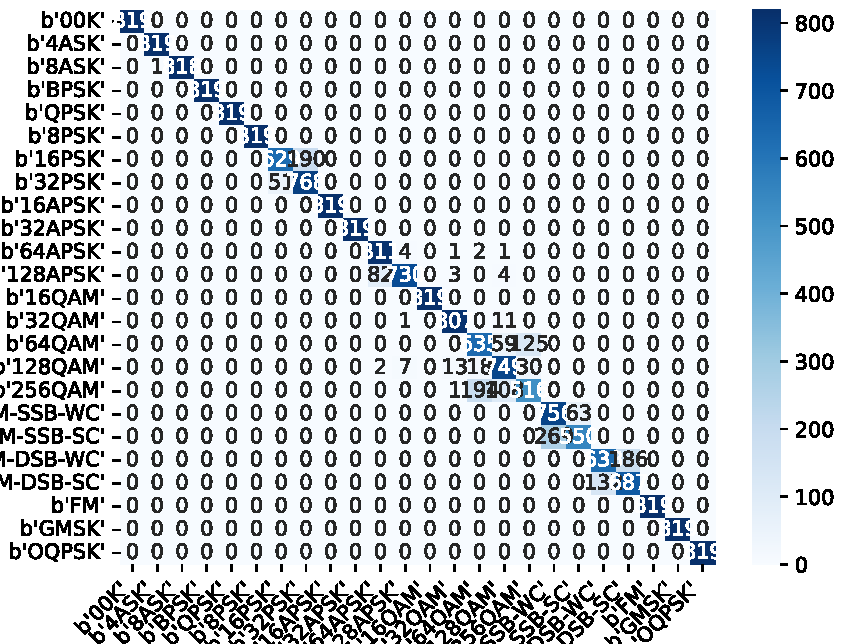
\includegraphics[width=\textwidth]{Image/senet_18a.pdf}
        \label{fig:image2}
      \end{subfigure}
      \hfill
      \begin{subfigure}[b]{0.45\textwidth}
        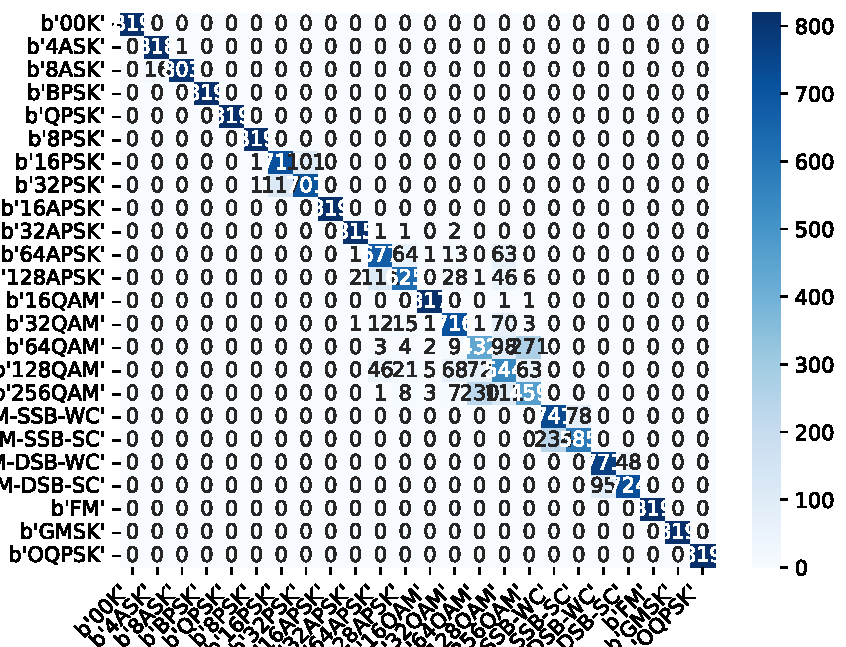
\includegraphics[width=\textwidth]{Image/awn_18a.pdf}
        \label{fig:image2}
      \end{subfigure}
      \hfill
        \begin{subfigure}[b]{0.45\textwidth}
            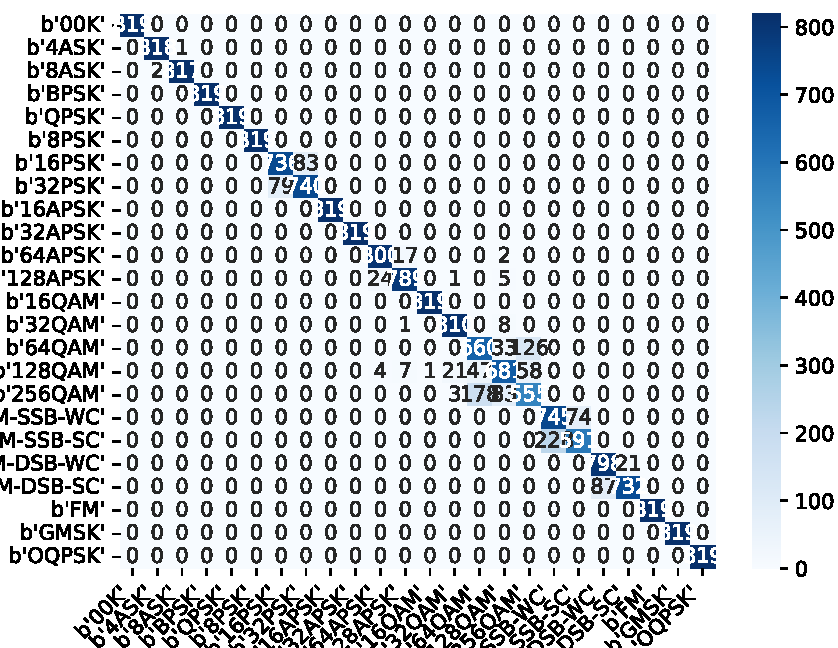
\includegraphics[width=\textwidth]{Image/proposed_18a.pdf}
            \label{fig:image2}
            \end{subfigure}
    \caption{6dB 混淆矩阵 (RadioML 2018.01A数据集, 从左到右,从上到下:CLDNN, CNN, ResNet, SENet, AWN, AD-AMR Net)}
    \label{fig:16a_matrix}
  \end{figure}

在对RadioML 2018.01A数据集进行的实验中,AD-AMR Net模型表现出了明显的性能优势。图~\ref{fig:model_acc}和表~\ref{tab:model_comparison}详细展示了各种模型的性能对比。AD-AMR Net不仅在高信噪比环境中表现优异,更在低信噪比(SNR)环境中展现出了卓越的鲁棒性,这在调制信号识别领域尤为重要。在0~-~10 dB SNR范围内,AD-AMR Net的准确率高达84.8\%,远超其他模型的80~-~82\%。这一显著的性能提升在参数数量显著减少的情况下实现,凸显了模型在效率和性能之间取得了良好的平衡。

我们进一步通过消融实验(表~\ref{tab: ablation})探究了AD-AMR Net内部各组件的作用。去除ADM模块(AD-AMR~-~1)的实验结果显示,性能在所有指标上都有显著下降,特别是在低信噪比条件下,这强调了ADM在提高模型识别能力方面的关键作用。另一方面,仅去除FEM中的ERSB(AD-AMR~-~2)虽然对性能有一定影响,但下降幅度较小。若同时去除这两个核心组件(AD-AMR~-~3),则会导致性能的显著下降,特别是在复杂的信号场景中。这些结果不仅证实了ADM和FEM在提升低信噪比环境下准确性方面的重要性,也突出了它们在维持模型整体性能中的协同作用。

为进一步验证ADM的即插即用特性,我们将ADM应用于其他主流模型,并观察其对性能的影响。如表~\ref{tab: discussion}所示,实验结果表明,不论是在高信噪比还是低信噪比环境下,ADM的加入都能显著提升模型的准确度。这一发现不仅证实了ADM在多种不同环境下的适用性,也展示了它作为一个独立模块对于提高现有模型性能的潜力。

综上所述,通过对AD-AMR Net的全面评估,我们不仅证实了其在多种信噪比环境下的优异性能,也展示了其内部组件的重要性。这些发现为未来调制信号识别模型的设计提供了宝贵的参考,并为进一步提升这类模型的性能和适用性奠定了基础。

\section{本章总结}\label{sec:background}
本章节详细介绍了我们针对自适应噪声矫正调制识别网络(ADM)的一系列实验设计,目的是全面评估ADM在调制识别任务中的性能,并与当前的主流方法进行比较。通过对RadioML 2016.10A、RadioML 2016.10B 和 RadioML 2018.01A三个数据集的深入研究,我们能够在不同规模和复杂性的数据集上测试ADM的有效性。

在实验设计中,我们首先使用较小的RadioML 2016.10A数据集来进行基本的性能比较,特别是与传统的机器学习算法如支持向量机(SVM)进行对比,以验证ADM在基础调制识别任务上的能力。随后,针对更大规模的RadioML 2016.10B数据集,我们将ADM与近年来的深度学习模型如CNN、CLDNN和ResNet进行比较,以评估ADM在处理较复杂数据时的性能。最后,在规模和维度上更大的RadioML 2018.01A数据集上,我们将ADM与当前的主流模型如SENet和AWN进行了比较,进一步验证了ADM在最先进的模型面前的竞争力。

此外,通过一系列消融实验,我们深入分析了ADM中各个组件的作用,特别是ECA模块和ADM模块对整体性能的贡献。这些实验不仅显示了每个单独组件的重要性,也揭示了它们在提升整体模型性能方面的协同作用。在讨论实验中,我们探索了ADM模块的“即插即用”能力,即将其加入到现有模型中的效果,从而展示了ADM模块的通用性和适应性。

综上所述,本章节的实验设计和结果分析为调制识别领域提供了重要的见解,证明了ADM在提升调制识别性能方面的有效性。ADM的成功实施不仅展示了深度学习在解决实际通信问题中的潜力,也为未来在该领域的研究提供了有价值的参考。通过这些实验,我们能够更好地理解深度学习技术在处理复杂信号数据中的应用,以及如何通过创新的模块设计来提升模型性能和效率。

\chapter{宽带调制信号的自动识别}\label{chap:intro}
\markboth{第四章\ \ 宽带调制信号的自动识别}{}
% 宽带亚采样信号的自动识别
% 第四章“宽带亚采样调制信号的自动识别”可以按照以下大纲进行组织:

% 1. **引言**
%    - 介绍研究背景和宽带亚采样调制信号自动识别的重要性。
%    - 阐述研究动机和本章的目的。

% 2. **理论基础和相关工作**
%    - 介绍亚奈奎斯特采样和自动调制识别的基本概念。
%    - 回顾相关领域的研究进展和现有技术。

% 3. **单用户通信场景下的调制识别**
%    - 描述单用户场景的问题设定和挑战。
%    - 介绍使用AD-AMR Net模型进行调制识别的方法和策略。

% 4. **多用户通信场景下的调制识别**
%    - 讨论多用户场景的特点和复杂性。
%    - 介绍三种不同的调制识别方案:直接预测、分步骤方法和多任务学习。

% 5. **实验设计和结果分析**
%    - 描述实验设置、所用数据集和评估指标。
%    - 展示实验结果,并进行详细分析。

% 6. **讨论**
%    - 分析各种方法的优缺点和适用性。
%    - 探讨研究结果对于实际应用和理论发展的意义。

% 7. **结论和未来工作**
%    - 总结本章的主要发现和贡献。
%    - 提出未来研究的方向和可能的改进。

% 这个大纲旨在全面覆盖宽带亚采样调制信号自动识别的关键方面,从理论基础到实际应用,以及从单用户到多用户场景的不同识别策略,为读者提供一个清晰、连贯的研究框架。

% 宽带信号的调制识别可以分为两个方向,一种是只有一个用户在通信的场景,这个时候只需要识别其调制模式即可,另一种是有多个用户在通信的场景,这个时候需要同时识别其所在的子带位置和所使用的调制模式,由第三章的实验,我们提出了一种AD-AMR Net用于调制识别,在这一章节中我们可以将其用作backbone,针对单用户场景只需要对问题进行建模,选择合适的预处理方式,然后在分析性能即可,而多用户场景则比较困难,目前鲜有相关的研究,所以我们需要讨论多种方案,在本章中我们针对该问题采用了三个不同的方案,第一个方案是根据子带的情况和各种调制的可能性,直接预测相应的所有情况,这种方案比较容易实现,可以作为一个基线,第二种方案则是分多步来进行,先识别子带的位置,然后在得到位置信息后进一步进行调制的识别,第三种则是多任务的形式,先总体地对亚采样信号进行特征提取,然后再用不同的head分别实现子带位置的判别和调整模式的识别,与前者不同的是,第三种方案共用了一个特征提取模块,减少了模型的复杂度,同时增加了两个子任务的关联性

\section{引言}\label{sec:background}

在现代通信系统中,频谱资源的有效利用成为了一个关键挑战。随着物联网和无线通信技术的迅速发展,对于高效的频谱利用和信号处理方法的需求日益增长。在这种背景下,亚奈奎斯特采样作为一种有效的频谱感知技术,能够在较低的采样率下捕获宽带信号,减少处理高速信号所需的资源和成本。

自动调制识别在提高通信系统的灵活性和效率方面发挥着重要作用。特别是在多用户通信和动态频谱访问环境中,能够快速准确地识别不同用户的调制方式是至关重要的。然而,当涉及到宽带亚采样信号时,传统的调制识别方法面临着新的挑战,例如如何在降低的采样率下维持识别精度。

在本章节中,我们聚焦于宽带信号的调制识别,这一任务可以分为两个主要方向。首先是单用户通信场景,其中核心任务是识别特定用户的调制模式。针对这一场景,我们利用第三章中提出的AD-AMR Net和主流深度学习模型作为主干网络,通过对问题进行合理的建模和选择适当的预处理方法,进而分析模型在单用户调制识别任务上的性能。

另一方面,我们探讨了更为复杂的多用户通信场景,这一场景不仅要求识别调制模式,还需要确定通信信号的子带位置。由于这一领域的研究相对较少,我们在本章中采用了三种不同的方案来应对这一挑战。第一个方案是直接预测各种可能的子带位置和调制模式的组合,这种方法较为直接,可作为基线模型。第二种方案采用分步骤方法,即先识别子带位置,再基于位置信息进行调制模式的识别。第三种方案则采用多任务学习的形式,通过共享的特征提取模块来同时实现子带位置判别和调制模式识别,这种设计既减少了模型复杂度,也增强了两个子任务之间的关联性。

通过这一章节的研究,我们旨在提供有效的解决方案来应对宽带亚采样调制信号识别中的挑战,同时推动无线通信技术在频谱效率和智能信号处理方面的进步。这不仅对于解决现实世界的通信问题至关重要,也对于理论研究和技术创新具有重要的指导意义。

\begin{figure}
    \centering
    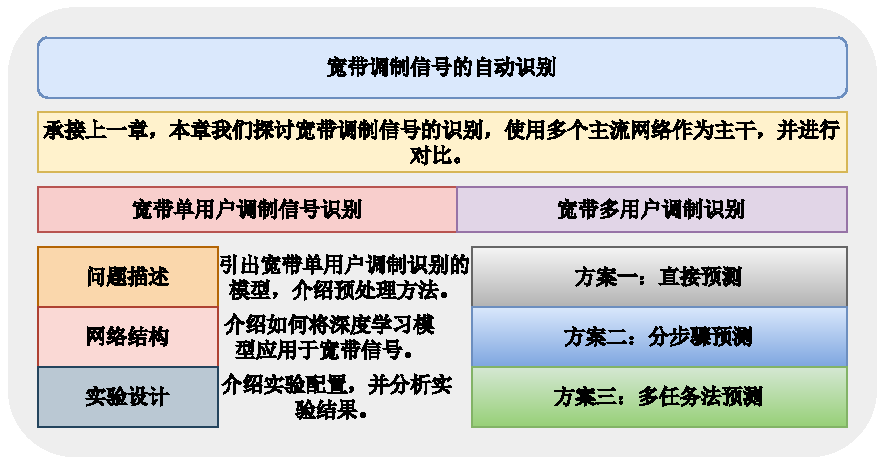
\includegraphics[width=\textwidth]{Image/chap4_map.pdf}
    \caption{本章脉络}
    \label{fig:chap4_overview}
\end{figure}

\section{宽带单用户调制信号识别}\label{sec:background}
% 在撰写单用户场景下的调制识别部分时,您可以按照以下思路来组织内容:

% 1. **问题描述和挑战**:
%    - 介绍单用户通信场景的特点。
%    - 描述在亚奈奎斯特采样条件下进行调制识别所面临的技术挑战。

% 2. **方法论**:
%    - 阐述使用AD-AMR Net进行调制识别的整体方法论。
%    - 详细描述数据预处理、特征提取和分类器设计的步骤。

% 3. **模型架构**:
%    - 详细介绍模型的架构,包括各层的功能和配置。
%    - 插图:提供模型架构的示意图,展示不同层级和组件的关系。

% 4. **实验设置**:
%    - 描述实验的具体设置,包括数据集的选择、模型的训练和评估指标。
%    - 插图:可展示部分样本数据的波形图或频谱图,以帮助理解数据特性。

% 5. **结果分析**:
%    - 展示模型在单用户场景下的识别结果。
%    - 分析模型性能,讨论其在不同条件下的表现。

% 6. **比较与讨论**:
%    - 将AD-AMR Net的性能与其他方法进行比较。
%    - 讨论模型在单用户场景下的优势和局限性。

% 7. **结论**:
%    - 总结在单用户场景下调制识别的主要发现。
%    - 提出可能的改进方向和后续工作的建议。

% 通过这样的结构,您可以系统地介绍单用户场景下调制识别的方法、实验过程和结果分析,为读者提供深入的理解,并展示您的研究成果。

\subsection{问题描述和挑战}\label{sec:background}

\begin{figure}
    \centering
    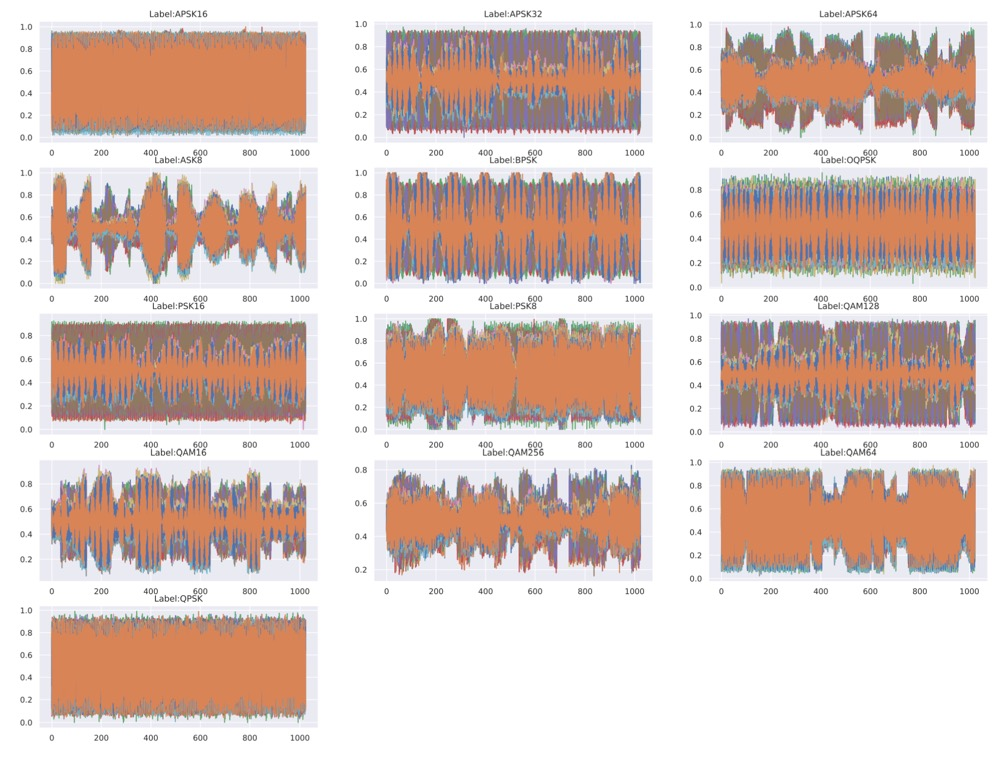
\includegraphics[width=0.8\textwidth]{Image/modulations.jpg}
    \caption{宽带欠采样信号的可视化}
    \label{fig:modulations}
\end{figure}

在宽带单用户调制信号识别的实验研究中,我们集中关注于数据预处理方法、问题建模策略以及AD-AMR Net模型的应用。考虑到亚奈奎斯特采样信号的特点,我们采纳了\textbf{Min-max}预处理方法,\textbf{Min-max}的数学表达式如下:

\begin{equation}
    \boldsymbol{x}_\text{\emph{norm}} = \frac{\boldsymbol{x} - \min(\boldsymbol{x})}{\max(\boldsymbol{x}) - \min(\boldsymbol{x})},
\end{equation}
其中$\boldsymbol{x}_{min}$和$\boldsymbol{x}_{max}$分别表示信号的最小值和最大值。这种方法可以将信号的幅度归一化到$[0, 1]$的范围内,从而保证数据的稳定性和可靠性。以确保在保持数据基本特性的同时,使之适合于神经网络的处理需求。具有不同延迟特性的八个模数转换器(ADC)负责收集输入数据,这些ADC的延迟值为16, 11, 1, 0, 27, 24, 37, 31。这种独特的延迟配置为信号采集引入了额外的复杂性。数据以$I_1, Q_1, I_2, Q_2, ..., Q_8$的顺序排列,构成一个$16 \times 1024$的矩阵,其中I和Q分别表示信号的同相分量和正交分量。此外,我们的研究涵盖了13种调制类型,包括APSK16, APSK32, APSK64, ASK8, BPSK, OQPSK, PSK16, PSK8, QAM128, QAM16, QAM256, QAM64, QPSK等,增加了识别任务的复杂度。宽带欠采样信号的可视化如图\ref{fig:modulations}所示。

在这些背景下,我们面临的主要挑战是有效处理由不同延迟的ADC采集的复杂信号,并从中准确识别出多种可能的调制类型。这不仅要求精确的数据预处理,还需要强大的分类算法,以在降低采样率的条件下实现高精度的调制识别。本章实验设计的目标是分析不同的深度学习模型在处理单用户场景下宽带亚采样信号时的有效性,以及评估其在特定条件下的表现。通过这些实验,我们将深入探索模型在实际应用中的潜力和局限性,为宽带信号的调制识别领域提供新的见解。、

本节中,我们专注于单用户场景下的宽带信号特征提取能力的比较研究。考虑到单用户场景相对简单,它为评估不同深度学习模型在宽带信号处理上的性能提供了一个理想的测试环境。为此,我们选取了多种主流的深度学习模型进行比较,包括传统的ResNet、加入了卷积层注意力模块(Convolutional Block Attention Module, CBAM)的ResNet、融合了自注意力机制的卷积神经网络、加入了残差收缩模块(Residual Shrinkage Block)的ResNet,以及第三章中提出的集成了高效通道注意力的残差收缩模块的ResNet。通过这一系列的比较分析,我们可以深入理解每个模型在宽带信号特征提取方面的优势和局限,为自动调制识别技术的发展提供新的见解。

\subsection{网络结构}\label{sec:background}


\begin{figure}
    \centering
    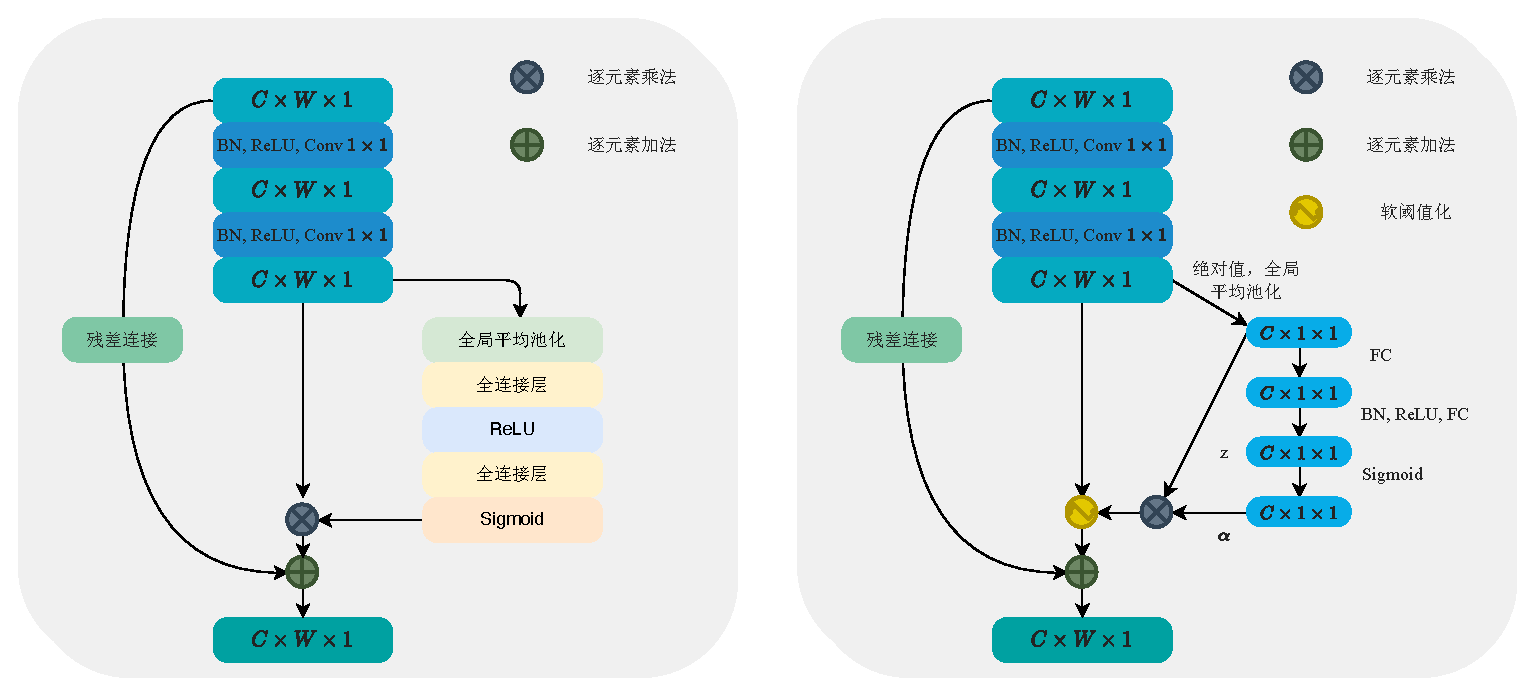
\includegraphics[width=\textwidth]{Image/se_rsb_cn.pdf}
    \caption{挤压-激励模块(左)和残差收缩模块(右)}
    \label{fig:se_rsb}
\end{figure}

\subsubsection{挤压-激励模块}\label{sec:background}
在深度学习领域,特别是在图像识别和信号处理任务中,注意力机制的引入已经证明可以显著提升模型的性能。挤压-激励模块(Squeeze-and-Excitation, SE)是一种有效的注意力机制实现,它通过重新校准卷积层的特征通道的响应强度,增强了模型对于重要特征的关注度,同时抑制了不重要的特征。SE模块的核心思想是先对特征图进行全局平均池化(Squeeze),从而生成特征通道的全局描述,然后通过两个全连接层(Excitation)对这些描述进行重标定,最终通过缩放原始特征图来实现特征的重新校准。这个过程可以表示为:

\begin{equation}
    \textbf{S}(z) = \frac{1}{H \times W} \sum_{i=1}^{H} \sum_{j=1}^{W} z_{i,j}
\end{equation}
\begin{equation}
    \textbf{E}(s) = \sigma(g(s, \textbf{W})) = \sigma(\textbf{W}_2 \delta(\textbf{W}_1 s))
\end{equation}
\begin{equation}
    \tilde{x}_c = F_{scale}(x_c, e_c) = e_c \cdot x_c
\end{equation}

其中,\(z\) 是输入特征图,\(\textbf{S}(z)\) 表示Squeeze操作后的全局特征,\(\textbf{E}(s)\) 是Excitation操作后的权重系数,\(\sigma\) 表示sigmoid激活函数,\(g\) 表示全连接层操作,\(\textbf{W}_1\) 和 \(\textbf{W}_2\) 是全连接层的权重,\(\delta\) 表示ReLU激活函数,\(e_c\) 是每个通道的重标定权重,\(\tilde{x}_c\) 是最终的输出特征图,\(F_{scale}\) 表示特征缩放函数。

为了将SE模块应用于一维信号处理任务中,特别是调制识别,我们对其进行了适当的修改,将原本针对二维图像特征的处理改为适用于一维信号。这意味着在Squeeze阶段,我们采用一维全局平均池化而不是二维平均池化,以正确地处理一维信号数据。这种改进使得SE模块能够有效地处理一维信号特征,通过学习到的通道权重来强调重要的信号特征并抑制不相关的噪声或信息,从而提高了调制识别任务的性能。

将SE模块运用于该任务上,我们的理念是利用其通道注意力机制来增强神经网络对一维信号中重要特征的捕捉能力,进一步提升调制识别的准确性。通过对一维信号特征的有效校准,我们能够实现对信号中调制特征的更加精确识别,这对于提高无线通信系统中的信号处理性能至关重要。

\subsubsection{残差收缩模块}\label{sec:background}
在深度探索深度学习模型在信号处理领域,特别是调制识别任务的应用中,残差收缩模块(Residual Shrinkage Block, RSB)凭借其独特的优势成为研究的焦点。该模块,如图\ref{fig:se_rsb}所示,通过整合残差连接和特征收缩机制,显著优化了网络的特征学习流程并增强了特征表达能力,使得RSB在复杂信号处理任务中展现出非凡的性能。

RSB模块的一大创新在于其对软阈值化技术的应用,这是信号处理中一种常用的工具,特别适合于处理含有噪声的信号。软阈值化通过设置一个阈值来减少信号中的小波系数,有效地去除噪声同时保留信号的主要特征。这一过程中,阈值的选择至关重要——过高会导致信号的过度平滑,损失有价值信息;而过低则可能无法充分去除噪声。RSB通过融入神经网络,能够自适应地学习和调整软阈值化中的阈值参数,从而在去噪和特征保留之间实现最佳平衡。

这种自适应的软阈值化机制,使得RSB在处理宽带信号调制识别任务时尤其有效。宽带信号常包含复杂的调制特征和背景噪声,RSB能够有效地从这些信号中提取出关键信息,抑制不必要的干扰,进而提高调制识别的准确度和鲁棒性。动态调整特征通道,加之其强化关键特征的学习能力,使RSB在复杂信号处理中显示出优越的性能。

正是基于RSB在特征提取、信息压缩及网络训练稳定性方面的显著优势,以及其在软阈值化应用中的自适应能力,我们选择将其作为对比研究对象之一。此项比较旨在全面评估RSB模块在宽带信号处理,尤其是调制识别任务中的表现。通过这种方式,我们不仅能够验证RSB模块的实际效用,也为深度学习模型处理高复杂度信号的未来研究提供新的视角和方法。

\subsubsection{卷积层注意力模块(CBAM)}\label{sec:background}

\begin{figure}
    \centering
    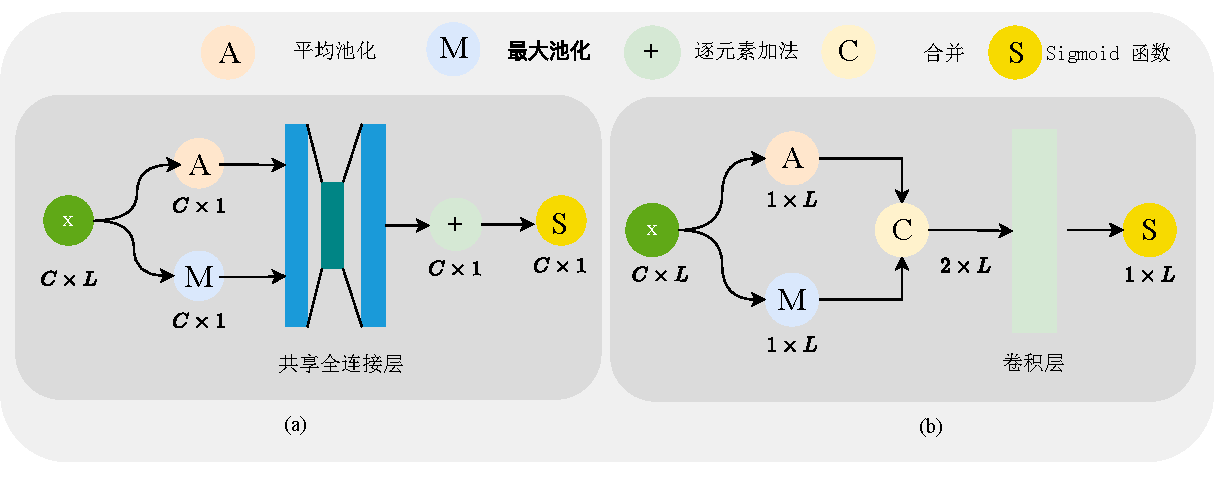
\includegraphics[width=\textwidth]{Image/CBAM_cn.pdf}
    \caption{卷积块注意力模块(CBAM)}
    \label{fig:cbam}
\end{figure}

CBAM(Convolutional Block Attention Module)图\ref{fig:cbam}是一种用于增强神经网络特征表达能力的注意力机制模块。它通过对输入特征图进行细致的分析,有效地强调了对任务有益的特征,从而提升了网络的整体性能。CBAM的核心设计理念是在通道和空间两个维度上应用注意力机制,以此优化网络的特征学习过程\cite{woo2018cbam}。

通道注意力机制关注于识别并强调那些对最终识别任务最重要的通道。它通过全局平均池化和最大池化操作来捕获通道间的全局信息,然后通过多层感知机(MLP)和激活函数来生成通道注意力权重。这个过程可以理解为一种自动的特征选择机制,使网络更加专注于有助于任务的特征通道。通道注意力的计算公式如下:

\begin{equation}
    \begin{aligned}
    M_c(F) &= \sigma(MLP(AvgPool(F)) + MLP(MaxPool(F))) \\ 
    &= \sigma(W_1(W_0(F_{avg}^c)) + W_2(W_0(F_{\max}^c)),
    \end{aligned}
    \label{equ:CAM}
\end{equation}
其中$F$表示输入特征图,$F_{avg}^c$和$F_{\max}^c$分别表示$F$的通道$c$的平均池化和最大池化结果,$W_0$和$W_1$表示两个MLP的权重矩阵,$\sigma$表示激活函数,$M_c(F)$表示通道注意力权重。通过这种方式,网络可以自动学习到每个通道的重要性,从而提高特征的表达能力。

空间注意力机制则集中于特征图的特定空间区域。它通过池化操作来总结特征图的空间信息,并通过一个小型的卷积层来生成空间注意力图。这一机制有助于突出重要的空间区域,使网络能够更加关注于对分类或其他任务有利的空间特征。空间注意力的计算公式如下:

\begin{equation}
    \begin{aligned}
    M_s(F) &= \sigma(f^{7}([AvgPool(F), MaxPool(F)])) \\
    &= \sigma(f^{7}([F_{avg}^s, F_{\max}^s])
    \end{aligned}
    \label{equ:SAM}
\end{equation}
其中$F_{avg}^s$和$F_{\max}^s$分别表示$F$的平均池化和最大池化结果,$f^7$表示一个$7 \times 7$的卷积层,$M_s(F)$表示空间注意力权重。通过这种方式,网络可以自动学习到每个空间区域的重要性,从而提高特征的表达能力。

\begin{figure}
    \centering
    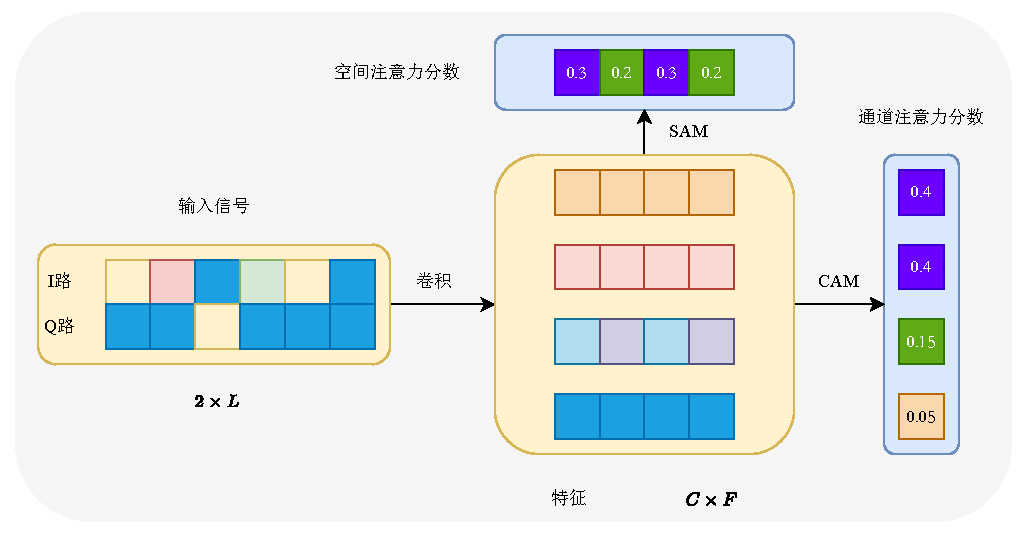
\includegraphics[width=\textwidth]{Image/cbam_on_iq.pdf}
    \caption{卷积块注意力模块用于IQ信号的特征提取}
    \label{fig:cbam_iq}
\end{figure}

原始的CBAM设计是针对二维特征图的,主要用于计算机视觉领域。为了适应一维的信号处理任务,例如调制识别,CBAM模块经过了适当的修改。在这种情况下,CBAM的设计需要考虑信号的时域特性,并根据一维数据的结构进行调整。例如,通道注意力机制可以专注于不同时间窗口内的信号特征,而空间注意力机制则可以针对信号的不同部分进行加权,这对于捕获时间序列数据的重要模式尤为关键。图\ref{fig:cbam_iq}展示了卷积模块注意力机制在处理IQ信号时的大概过程,旨在通过计算空间注意力分数和通道注意力分数来增强模型对信号的识别能力。图中首先展示了输入信号,分为I路和Q路,这两路信号代表了复信号的实部和虚部,是无线通信中常用的信号表示方法。
在经过初步的卷积操作后,模型分别对处理过的信号应用了空间注意力机制和通道注意力机制。空间注意力机制(SAM)通过聚焦于信号中最重要的空间区域来增强特征表达,其注意力分数如图中所示,是通过评估信号各部分的重要性后得到的权重分布,例如0.3、0.2等。这种机制能够使模型更加关注于信号中具有较高信息含量的区域。通道注意力机制(CAM)则关注于不同通道(在本例中可以理解为I路和Q路信号的不同特征通道)的重要性,通过为每个通道分配一个注意力分数(如图中的0.4、0.15、0.05)来实现。这允许模型对不同的特征通道进行重标定,从而强化重要通道的特征而抑制不重要通道的特征。整个过程最终导致了对输入IQ信号特征的有效提炼和加强,使得模型能够更加准确地识别和处理信号。

CBAM的优点在于其模块化和灵活性。它可以轻松地嵌入到现有的卷积神经网络中,无需对网络架构进行大规模修改。此外,CBAM对于不同类型的神经网络,如ResNet或CNN,都有良好的兼容性。在应用于一维信号处理任务时,CBAM提供了一种有效的方式来增强网络对时间序列数据的理解能力,从而提高整体性能。

\subsubsection{自注意力与多头自注意力机制}\label{sec:background}

\begin{figure}
    \centering
    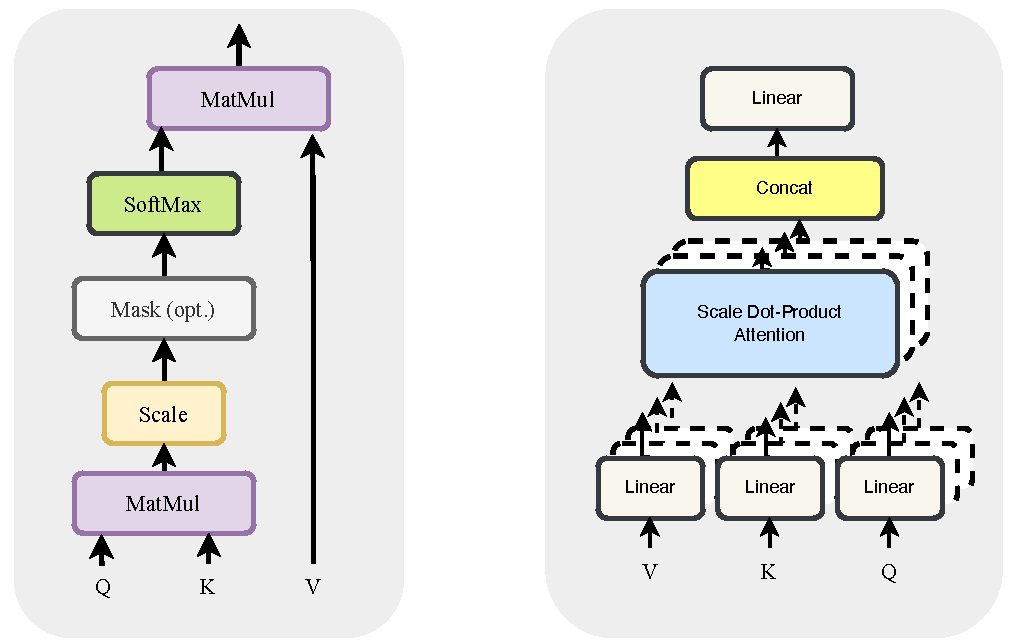
\includegraphics[width=\textwidth]{Image/self-attention.pdf}
    \caption{自注意力与多头自注意力机制}
    \label{fig:self-attention}
\end{figure}

自注意力机制和多头自注意力机制图\ref{fig:self-attention}是深度学习中用于增强模型处理序列数据能力的重要技术。这些机制在处理如自然语言和复杂信号等序列数据时尤为有效。

自注意力机制的核心在于允许模型在处理序列中的每个元素时,同时考虑序列中的所有其他元素。这种机制通过计算序列中每个元素与其他元素之间的关系强度来实现,从而使模型能够更好地理解和表示序列数据。具体来说,自注意力机制通过计算“查询”(Query)、“键”(Key)和“值”(Value)三个向量的相互作用来实现,这些向量是通过对输入数据的不同变换得到的。自注意力的计算过程涉及到这些向量间的点乘操作,然后通过softmax函数进行归一化,从而得到不同元素间的注意力权重。通过这种方式,模型可以更加关注与当前处理元素最相关的其他元素。其计算公式如下:

\begin{equation}
    \text{Attention}(Q, K, V) = \text{softmax}(\frac{QK^T}{\sqrt{d_k}})V,
\end{equation}
其中$d_k$表示“键”向量的维度。

多头自注意力机制则是在此基础上的拓展。它包含多个自注意力“头”,每个头都执行自注意力操作,但使用不同的参数。这样,模型可以从不同的表示子空间中学习信息,从而获得更加全面和丰富的数据表示。每个头的输出会被合并并通过一个线性层进行转换,以产生最终的输出。这种设计使得模型可以在多个维度上捕获序列数据的特征,从而增强了模型的表达能力。其计算公式如下:

\begin{equation}
    \text{MultiHead}(Q, K, V) = \text{Concat}(\text{head}_1, ..., \text{head}_h)W^O,
\end{equation}
其中$\text{head}_i = \text{Attention}(QW_i^Q, KW_i^K, VW_i^V)$,$W_i^Q, W_i^K, W_i^V$和$W^O$分别表示第$i$个头的“查询”、“键”、“值”和输出的线性变换矩阵。

在宽带信号调制识别的应用中,这些机制尤为重要。自注意力和多头自注意力机制可以帮助模型更有效地处理和分析宽带信号中的复杂模式和结构,如频率变化、时间依赖性等。通过这些机制,模型能够更准确地识别不同的调制类型和信号特性,即使在信噪比较低或者信号受到干扰的情况下也是如此。因此,我们将这些机制应用于宽带信号调制识别的任务中,以研究它们对于提高模型性能的作用。


\begin{figure}
    \centering
    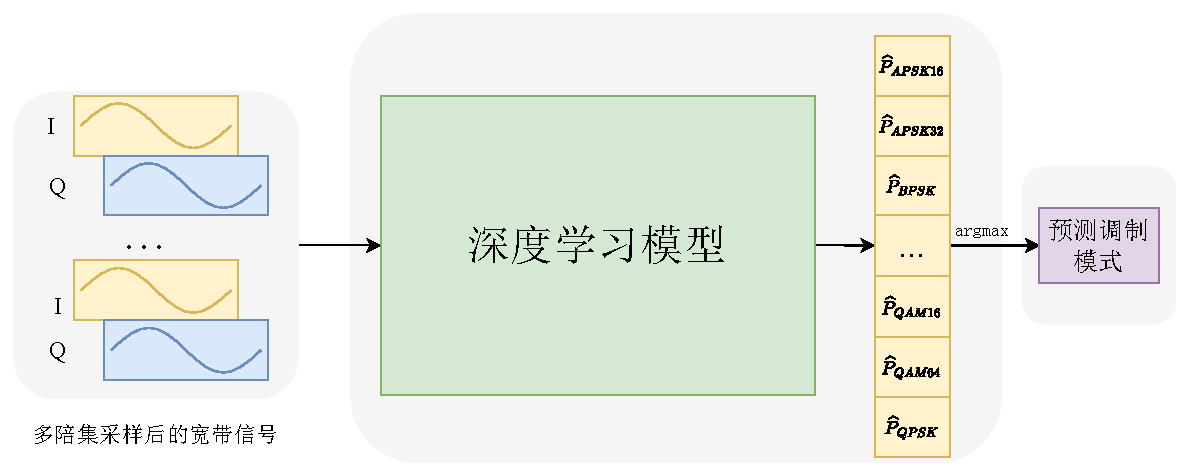
\includegraphics[width=\textwidth]{Image/adamr-wideband.pdf}
    \caption{单用户通信场景下的调制识别网络结构}
    \label{fig:basic}
\end{figure}

\subsection{实验设置}\label{sec:background}

本实验的目的是评估和比较不同模型在调制识别任务上的性能。我们选择了基于PyTorch框架在Ubuntu系统上进行的实验,并使用了NVIDIA RTX 3090 GPU来加速模型训练过程。实验数据集采用的是专为调制识别设计的GBSense 2022 Basic,它包含了多种调制类型的信号样本。

为了确保实验的公平性,我们设定了以下实验条件:

\begin{itemize}
    \item \textbf{对比模型}:我们以ResNet作为基线模型,并评估了几种主流的注意力机制模块——SE模块、RSB模块、CBAM模块、多头自注意力机制模块,以及我们自行提出的AD-AMR Net。这样做是为了观察这些模型在调制识别任务上的性能表现。
    \item \textbf{实验平台}:实验在Ubuntu操作系统上,基于PyTorch框架执行。我们利用NVIDIA RTX 3090 GPU加速了训练过程,以提高实验效率。
    \item \textbf{数据集}:使用GBSense 2022 Basic数据集进行训练、验证和测试,数据集被划分为训练集(60\%)、验证集(20\%)和测试集(20\%)。
    \item \textbf{训练细节}:所有模型都将被训练100个epochs,以确保足够的学习。我们引入了早停机制(Early Stopping)以防过拟合,以及平台期衰减学习率(ReduceLROnPlateau)机制,以自适应调整学习率,确保有效的学习率调整。
    \item \textbf{优化器与损失函数}:在训练过程中,我们采用了随机梯度下降(SGD)优化器,并使用交叉熵损失函数(Cross-Entropy Loss)作为模型训练的损失函数,这有助于处理分类问题中的多类标签。
\end{itemize}

\subsection{评价指标}

模型的性能将基于以下关键指标进行评估:

\begin{itemize}
    \item \textbf{模型参数量}:反映模型复杂度的指标,较少的参数量意味着模型更为简洁。
    \item \textbf{训练至收敛的Epoch数}:衡量模型训练效率的指标,较少的Epoch数表示模型训练所需时间更短。
    \item \textbf{最终准确率}:衡量模型性能的主要指标,在测试集上的准确率越高,表示模型性能越好。
\end{itemize}

通过这些评价指标,我们不仅能够客观比较各模型的性能,还能深入分析各种注意力机制在调制识别任务中的实际应用效果和价值。


\subsection{结果分析}\label{sec:background}

\begin{figure}
    \centering
    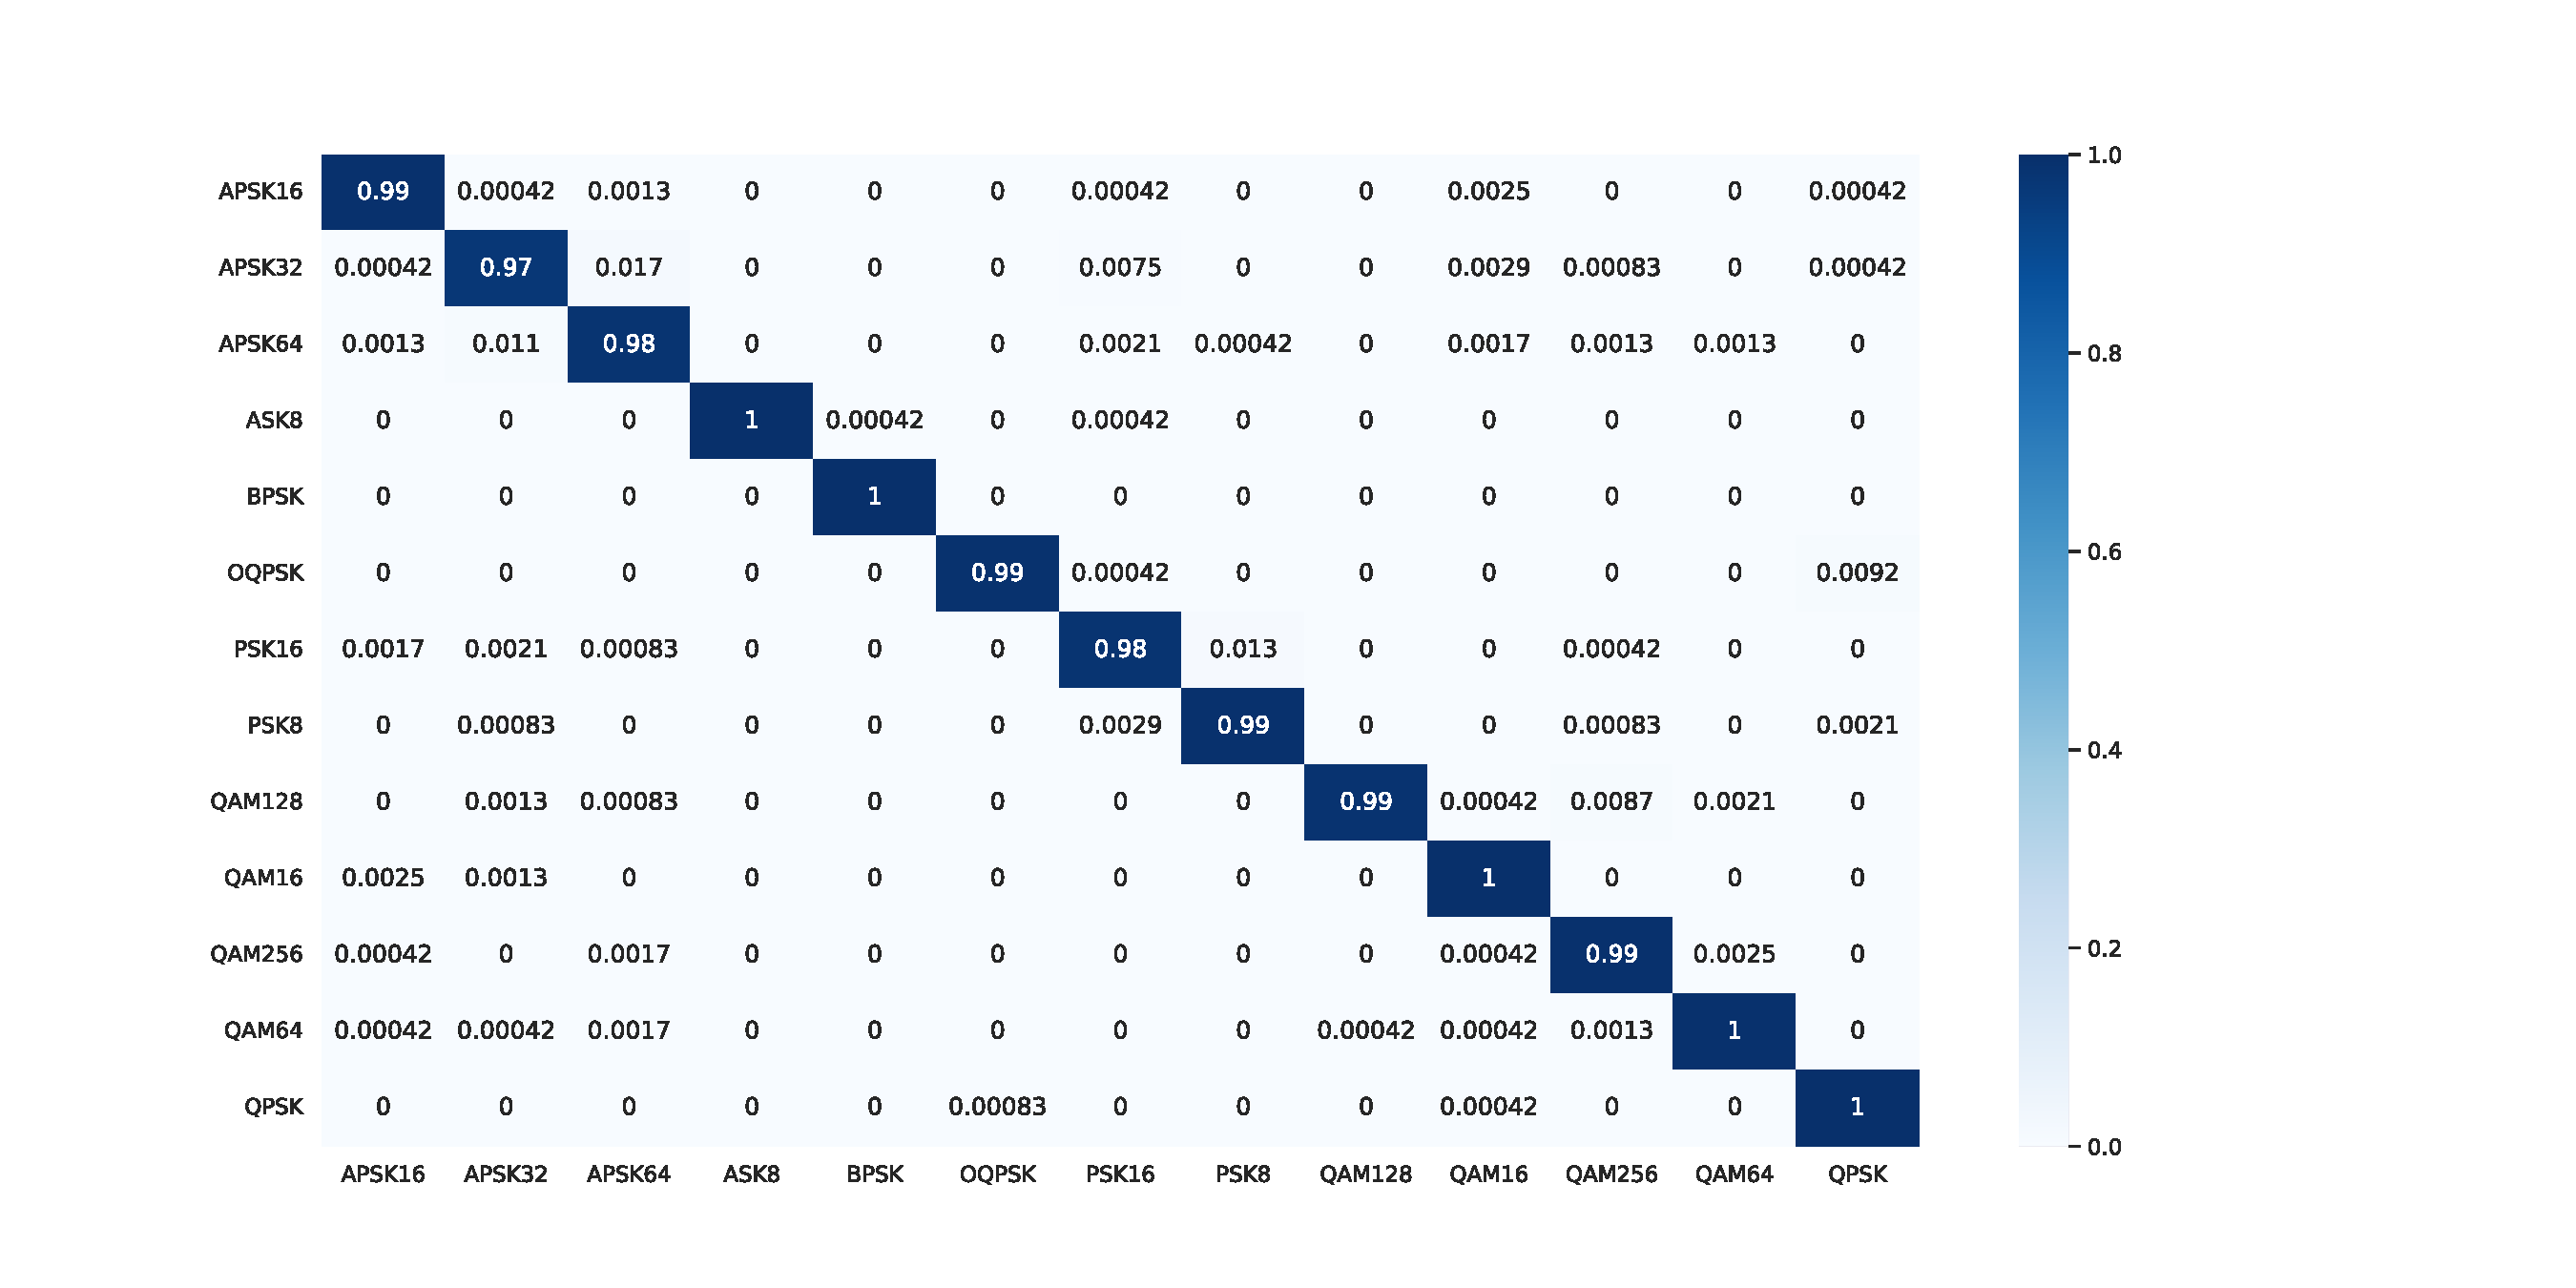
\includegraphics[width=\textwidth]{Image/confusion_matrix.pdf}
    \caption{单用户通信场景下的混淆矩阵(ResNet)}
    \label{fig:basic_result}
\end{figure}

\begin{table}[ht]
    \centering
    \caption{不同模型的性能比较}
    \label{tab:model_comparison}
    \begin{tabular}{lccc}
    \hline
    \textbf{模型}          & \textbf{参数量} & \textbf{训练至收敛的Epoch数} & \textbf{最终准确率} \\ \hline
    ResNet                 & 7.6M             & 68                           & 97.3\%              \\
    SE模块                 & 7.83M             & 57                           & 98.8\%              \\
    RSB模块                & 8.12M             & 54                           & 98.9\%              \\
    CBAM模块               & 7.96M           & 67                           & 98.5\%              \\
    多头自注意力机制模块 & 13.4M             & 99                          & 96.2\%              \\
    AD-AMR Net             & 1M            & 43                           & 99.8\%              \\ \hline
    \end{tabular}
    \label{tab:model_comparison_single_wideband}
\end{table}
    
从表\ref{tab:model_comparison_single_wideband}中提供的性能比较数据可以看出,不同模型在调制识别任务上的表现各有卓越。ResNet作为基线模型,已经展现了相当高的准确率(97.3\%),这验证了深度残差网络在特征提取方面的有效性。然而,通过引入注意力机制的模型在多数情况下能够实现更好的性能。

具体来说,SE模块和RSB模块以较小的参数增加(分别为7.83M和8.12M)实现了显著的性能提升,最终准确率分别达到了98.8\%和98.9\%。这表明通过重标定通道的重要性,可以更有效地利用模型的参数,从而提高准确率。CBAM模块虽然在参数量上仅略有增加(7.96M),但也展现出了良好的性能提升(最终准确率为98.5\%),证明了空间注意力和通道注意力的结合在提高模型敏感度方面的有效性。

多头自注意力机制模块的参数量显著增加至13.4M,但训练至收敛的Epoch数最高(99),且最终准确率相对较低(96.2\%)。这可能是因为该模块在处理一维信号时的参数并没有得到充分有效的利用,或者模型过于复杂导致过拟合。

显著地,我们提出的AD-AMR Net以极低的参数量(仅1M)和较快的训练速度(43 Epochs至收敛)达到了最高的准确率(99.8\%)。这一结果强调了AD-AMR Net在设计上的高效性和在调制识别任务上的出色性能,显示了在模型设计时对参数效率和网络结构优化的重要性。

总体而言,这些结果表明,通过引入针对性的注意力机制,可以在不显著增加参数量的情况下提升模型的性能。特别是,AD-AMR Net的优异表现证明了在保持模型轻量化的同时实现高准确度是可能的,这对于需要部署在资源受限环境中的调制识别系统尤为重要。
\section{宽带信号多用户调制识别}\label{sec:background}

% 在撰写宽带信号多用户调制识别这一章节时,您可以按照以下思路进行:

% 1. **多用户场景下的问题描述**:首先,详细介绍在多用户通信环境中识别调制信号的复杂性和技术挑战,特别是亚采样信号处理的复杂性。

% 2. **三种不同的解决方案**:
%    - **方案一(基线模型)**:根据子带的情况和各种调制的可能性,直接预测所有情况。简介该方案的实现及其作为基线的意义。
%    - **方案二(分步骤识别)**:首先识别子带的位置,然后在获取位置信息后进一步进行调制的识别。解释这种方法的步骤和预期效果。
%    - **方案三(多任务学习)**:总体对亚采样信号进行特征提取,然后使用不同的head分别进行子带位置的判别和调制模式的识别。阐述这种方案如何通过共用特征提取模块减少模型复杂度,同时增加两个子任务的关联性。

% 3. **实验设计和评估**:详细描述用于测试这三种方案的实验设计,包括数据集的选择、评估标准和实验流程。

% 4. **结果分析和比较**:展示每种方案的实验结果,并进行比较分析,以评估各方案的效果和适用性。

% 5. **讨论**:讨论所观察到的趋势和结果,探讨可能的改进方向和未来工作。

% 通过这样的结构,可以全面而深入地探讨多用户场景下宽带信号调制识别的各种策略和方法,展示实验研究的深度和广度。

\subsection{问题描述}\label{sec:background}

\begin{figure}
    \centering
    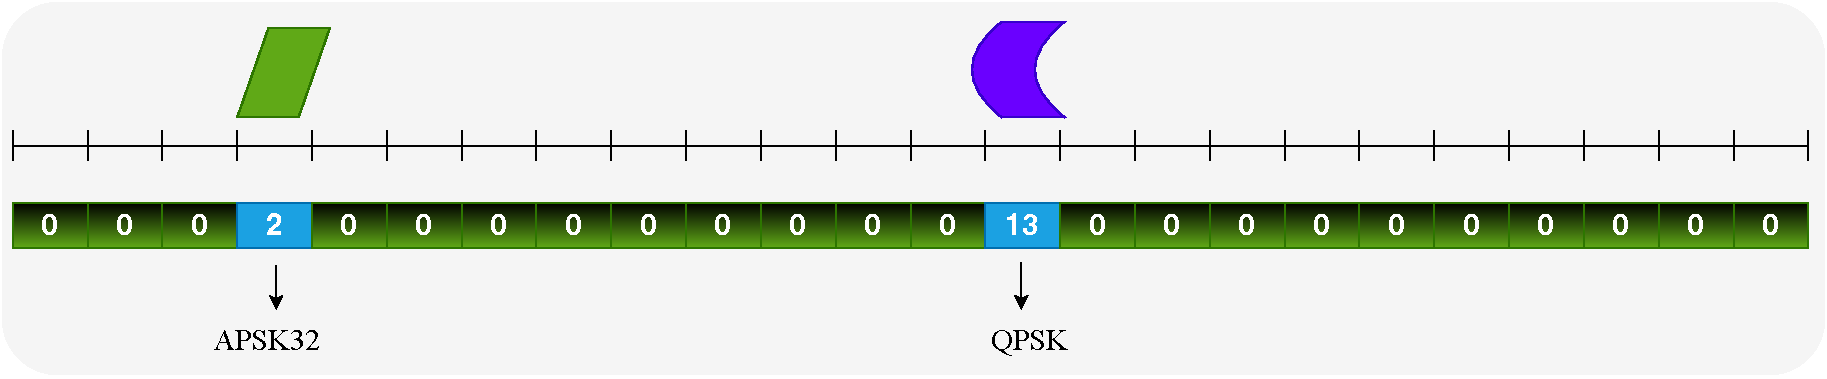
\includegraphics[width=\textwidth]{Image/mods.pdf}
    \caption{多用户通信场景下的调制识别问题描述}
    \label{fig:problem_description}

\end{figure}

在宽带多用户调制识别的问题描述中,我们面对一个复杂的通信环境,其中多个用户可能在相同或重叠的频率范围内同时传输信号。如图\ref{fig:problem_description}所示,这些信号可以被看作是分布在不同子带上的多个通道,每个通道可能采用不同的调制。例如,图展示了编号为2和13的两个子带正在被使用,而其他子带则处于空闲状态。在这种场景下,我们的目标是不仅识别出哪些子带正在被使用,而且还要准确地确定每个激活子带上的调制模式。在本研究的多用户宽带调制信号识别部分,所用数据集的采样形式保持与单用户场景一致,但在此基础上,数据集被构成为能够表示多个同时活跃信号的复合形式。具体来说,采样数据由多个不同延迟的模数转换器(ADC)收集,形成了一个$16 \times 1024$的矩阵。这个矩阵不仅包含了单一通信信号,还蕴含了多个信号的重叠,这些信号可能分布在不同的子带上,并可能采用与单用户场景中相同的13种调制类型之一。因此,数据集中的每个样本可能代表了一个或多个调制信号的组合,提高了识别的难度。此外,每个子带可能空闲或被不同调制模式的信号占据,这要求识别算法能够区分出哪些子带正在被使用以及它们各自使用了哪种调制模式。

这一任务的挑战在于,子带的识别和调制方式的分类需要在信号的亚奈奎斯特采样表示中进行,这要求我们的模型能够处理由不同延迟的ADC采集来的复杂信号。由于亚奈奎斯特采样可能导致采样数据的失真,这给准确识别调制信号带来了额外的难度。因此,我们必须设计出能够从亚奈奎斯特采样数据中提取关键特征,并执行准确分类的高效算法。

\subsection{实验方案}\label{sec:background}

\subsubsection{方案一:直接预测}\label{sec:background}

\begin{figure}
    \centering
    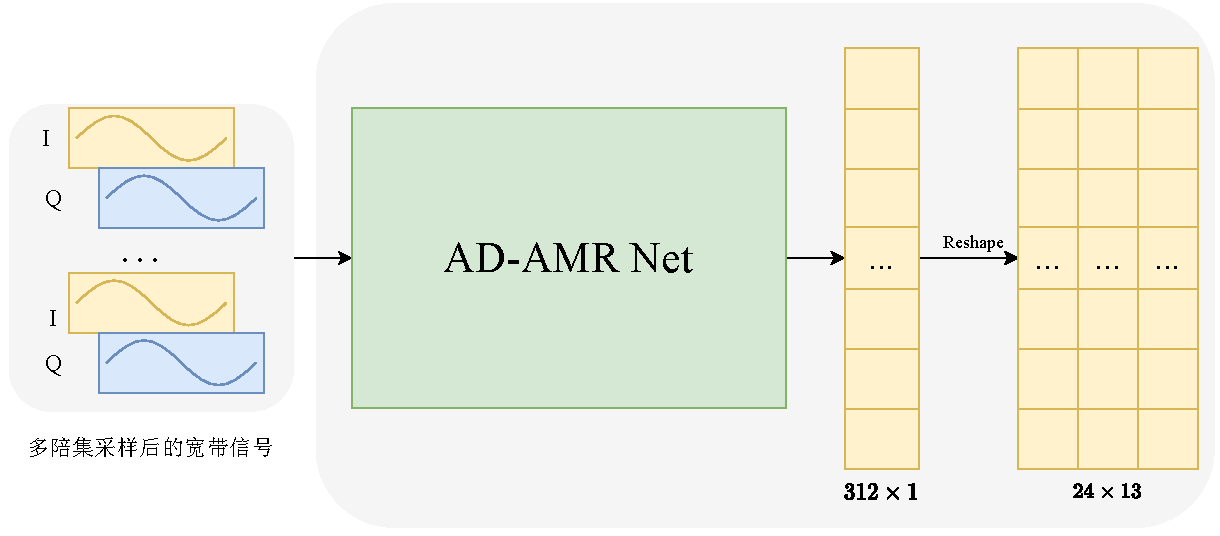
\includegraphics[width=\textwidth]{Image/plana.pdf}
    \caption{方案一:利用AD-AMR Net进行多用户场景下的宽带信号调制识别}
    \label{fig:plana}
\end{figure}

在多用户场景下的宽带信号调制识别的实验方案一中(如图\ref{fig:plana}所示),我们采用AD-AMR Net来处理分为24个子带的宽带信号,其中每个子带可能采取13种不同的调制模式或处于空闲状态。由此,模型面临的挑战是在这些子带中正确预测各种状态,总计达到\(24 \times 13\)种可能的情况。

实验的设计考虑到了信号的复杂性,尤其是在多用户环境下,信号的处理不仅需要准确识别调制模式,还需区分各个子带的特定状态。图\ref{fig:plana}展示了从接收的IQ信号开始,如何通过AD-AMR Net进行处理,并最终对每个子带的调制状态进行预测的简化流程。特别地,图中强调了信号预处理、网络处理以及重塑输出以适应大规模多分类任务的过程。

本次实验的主旨在于为整个研究建立一个性能基准线。在此方案中,网络性能的最优化并非首要目标,而是作为未来策略改进和比较的基础。此基线模型不仅提供了初始的性能指标,而且为后续采用更高级策略(例如分步骤识别或多任务学习方法)的效能评估提供了重要的比较基础。通过这种方法,我们可以清晰地定义后续方案需超越的性能门槛,并为评估AD-AMR Net在处理更复杂多用户场景时的潜力提供了一个参考点。


\subsubsection{方案二:分步骤识别}\label{sec:background}

\begin{figure}
    \centering
    \includegraphics[width=\textwidth]{Image/localization.pdf}
    \caption{方案二中的定位网络架构,用于识别活跃子带}
    \label{fig:planb_localization}
\end{figure}

在这种策略中,问题被分解为两个主要步骤:子带活跃性检测(支撑集获取)和调制模式识别,每个步骤都由专门设计的网络处理。

如图\ref{fig:planb_localization}所示,定位网络首先接收信号作为输入,并通过一系列残差块和卷积层来处理信号。这个网络的设计重点在于利用残差连接和深层卷积网络的强大特征提取能力,以准确地定位哪些子带是活跃的。通过归一化和全连接层的处理,网络最终输出每个子带活跃与否的概率分数,这些分数随后被用于识别活跃的子带。

一旦活跃子带被成功识别,如图\ref{fig:planb_classification}所示的分类网络则负责进一步分析这些子带的调制模式。该网络采用了支撑集来处理已定位的活跃子带,并通过AD-AMR Net的高效特征提取和分类能力,实现对各种调制模式的精确识别。共享全连接层和归一化步骤确保了模型可以从子带特征中提取有用信息,并有效分类调制模式。

\begin{figure}
    \centering
    \includegraphics[width=\textwidth]{Image/classification_cn.pdf}
    \caption{方案二中的分类网络架构,用于识别活跃子带的调制模式}
    \label{fig:planb_classification}
\end{figure}

通过将调制识别问题分解为两个简化的任务,方案二不仅提高了识别的准确性,还增强了模型在多用户场景下的适应性和效率。定位网络和分类网络的结合,为解决复杂的宽带信号调制识别问题提供了一种有效且清晰的解决方案,展示了分步骤识别策略在提高性能和准确率方面的潜力。
\subsubsection{方案三:多任务学习}\label{sec:background}

\begin{figure}
    \centering
    \includegraphics[width=\textwidth]{Image/planc.pdf}
    \caption{采用多任务学习方法进行宽带信号调制识别的方案三}
    \label{fig:planc}
\end{figure}
在方案三中,我们探讨了一种多任务学习方法,旨在通过单一的模型架构同时处理多用户宽带信号中子带检测和调制类型识别的双重任务。如图\ref{fig:planc}所示,这种方法的关键在于引入一个共享的特征提取模块,该模块能够捕获信号的全局特征,随后通过两个独立的任务特定头部(一个用于子带定位,另一个用于调制识别)来分别解决子带检测和调制类型识别的问题。

方案三的核心在于其高效的学习机制,通过共享特征提取模块捕获信号的全局特性,然后利用两个独立的任务特定头部同时进行子带检测和调制类型识别。这不仅降低了模型的复杂度,而且通过两个子任务的相互协作,增强了模型对复杂信号环境的适应能力。共享的特征提取模块使得模型能够在不同任务之间共享底层特征,从而提高了学习的效率和效果。

如图\ref{fig:planc}展示的,该方法首先对输入的IQ信号进行处理,通过AD-AMR Net提取信号的特征图,然后分别通过定位头和调制识别头进行子带活跃性检测和调制模式的识别。定位头负责判断哪些子带是活跃的,而调制识别头则针对检测到的活跃子带进行调制模式的精确识别。

通过这种设计,方案三实现了一种高效且灵活的方式来处理多用户场景下宽带信号的调制识别问题。通过多任务学习,模型能够在保持高性能的同时,更加高效地解决复杂的宽带信号处理任务,展现了多任务学习方法在提升识别准确性和模型效率方面的潜力。


\subsection{实验设计与评估}\label{sec:experiment_design_evaluation}

本研究的实验设计基于GBSense 2022 Advance数据集,旨在评估不同模型在多用户宽带信号调制识别任务上的性能。数据集提供了复杂的宽带信号样本,适合于测试模型在识别多种调制类型中的效能。

\paragraph{数据集} GBSense 2022 Advance数据集包括多种调制类型的信号样本,每个样本由24个子带组成,每个子带可能采用13种不同的调制模式或处于空闲状态,构成了一个高度复杂的多分类问题。

\paragraph{评价指标} 为全面评估模型性能,我们采用以下指标:
\begin{itemize}
    \item 子带活跃性检测准确率
    \item 调制类型识别准确率
    \item 总体识别准确率
    \item 模型参数量和计算效率
\end{itemize}

由于宽带信号中子带活跃性检测的困难性,我们引入了两种准确率指标,\textit{accuracy1}和\textit{accuracy2},以更细致地评估模型在此任务上的表现。

\begin{itemize}
    \item \textbf{\textit{accuracy1}(严格准确率)}:该指标要求模型的预测结果与实际状态完全一致才视为成功。例如,若实际子带活跃状态为$[0, 1, 1, 0]$,只有模型预测结果也完全为$[0, 1, 1, 0]$时,此预测才被认定为成功(计分为1);任何其他预测结果都视为失败(计分为0)。这种方式强调了完全准确的预测,不允许存在任何误差。严格准确率将被运用于最终准确率的评估中,以全面评估模型在子带活跃性检测任务中的性能。
    
    \item \textbf{\textit{accuracy2}(宽容准确率)}:考虑到任务的难度,\textit{accuracy2}提供了一种更为宽容的评估方法。若模型能完全准确预测子带的活跃状态(如预测$[0, 1, 1, 0]$且实际也为$[0, 1, 1, 0]$),则认为是完全成功(计分为2)。若预测结果部分接近实际情况(如实际为$[0, 1, 1, 0]$,预测为$[0, 1, 0, 0]$),则认为是部分成功(计分为1)。对于预测与实际情况差距较大的情况(如实际为$[0, 1, 1, 0]$,预测为$[1, 0, 1, 0]$),则视为失败(计分为0)。此方法允许一定程度的误差,同时根据预测的准确程度进行分级打分。宽容准确率将被用于神经网络的训练过程中,以确保训练时能够融合更多的信息。
\end{itemize}


考虑到宽带信号子带活跃性检测的稀疏性特点,即活跃子带相比非活跃子带在样本中出现的频率远低,我们采用了焦点损失(Focal Loss)作为训练神经网络的损失函数,以解决类别不平衡的问题。焦点损失的表达式为:

\begin{equation}
FL(p_t) = -\alpha_t (1 - p_t)^\gamma \log(p_t),
\end{equation}

其中,$p_t$是模型对于每个类别预测的概率,$\alpha_t$是针对每个类别的权重,$\gamma$是调整易分类样本贡献的聚焦参数。通过这种方式,焦点损失使模型更加专注于难以分类的少数类别,从而提高了在存在显著类别不平衡时的识别性能。

为了综合评估模型在子带活跃性检测任务上的表现,\textit{accuracy2}被采用作为评价指标。这种宽容准确率允许我们更加细致地衡量模型对于活跃子带预测的准确性,同时考虑到完全正确和部分正确的预测。通过结合使用焦点损失和\textit{accuracy2}评价指标,我们旨在促进神经网络在处理类别不平衡且具有挑战性的宽带信号子带活跃性检测任务中的训练效率和性能。


\paragraph{实验设置} 实验在Ubuntu操作系统上基于PyTorch框架进行,利用NVIDIA RTX 3090 GPU进行加速。我们遵循标准的数据集划分比例(训练集60\%,验证集20\%,测试集20\%),并设置所有模型训练至少100个epochs,采用早停机制防止过拟合,同时也采用了平台期衰减学习率来动态调整学习率。为了优化模型性能,使用随机梯度下降(SGD)优化器和交叉熵损失函数进行训练。

\paragraph{实验方案简述} 本研究设计了三种实验方案:基线模型(方案一)、分步骤识别(方案二)、和多任务学习(方案三)。这些方案被设计来探索不同策略对提高多用户宽带信号调制识别效率和准确率的影响。通过比较这些不同方案的性能,我们期望得出哪些策略在实际应用中最为有效,从而为后续的研究和实际部署提供指导。

通过这套综合的实验设计和评估标准,我们旨在深入理解不同策略在解决复杂的调制识别任务中的潜力和限制,为未来宽带信号处理的研究提供实验基础和理论支撑。



\subsection{结果分析}\label{sec:background}

\begin{table}[ht]
    \centering
    \caption{不同模型的性能比较}
    \label{tab:model_performance}
    \resizebox{\textwidth}{!}{
    \begin{tabular}{lcccc}
    \hline
    \textbf{方案} & \textbf{模型参数量} & \textbf{收敛Epoch数} & \textbf{子带活跃状态Accuracy1} & \textbf{调制识别Accuracy1} \\ \hline
    方案一 & 8.9M & 74 & 99.9\% & 23.8\% \\
    方案二 & 2.7M & 31 + 56 & 99.9\% & 87.1\% \\
    方案三 & 1.6M & 64 & 99.9\% & 94.3\% \\
    \hline
    \end{tabular}
    }
\end{table}

根据表\ref{tab:model_performance}中的结果,我们可以进行以下分析:

方案一,作为基线模型,拥有8.9M的模型参数量和需要74个Epochs才能收敛。尽管在子带活跃状态检测上达到了极高的准确率(99.9\%),表明模型能够非常准确地判断子带是否活跃,但在调制识别任务上的表现相对较弱,仅有23.8\%的准确率。这表明单一策略在处理复杂的调制识别任务时可能面临挑战,尤其是在没有专门针对调制识别优化的情况下。

方案二采用了分步骤的识别方法,显著减少了模型参数量至2.7M,并以两阶段的训练过程(分别为31个和56个Epochs)达到收敛。这种方法同样在子带活跃状态检测上取得了99.9\%的高准确率,同时在调制识别任务上的表现大幅提升至87.1\%。这一改进证明了通过将问题分解为两个相对简单的任务,模型能够更专注于各自的挑战,从而提高特定任务的识别准确率。

方案三通过实施多任务学习策略,进一步降低了模型的参数量至1.6M,且在64个Epochs内达到收敛。该方案在子带活跃状态检测上同样实现了99.9\%的准确率,并且在调制识别任务上达到了94.3\%的高准确率,表现最佳。这一结果突显了多任务学习在提高模型对复杂信号处理能力的同时,还能维持高效的模型规模和较快的训练速度。

综上所述,虽然所有方案在子带活跃状态检测上均表现出色,但在调制识别准确率上,采用分步骤识别(方案二)和多任务学习(方案三)的策略明显优于单一策略(方案一)。尤其是方案三,不仅在调制识别任务上达到了最高准确率,而且具有最低的模型参数量和相对较快的收敛速度,展现了在处理多用户宽带信号调制识别问题时的显著优势。这些发现为未来在类似任务上的模型选择和策略优化提供了重要的参考和指导。

\section{宽带信号调制解调}\label{sec:mod_demod}

随着多任务学习策略在宽带信号调制识别任务中取得显著进展,我们进一步探索了该策略在调制信号解调方面的应用。本节将详细介绍该策略在处理单用户和多用户宽带信号调制解调任务中的应用和潜力。

\subsection{单用户宽带信号调制解调}


\begin{figure}
    \centering
    \includegraphics[width=\textwidth]{Image/adamr-wideband_demodulate.pdf}
    \caption{单用户场景下的调制解调流程图}\label{fig:demode_single}
\end{figure}

对于单用户场景,本研究采用GBSense 2023 Basic数据集进行实验。该数据集提供了丰富的单用户宽带信号样本,涵盖了多种调制模式,为深入研究调制解调技术提供了理想的测试平台。通过利用多任务学习策略,这部分实验不仅旨在准确识别信号的调制类型,还致力于从调制信号中准确恢复出原始信息,以评估和验证该策略在解调过程中的有效性和效率。该实验的主要思路如\ref{fig:demode_single}所示,具体来说,通过多任务的神经网络先使用一个共享的网络来提取信号特征,然后用不同的头(卷积层)来提取信号的其他信息(调制模式、符号长度等)。结合这些信息能够得到比特流的长度,最后结合主干网络所学习到的特征以及比特流的长度信息,最终可以获取所解调信号的比特流。

\subsection{多用户宽带信号调制解调}
\begin{figure}
    \centering
    \includegraphics[width=0.8\textwidth]{Image/adamr-wideband_demodulate_mul.pdf}
    \caption{多用户场景下的调制解调流程图}\label{fig:demode_multiple}
\end{figure}

针对多用户场景,我们使用GBSense 2023 Advance数据集作为研究基础。相较于单用户场景,多用户宽带信号的调制解调任务在复杂度上有所增加,因为需要同时处理来自多个用户的信号,并准确地区分和解调各自的调制信号。多任务学习策略在此场景下的应用,旨在通过共享的特征提取模块捕获信号的全局特性,并利用任务特定的子模型分别进行子带检测和调制类型识别,从而实现高效准确的调制解调性能。如图\ref{fig:demode_multiple}所示,该策略的核心在于采取了“分而治之”的策略,先通过一个频谱感知网络获取信号的全局特征和支撑集信息,然后将信号分别送入两个独立的解调网络进行解调,在这里的解调网络和之前的单用户场景下的网络结构整体上是一直的,在训练时,各个子解调模块只专注于属于自己子带编号上的信号解调,这样能够有效提高解调的准确性。

\subsection{实验设计与结果}

\subsubsection{单用户宽带信号调制解调实验}

本节详述了单用户宽带信号调制解调任务的实验设计及其结果。实验使用GBSense 2023 Basic数据集,并采用多任务学习方法,其中AD-AMR Net负责特征提取,并结合了多个专用头部进行不同任务的识别与解调。
由于是多任务模型,该实验的评价指标将结合各个子任务的性能来探究。
\begin{itemize}
    \item \textbf{误码率 (Bit Error Rate, BER)}:评估解调后的比特流中错误比特的比率。
    \item \textbf{信号长度识别准确率 (Length Accuracy)}:评估模型预测信号长度的准确性。
    \item \textbf{调制类型识别准确率 (Modulation Accuracy)}:评估模型识别调制模式的准确性。
    \item \textbf{符号长度识别准确率 (Symbol Length Accuracy)}:评估在符号级别上模型预测信号长度的准确性。
\end{itemize}

经过训练和测试,模型在单用户宽带信号调制解调任务上取得如下结果:
\begin{itemize}
    \item 比特错误率为 \(0.08423166826246754\)
    \item 信号长度识别准确率为 \(0.9613283125\)
    \item 调制类型识别准确率为 \(0.9762173502441833\)
    \item 符号级长度识别准确率为 \(0.98077253547484202\)
\end{itemize}

实验结果表明,AD-AMR Net在单用户宽带信号的调制解调任务上表现优秀,特别是在调制类型和符号级长度的识别上。这一结果为单用户宽带信号解调提供了一种有效的解决方案,同时验证了多任务学习策略在解决此类复杂信号处理问题中的潜力和实用性。

\subsubsection{多用户宽带信号调制解调实验}
\dots
目前BER还是很高,需要进一步优化模型。
\dots

\section{本章总结}\label{sec:background}
在本章中,我们深入探讨了宽带信号多用户调制识别的问题。面对复杂的多用户通信环境,我们提出并测试了三种不同的策略来解决宽带信号的调制识别问题。

首先,我们实现了一个基线模型,该模型直接预测所有可能的子带位置和调制类型组合。这种方法为我们提供了一个初步的性能基准,虽然简单但在某些情况下能够有效工作。随后,我们探索了一种分步骤的方法,先识别子带位置,再进行调制识别。这种策略使我们能够更精细地处理信号,提高了识别的准确性。

最后,我们采用了一种多任务学习策略,该策略在总体上对亚采样信号进行特征提取,然后通过不同的头实现子带位置的判别和调制模式的识别。这种方法通过共用特征提取模块减少了模型的复杂度,并增加了两个子任务的关联性,从而在保持高效率的同时提高了识别的准确度。

受到宽带调制识别中多任务方法的启发,我们进一步拟出并实现了对亚采样宽带信号直接解调的框架,在单用户场景下取得了一定的成果。这一新策略不仅补充了之前方法的局限性,还拓宽了我们对宽带信号处理能力的认识。

通过对这些方法的实验评估,我们不仅验证了它们在多用户宽带信号调制识别任务中的有效性,还展示了各种策略的优势和局限性。这些实验结果为未来在宽带信号处理和调制识别领域的研究提供了有价值的见解,特别是在设计适应复杂通信环境的算法时。我们相信,本章的研究工作将对未来的技术发展和应用实践产生积极影响,为处理更为复杂的通信系统中的挑战提供了可行的解决方案和方法。

\chapter{总结与展望}\label{chap:intro}
\markboth{第五章\ \ 总结与展望}{}
\section{研究工作总结}\label{sec:background}

在当今的数字时代,无线通信技术的发展至关重要。随着通信技术的进步,调制识别成为了无线信号处理领域的一个关键问题,特别是在军事和民用通信系统中。调制识别不仅能够提高通信系统的效率和安全性,还能够在无线频谱管理和干扰检测中发挥重要作用。深度学习方法的出现为调制识别提供了新的解决方案,然而,现有的深度学习模型在处理噪声干扰和多用户干扰时仍然存在一定的局限性。因此,如何提高调制识别的性能,特别是在宽带信号处理和多用户场景下,成为了当前研究的重点问题。

围绕以上问题,本文主要做了以下工作和创新点。

1.介绍了调制识别的研究背景及其在国内外的研究现状。对传统调制识别方法和深度学习方法进行了详细的介绍和分析,为后续章节的研究提供了理论基础和技术支持。

2.对理论基础进行了深入的探讨,包括数字调制的基本原理与特性、深度学习的基本原理和技术特点,压缩感知理论等。这些理论基础为后续章节的研究提供了坚实的理论基础。

3.提出的自适应噪声矫正调制识别网络(AD-AMR)模型,旨在解决调制识别过程中的噪声干扰问题。通过在RadioML 2016和RadioML 2018数据集上的实验验证,AD-AMR展示了优于现有方法的性能。详细介绍了AD-AMR模型的架构设计、关键组件以及实验设置,包括模型在不同噪声条件下的性能比较,以及与其他深度学习模型的比较分析。这些实验结果不仅验证了AD-AMR模型的有效性,也展示了深度学习技术在调制识别领域的应用潜力。

4.进一步扩展了AD-AMR模型的应用范围,将研究重点转向了更为复杂的宽带信号处理,特别是在单用户和多用户场景下的性能评估。通过对单用户场景的初步实验,验证了AD-AMR模型在处理宽带信号调制识别任务中的有效性。针对多用户场景,提出了多种方案,并通过实验比较得出多任务学习方法在处理复杂场景中的前景。此外,还探讨了将任务衍生到宽带信号调制解调的可能性,并在单用户场景解调上取得了一定的效果。最后,提出了在多用户场景解调时可以沿用的架构,为未来在宽带信号处理领域的研究提供了新的思路和方法。


\section{未来工作展望}\label{sec:background}

在对未来工作的展望部分,本研究虽然在调制识别领域取得了一定的进展,但仍存在一些不足之处,这些不足为未来的研究方向提供了明确的指向。首先,本文在模型轻量化方面的工作还未达到极致,尤其是在模型剪枝方面。模型轻量化是实现高效计算和降低模型部署成本的关键,对于在资源受限的设备上实现实时调制识别尤为重要。因此,未来的工作可以探索更高效的模型压缩和剪枝技术,以进一步减少模型的计算需求和存储需求,同时保持或提升模型的性能。

其次,本研究没有对多种压缩率场景下的采样信号进行详尽的结果分析。在实际应用中,不同的压缩率对调制识别的性能有显著影响,尤其是在宽带信号处理中。未来的工作应该重点关注不同压缩率下的采样策略和调制识别性能,通过深入分析不同压缩率对识别准确率的影响,优化采样过程,以适应更广泛的应用场景和需求。

此外,尽管本研究在单用户调制识别方面取得了一定的成果,但在多用户调制解调上的效果并不理想。这表明在处理多用户场景下的复杂信号时,可能还需要从信号的压缩采样角度进行深入的量化分析和研究。多用户场景下的调制解调问题涉及到信号的分离、干扰消除等多个方面,因此未来的研究可以探索结合信号处理和深度学习的新方法,如信号压缩采样和高级解调技术,以提高在多用户环境下的调制识别和解调性能。

最后,未来的工作还应该考虑实现模型的自适应和动态调整能力,以更好地适应变化多端的通信环境和信号条件。这包括开发能够根据当前环境条件自动调整其参数和结构的智能模型,以及利用在线学习和增量学习策略来持续优化模型性能。通过这些努力,未来的调制识别系统将能够更加灵活和高效地应对各种挑战,为无线通信领域的发展贡献力量。
%- 
\backmatter% 初始化其他部分环境,不建议注释
%-
\szubibliography% 导入参考文献
%-
\chapter[附录]{附录A\ \ xxxxxx}
\markboth{附录A\ \ xxxxxx}{}

% 导入附录
\chapter*{附录B\ \ xxxxxx}
\markboth{附录B\ \ xxxxxx}{}

%-
%- 2020年新增,添加答辩记录,建议分成三个独立的PDF文件,
%- \szuaddpdf命令包含两个参数,[]中为可选参数,用于生成目录,{}中为PDF文件名,默认在Image下
% \szuaddpdf[指导教师对研究生学位论文的学术评语]{pingyu}
% \szuaddpdf[学位论文答辩委员会决议书]{dabian1}
%-\szuaddpdf{dabian2}% 前一页生成目录即可
%-
\chapter[致谢]{致\quad{}谢}
\markboth{致谢}{}

在完成这项研究工作的过程中,我深深体会到了团队合作与各方支持的重要性。因此,在此,我衷心感谢所有直接或间接帮助、指导和支持我的人们。

首先,我要特别感谢我的导师,她不仅在专业知识上给予我深刻的指导,还在研究方法和学术态度上对我产生了深远的影响。她严谨的学术态度、勤奋的工作精神和无私的指导精神,让我受益匪浅。在研究过程中遇到的每一个难题,导师都耐心地指导我思考和解决,她的智慧和经验对我完成这项工作至关重要。

同时,我也要感谢我的研究小组成员。在整个研究过程中,我们共同探讨、互相帮助,共同克服了一个又一个难关。每个成员的勤奋和智慧都为这项研究的成功奠定了基础。我们之间的讨论常常激发出新的思想火花,这些宝贵的思想交流对我的研究有着不可或缺的贡献。

此外,我还要感谢参与本研究的所有同行和学者。在进行文献综述和研究设计时,他们的研究成果为我提供了宝贵的参考和灵感。同时,我也感激那些在学术会议和研讨会上给予我建议和反馈的专家们,他们的批评和指导使我的研究工作更加完善。

感谢我的家人对我学术道路上无条件的支持和鼓励。在我遇到困难和挫折时,是他们给了我力量和勇气,让我能够坚持下去。他们的理解和爱是我最坚强的后盾。

我还要感谢我的朋友们,他们的陪伴和支持使我的研究生活充满欢笑和温暖。在繁忙和压力之余,与他们的交流和放松对我保持良好的精神状态至关重要。

最后,感谢所有阅读这篇论文的人。希望我的工作能够对您有所帮助,也期待未来能够与更多的同行和读者分享和讨论研究成果。

在此,我再次向所有支持和帮助我的人表示最诚挚的感谢。是你们的帮助和支持,让我能够顺利完成这项研究工作。未来的道路上,我将继续努力,不忘初心,砥砺前行。% 导入致谢
%-
\chapter{攻读硕士学位期间的研究成果}
\markboth{攻读硕士学位期间的研究成果}{}
%- 可以直接使用引用的格式

\begin{enumerate}[label = {[\arabic*]}]
    \item 基于开源平台的持续集成功能测试系统. 2022
    \item Adaptive Denoising With Efficient Channel Attention for Automatic Modulation Recognition. 2024
\end{enumerate}


%- 或者区分开

% \section*{论文}

% \begin{enumerate}[label = {[\arabic*]}]
%     \item TANG T T. xxx xxxx xx xxx. IEEE Transactions on xxxx. 2020.
% \end{enumerate}

% \section*{专利}

% \begin{enumerate}[label = {[\arabic*]}]
%     \item 唐同学. 一种基于某某的方法:中国,01100000.5. 2020-01-01.
% \end{enumerate}% 导入研究成果
%-
\end{document}
% %---------------------------------------------------------------------------%
